%%%%%%%%%%%%%%%%%%%%%%%%%%%%%%%%%%%%%%%%%
% Masters/Doctoral Thesis 
% LaTeX Template
% Version 1.41 (9/9/13)
%
% This template has been downloaded from:
% http://www.latextemplates.com
%
% Original authors:
% Steven Gunn 
% http://users.ecs.soton.ac.uk/srg/softwaretools/document/templates/
% and
% Sunil Patel
% http://www.sunilpatel.co.uk/thesis-template/
%
% License:\emph{•}
% CC BY-NC-SA 3.0 (http://creativecommons.org/licenses/by-nc-sa/3.0/)
%
% Note:
% Make sure to edit document variables in the Thesis.cls file
%
%%%%%%%%%%%%%%%%%%%%%%%%%%%%%%%%%%%%%%%%%

%----------------------------------------------------------------------------------------
%	PACKAGES AND OTHER DOCUMENT CONFIGURATIONS
%----------------------------------------------------------------------------------------

\documentclass[twoside, openright, titlepage]{Thesis} % Paper size, default font size and one-sided paper

\graphicspath{{Pictures/}{../Pictures/}} % Specifies the directory where pictures are stored

\usepackage{natbib}
\bibliographystyle{agsm}

\hypersetup{urlcolor=blue, colorlinks=true} % Colors hyperlinks in blue - change to black if annoying

\title{\ttitle} % Defines the thesis title - don't touch this

%\usepackage{pgfplots}
%\pgfplotsset{compat=1.4}
%\usepackage{tikz}

\newcommand\nop[1]{}
\newcommand\note[1]{{\color{red}[#1]}}
\newcommand\rewrite{\note{Rewrite in different way}}


\usepackage{setspace} % just to enable Conor to print in double space
\usepackage[linesnumbered,ruled,vlined]{algorithm2e}
\usepackage{enumitem}
\usepackage{float}

\usepackage{listings}
\usepackage{multirow}
% ===================Tikzpicture=============================================================
%\usepackage{tikz}
%\usepackage{graphicx}
%\usetikzlibrary{patterns}
%\usetikzlibrary{arrows, decorations.markings}
%==========================================================
\usepackage{todonotes}


%=====language============================================
\usepackage{xcolor}
\usepackage{bold-extra}

\definecolor{background}{HTML}{EEEEEE}

% Language Definitions for SPARQL
%\lstdefinelanguage{sparql}{
%	basicstyle=\normalsize\ttfamily,
%	breaklines=true,
%	frame=single,
%   backgroundcolor=\color{background},
%	morecomment=[l][\color{olivegreen}]{\#},
%	morestring=[b][\color{blue}]\",
%	morekeywords={SELECT,CONSTRUCT,DESCRIBE,ASK,WHERE,FROM,NAMED,PREFIX,BASE,OPTIONAL,FILTER,GRAPH,LIMIT,OFFSET,SERVICE,UNION,EXISTS,NOT,BINDINGS,MINUS,a},
%	sensitive=true
%}

\lstdefinelanguage{sparql}
{
	frame=single,
	basicstyle=\normalsize\ttfamily,
	backgroundcolor=\color{background},
    breaklines=true,
	morestring=[b][\color{blue}]\",
	morekeywords={SELECT,CONSTRUCT,DESCRIBE,ASK,WHERE,FROM,NAMED,PREFIX,BASE,OPTIONAL,FILTER,GRAPH,LIMIT,OFFSET,SERVICE,UNION,EXISTS,NOT,BINDINGS,MINUS,a,ORDER,BY,GROUP},
	sensitive=true
}

\lstdefinelanguage{snapshot}
{
	frame=single,
	basicstyle=\scriptsize\ttfamily,
	backgroundcolor=\color{background},
    breaklines=true,
}

%=========================================================
\begin{document}

%\listoftodos

\frontmatter % Use roman page numbering style (i, ii, iii, iv...) for the pre-content pages

% Define the page headers using the FancyHdr package and set up for one-sided printing
\fancyhead{} % Clears all page headers and footers
\rhead{\thepage} % Sets the right side header to show the page number
\lhead{} % Clears the left side page header

\pagestyle{fancy} % Finally, use the "fancy" page style to implement the FancyHdr headers

\newcommand{\HRule}{\rule{\linewidth}{0.5mm}} % New command to make the lines in the title page

% PDF meta-data
%\hypersetup{pdftitle={\ttitle}}
%\hypersetup{pdfsubject=\subjectname}
%\hypersetup{pdfauthor=\authornames}
%\hypersetup{pdfkeywords=\keywordnames}

%----------------------------------------------------------------------------------------
%	TITLE PAGE
%----------------------------------------------------------------------------------------

\begin{titlepage}
\begin{center}


\includegraphics{nuig-new.pdf} % University/department logo - uncomment to place it

\textsc{}\\[1cm] 

{\huge \bfseries Processing Linked Data on\\Lightweight Computing Devices}\\[3cm] % Thesis title

{\LARGE \textbf{Anh, Le-Tuan}}\\[2cm]

\large {Submitted in fulfilment of the requirements\\ for the degree of Doctor of Philosophy}\\[2cm] 

{\LARGE \textsc{SUPERVISORS:}\\ \textbf{Dr. Conor Hayes}\\ \textbf{Dr. Danh Le Phuoc}\\[3.5cm] }

\HRule \\[0.0cm]

\large {Insight Centre for Data Analysis, National University of Ireland, Galway}\\
{\large September 2018}  % Date

\vfill
\end{center}
\end{titlepage}


%----------------------------------------------------------------------------------------
% BLANK PAGE
%----------------------------------------------------------------------------------------
%\textsc{}
%\clearpage % Start a new page
%---------------------------------------------------------------------------------------


%----------------------------------------------------------------------------------------
%	QUOTATION PAGE
%----------------------------------------------------------------------------------------

%\pagestyle{empty} % No headers or footers for the following pages
%\null\vfill % Add some space to move the quote down the page a bit
%\begin{flushright}
%\LARGE \textit{``If you optimize everything you will always be unhappy."}\\
%Donald Knuth
%\end{flushright}
%\vfill\vfill\vfill\vfill\null % Add some space at the bottom to position the quote just right
%\clearpage % Start a new page


%----------------------------------------------------------------------------------------
% BLANK PAGE
%----------------------------------------------------------------------------------------
%\textsc{}
%\clearpage % Start a new page
%---------------------------------------------------------------------------------------
%----------------------------------------------------------------------------------------
%	ABSTRACT PAGE
%----------------------------------------------------------------------------------------

%\addtotoc{Abstract} % Add the "Abstract" page entry to the Contents
%
%\abstract{\addtocontents{toc}{}
%
%
% 
%} % Add a gap in the Contents, for aesthetics
%
%\clearpage % Start a new page

%----------------------------------------------------------------------------------------
%	ACKNOWLEDGEMENTS
%----------------------------------------------------------------------------------------

%\setstretch{1.1} % Reset the line-spacing to 1.3 for body text (if it has changed)

%\acknowledgements{\addtocontents{toc}{} % Add a gap in the Contents, for %aesthetics
%
%
%}
%\clearpage % Start a new page

%----------------------------------------------------------------------------------------
%	LIST OF CONTENTS/FIGURES/TABLES PAGES
%----------------------------------------------------------------------------------------

\pagestyle{fancy} % The page style headers have been "empty" all this time, now use the "fancy" headers as defined before to bring them back

\lhead{\emph{Contents}} % Set the left side page header to "Contents"
\tableofcontents % Write out the Table of Contents

%\lhead{\emph{List of Figures}} % Set the left side page header to "List of Figures"
%\listoffigures % Write out the List of Figures

%\lhead{\emph{List of Tables}} % Set the left side page header to "List of Tables"
%\listoftables % Write out the List of Tables

%----------------------------------------------------------------------------------------
%	ABBREVIATIONS
%----------------------------------------------------------------------------------------
%\clearpage % Start a new page
%\setstretch{1.5} % Set the line spacing to 1.5, this makes the following tables easier to read
%\lhead{\emph{Abbreviations}} % Set the left side page header to "Abbreviations"
%\listofsymbols{ll} % Include a list of Abbreviations (a table of two columns)
%{
%\textbf{LAH} & \textbf{L}ist \textbf{A}bbreviations \textbf{H}ere \\
%%\textbf{Acronym} & \textbf{W}hat (it) \textbf{S}tands \textbf{F}or \\
%}
%
%----------------------------------------------------------------------------------------
%	PHYSICAL CONSTANTS/OTHER DEFINITIONS
%----------------------------------------------------------------------------------------
%
%\clearpage % Start a new page
%
%\lhead{\emph{Physical Constants}} % Set the left side page header to "Physical Constants"
%
%\listofconstants{lrcl} % Include a list of Physical Constants (a four column table)
%{
%Speed of Light & $c$ & $=$ & $2.997\ 924\ 58\times10^{8}\ \mbox{ms}^{-\mbox{s}}$ (exact)\\
% Constant Name & Symbol & = & Constant Value (with units) \\
%}
%
%----------------------------------------------------------------------------------------
%	SYMBOLS
%----------------------------------------------------------------------------------------
%
%\clearpage % Start a new page
%
%\lhead{\emph{Symbols}} % Set the left side page header to "Symbols"
%
%\listofnomenclature{lll} % Include a list of Symbols (a three column table)
%{
%$a$ & distance & m \\
%$P$ & power & W (Js$^{-1}$) \\
%% Symbol & Name & Unit \\
%
%& & \\ % Gap to separate the Roman symbols from the Greek
%
%$\omega$ & angular frequency & rads$^{-1}$ \\
%% Symbol & Name & Unit \\
%}
%
%----------------------------------------------------------------------------------------
%	DEDICATION
%----------------------------------------------------------------------------------------
%
%\setstretch{1.3} % Return the line spacing back to 1.3
%
%\pagestyle{empty} % Page style needs to be empty for this page
%
%\dedicatory{For/Dedicated to/To my\ldots} % Dedication text
%
%\addtocontents{toc}{\vspace{2em}} % Add a gap in the Contents, for aesthetics
%
%----------------------------------------------------------------------------------------
%	THESIS CONTENT - CHAPTERS
%----------------------------------------------------------------------------------------

\mainmatter % Begin numeric (1,2,3...) page numbering
\setstretch{1.1}
\setlength{\parskip}{8pt plus10pt minus10pt}

\pagestyle{fancy} % Return the page headers back to the "fancy" style

% Include the chapters of the thesis as separate files from the Chapters folder
% Uncomment the lines as you write the chapters

%\chapter{Introduction}
\label{ch:introduction}
\lhead{Chapter 1. Introduction(by August)}
%---------------------------------------------------------------------------------%
\section{Motivation}

Pervasive computing and the Internet of Things(IoT) are about making our lives simpler by providing smart environments with intelligent applications, services as ubiquitous assistants~\citep{Weiser:99}. 
The smart applications, services are built based on digital environments that are created by massive of interconnecting smart devices.
Despite of the different focus~\citep{Ebling:2017}, on human-centric or globally, both of the visions (of IoT and pervasive computing) are recognised on the evolution of digital technologies that are related to sensing, computing and communicating technologies. 
The smart applications, services are created with the same principle that collect real-world data from sensors, create situation context and make the respond adaptively to the context.

As the real-world data is collected from a number of different devices, this is usually multi-model and diverse in nature.
The pervasive computing and IoT often face with the lack of standardisation that related to data models and data format that is to represent, integrate and interpret such data~\citep{Miorandi:2012}. 
Furthermore, as in the scenario, a number of highly systems, services will need to communicate autonomously.
Providing such interoperability among the systems, services in the key enabler the smart space. 
Therefore, one of the most fundamental challenges for pervasive system and the IoT is how to model and reason the massive of data and how to enhance the sharing and interoperability across heterogeneous devices, systems and service.

A suitable solution lies in semantic technologies, particularly the Semantic Web which aims to support capturing intended semantics and automated reasoning, therefore, enabling sharing and integrating information from heterogeneous sources~\citep{Barnaghi:2012}. 
RDF is a well established data model to describe the semantics of real data.
As well as allowing a flexible way of integrating heterogeneous data, and RDF ontology-based context description enables better reasoning and a better sharing contextual information.
There have been efforts  by the W3C Semantic Sensor Network~\footnote{https://www.w3.org/2005/Incubator/} and Web of Things group~\footnote{https://www.w3.org/WoT/} to lift sensory data to a semantic level using Semantic Web technologies. 
The goal is to make sensory data available according to the Linked Data principles~\citep{Bizer:2011} that facilitates the semantic interoperability crossing smart devices, smart platforms and smart spaces~\citep{IERC:2013}. 

RDF engines combine with cloud computing could provide scalable Linked Data management~\citep{Hauswirth:2017}.
Cloud infrastructures have been considered as an unlimited capabilities storage and processing power, and the stability of cloud computing has been close the mature stage.
Leveraging the capacity of storage and computation of the cloud, the common approaches in the IoT are to connect IoT devices to cloud where IoT data can be stored and processed.
However, cloud computing solution alone could not completely handle the scalability issue of the IoT~\citep{Zhang:2015}.
The end devices in the IoT are not only data consumers as in cloud computing paradigm but data producers.
The increase of the number of the IoT devices means the quantity of produced IoT data is raising quickly.
Most of the data can be discarded immediately after being processed.
Hence, in these centralised systems, the bandwidth would be overwhelming and might be wasted.
Furthermore, pushing data into cloud will dominate upstream network traffic, meanwhile, broadband networks have more downstream bandwidth than upstream bandwidth.
Moreover, some IoT applications might require very quick response time, unfortunately, cloud-based solution may lead these applications to be less operable due to unexpected network latencies.
In additional, IoT data might contain sensitive information from the sensors that are implanted surrounding us.
Cloud-based systems create more privacy and security concerns as centralised storages are out of users' control.

Edge computing~\citep{Salman:2015} has been the recently decentralised computing paradigm to address these issues.
\cite{WShi:2016} explained that ``edge computing refers to the enabling technologies allowing computation to be performed at the edge of the network,
on downstream data on behalf of cloud services and upstream data on behalf of IoT services".
\cite{WShi:2016} also defined the ``edge" as ``any computing and network resources along the path between data sources and cloud data centres".
Thus, the edge can be the smartphones as they are placed between sensors and cloud or the edge can be the gateway devices that connect smart devices and data centres.


Thanks to the recent rapid development in designing embedded devices, e.g., ARM boards, IoT gateways are getting cheaper and smaller whilst more powerful.
For example, a Raspberry PI Zero or a C.H.I.P computer costs less than 15 euro and have the size smaller than a credit card but it is powerful enough to run a fully functioning Linux distro.
Not only having advantages in power consumption and size but also being cost-effective, the devices of this kind can be easily embedded or bundled with other IoT devices (e.g., sensors and actuators) as a processing gateway interfacing with outer networks, called \emph{edge devices}. 
An exemplary deployment setting which can greatly benefit from these advantages is deploying a semantic integration gateway for an outdoor ad-hoc sensor network, e.g on a street or a traffic junction. 
This gateway can be easily fitted in the lamp pole to share the power source with a street lamp powered by a small solar panel.
In the light of embracing the pervasiveness of semantic integration gateways, we are motivated to investigate and to improve the scalability and robustness of RDF engines on this class of \emph{light weight edge devices}.

Despite, their advantages in terms of power consumption, size and cost-effectiveness, lightweight edge devices are significantly underspecified in terms of the memory and CPU demands of the available RDF engines.
Executing the data processing tasks locally on embedded devices might require much more efforts in optimising the computations or in handling limited resources. 
However, devices can be self-contained and be able to operate in different environments. 
Furthermore, data transmission costs can be dramatically reduced as it does not require the transfer of data from a device to a server. 
Working independently from a remote server also avoids the requirement for devices to maintain a frequent connection. Thus, the risks caused by intermittent connectivity can be reduced.
As device data is not stored and processed on a remote server, the privacy and security concern is also reduced. Finally, by distributing that computation among a large number of existing small but powerful devices, a greater computational scale can be achieved.

\section{Problem Statement}

The motivation leads to several research problems that arise when enable RDF data to be processed on the lightweight edge devices.
The first challenging problem is creating a tailored RDF storage for this class of devices.
Several RDF store such Jena TDB, Sesame, Virtuoso are able to operate on these devices as the computational resource on the devices is sufficient enough.
However, they are designed and optimised for personal computers (PCs) and thus are unsuitable for directly porting to edge devices. 
Due to the differences in computing environment between edge devices and PCs, the performance and storage ability of existing RDF engine that are implemented based-on PC design are limited. 

Lightweight edge devices are distinctive from PC-based workstations in two major ways: (i) they have a significantly smaller amount of main memory and (ii) they are equipped
with lightweight flash-based storage as a secondary memory.
Besides integration and processing of data, network edge devices are required to execute frequent update operations. 
For example, due to adding new devices into the network or to updating new data from connected sensors. 
To manage large static RDF datasets, existing RDF engines build sophisticated indexing mechanisms that consume a large amount of main memory and are expensive to update.
Directly applying the same approach on a memory-constrained device causes system paging behaviours or out-of-memory errors that heavily penalise performance.

Furthermore, the I/O behaviours of flash-based storage, specifically the erase-before-write limitation, degrade the efficiency of disk-based data indexing structures and caching
mechanisms.
For instance, flash-based storages store in formation in arrays of electric memory cells.
Cells are organised into pages and pages are grouped into blocks. 
A page is the smallest unit that can be read from or written to flash memory.
A block is the smallest structure that can be erased from such storage. 
On flash memory, updating a single page in the block is not possible; instead one has to erase the whole block and only then newly updated data can be written to this block.
Thus, write-in-place operation, that updates a single piece of data in a block, consists of two operations on the entire block: erase and write. 
Due to the flash I/O behaviours, the commonly used indexing structure in RDF triple store, B$^+$ Tree, is not optimal for flash-based storage.

[Therefore, ...]

The second challenge is associated with the unreliable memory issue of these edge devices. 
The lightweight devices as edge nodes might run several services.
In many scenarios, RDF engines are used as embedded semantic databases for edge applications.
The the memory for RDF engines is shared with other processes or with the hosted applications.
Therefore, in runtime, the available memory for the RDF engine may be dynamic.

Join is the most-used operation to answer SPARQL as it requires many joins of triples that match the triple patterns.
Different join algorithms requires input data is organised in different ways.
The former SPARQL query planners often select join algorithm that is suitable with the available index on the data and and query optimisers order joins to reduce the working set.
However, they did take memory consumption into account.
Using too much memory may result query failure or using insufficient memory may result the selected join algorithm become suboptimal.

[Therefore, ...]

Another challenge is how to enable the federation ...



\section{Thesis Contribution}

\subsubsection*{Flash-Awareness RDF Storage for Lightweight Edge Devices}


\subsubsection*{Memory Adaptive SPARQL Query Processing}

\subsubsection*{Federation Framework for Edge IoT}

\newpage
\section{Thesis Outline}

\textbf{Background: }
The background chapter describes the basic concepts of the IoT, the Semantic Web and basic techniques for RDF data management.
Section 2.1 provides the visions of the IoT and two emergent research topics in the IoT: describing the semantic for IoT and distributing computations among IoT nodes(edge computing).
After highlighting the promising of the Semantic Web in providing semantic annotating and processing for IoT data, the core technologies of the Semantic Web are introduced in Section 2.2. 
In this section, the RDF data model, Knowledge inference and the query language for RDF data are presented. 
For the understanding the possibility of processing RDF data on the edge devices, Section 2.3 introduces basic techniques for managing RDF data. 
The section provides an overview of how RDF data can be stored and queried from database management perspective.

\textbf{Literature Review}
In this section, we review database techniques that are relevant to IoT devices and building RDF engines. 
Section 3.1 introduce the characteristics of IoT devices.
This is critical important topic, because,  designing a database would need a brief understanding of the behaviours of the machines on which it runs.
As section 3.1 highlights the two distinctive characteristics (memory limitation and using flash-based storage) of the high-end IoT edge devices(that the thesis targets), Section 3.2 reviews the related works on database techniques that have been developed and could be used for creating RDF engine.
Section 3.3 presents several attempts to create RDF engine for small devices including sensors, smart phones.

\textbf{Empirical Study}
Several PC-based RDF engines can operate on the high-end IoT devices as computation resource of the high-end IoT edge devices is somehow sufficient enough.
This section provide a brief evaluation of PC-based RDF engines when running on these devices.
The evaluation is conducted in the IoT context. 
This section clarifies the concern of the need of the new design for RDF engines for this class of devices.

\textbf{Flash-Aware RDF Storage}

This section provide our solution to improve the performance of RDF storage for the high-end IoT devices by create flash-aware data structure for RDF data and flash-aware buffer management for managing the writes.

\textbf{Adaptive Strategy for Iterative Join Execution}

This section provide our solution for adaptive execution the joins in SPARQL.
As memory is limited on edge devices, the joins should optimised to reduce the memory consumption. 
Among the join algorithms for RDF data, nested index loop join(NILJ) consumes memory the less.
Our solution is based on NILJ and push based model to allow the adaptivity reordering the joins at runtime according to the data cached in the buffer. 

\textbf{Federation over edge nodes}

This section will provide framework allowing data federation among gateways.

\chapter{Internet of Things: Technologies and Architectures}
\label{ch:iot_tech_arch}
\lhead{Chapter 2. Internet of things: Technologies and Architectures}

The term ``\textit{Internet of Things}"(IoT) was first used in a presentation of Kevin Ashton when presenting his work in The Auto-ID Labs~\footnote{https://autoidlabs.org/}. 
Since then, this paradigm has tremendously gained attention in the scenarios of modern embedded technology, communication technology and information technology.
The IoT was, basically, to refer to an ecosystem of interconnected physical objects that are accessible through the Internet.
As technology evolved its definition has changed, and has been more inclusive covering wide range of applications~\citep{Atzori:2017}. 


Although many definitions of the IoT have been stated by different researchers, business alliances and standardisation bodies~\citep{Minerva:2015}, the main idea of the IoT is the same.
The main goal of the IoT is the integration of physical world with the virtual world that enables a ubiquitous system of sense information.
This integration is being created by enabling physical objects to perceive their surrounding environment, to connect and exchange data among each other and to communicate with people.
As a result, people will be able to monitor and interact with the physical environment remotely from the computer-based systems.
On the other hand, physical objects will be able to derive an understanding of their context, to cooperate with each other, to adaptively interact to changes of their context and thus intelligently assist people.


IoT requires the integration of several technologies.
Embedded technology enables sensors and actuators to be quipped on physical objects; thus they are able to perceive their context and react adaptively to the context.
Communication technology provides networking capabilities; hence, IoT objects can communicate with each other to exchange data an context.
Internet access and user interfaces allows interaction with or provides assistance to people from anywhere and at anytime.
Moreover, semantic, machine intelligence technologies may involve to enable context-awareness and autonomous decision making~\citep{Vermesan:2018}. 

This chapter provides the background knowledge of the Internet of Things. In particularly, section~\ref{sec:history_of_iot} introduces the development of the IoT vision. The enabling technologies for the IoT is presented in Section~\ref{sec:technologies_of_iot}. Finally, we discuss the architectures that enable the IoT in Section~\ref{sec:architecture_of_iot}

%====================================================================
\section{History of IoT}
\label{sec:history_of_iot}
\lhead{2.1 History of IoT}
%====================================================================
The IoT has been defined by researchers, business alliances and standardisation bodies from many domains and different perspectives~\citep{Minerva:2015}.
\cite{Atzori:2010} summarised that IoT would result from the convergence of three main visions: \textit{Thing-oriented vision}, \textit{Internet-oriented vision} and \textit{Semantic-oriented vision}.

%[1999]  
The very first vision of the IoT was derived from the Thing-oriented perspective.
The term ``Internet of Things" was first used in the Auto-ID lab's presentation that introduced Radio-Frequency Identification(RFID) technology. 
An RFID system is composed of RFID readers and RFID tags.
A tags has a unique identifier and is attached in a physical object.
The readers listen to the radio signal from tags to identify the appearance of physical objects in the surrounding area. 
Such RFID systems would allow physical objects to be mapped into the virtual world using RFID readers and RFID tags.
In this early stage, ``Things" simply referred to RFID tags and the IoT was a system of physical objects that were traceable via RFIDs. 
The Unique/Universal/Ubiquitous Identifier(uID)~\citep{Sakamura:2006} and the Electronic Product Code(EPC)~\citep{Armenio:2007} were the following projects that supported the worldwide use of the RFID technology.
These projects aimed to create a global standard for RFIDs that would enable the global identification for physical objects.

%[2005]
It was argued that the IoT would be built up by combing RFID technology and sensing technology~\citep{ITU:2005}.
The RFID tags could respond to the location, label and status of the tagged physical objects.
Sensors could be embedded in the physical objects to provide information about the environment surrounding the objects. 
The integration of the two technologies would enable the fuller understanding on the context of the physical objects.
Wireless sensors and RFID tags attached on moving objects would provide better status of the objects, i.e, their location and temperature, movements, etc.
The IoT vision became wider vision than the idea of a global system of RFID tagged objects, thing's intelligence was considered~\citep{Sterling:2005}. 

%[2006-2009]
According to~\cite{Presser:2009}, the IoT could be more than just a global EPC system of RFID tagged objects.
Devices, networks, services would be soon also viewed as components of the IoT.
However, RFID technology would still be the forefront of the enabling technologies of the IoT.
Together with RFID, the atomic technologies of the IoT would be Near Field Communication(NFC), Wireless Sensor and Actuator Networks(SWAN).
Wireless Identification and Sensing Platforms(WISP) was the project that aimed to create IoT platform based on these technologies~\citep{Buettner:2008}.

%[2014]
More recently, the focus on ``Things" has gone beyond the RFIDs, and the intelligence of IoT ``Things" has been the recent interest~\citep{Sundmaeker:2010}.
The ``Things" mean the ~\textit{Smart Items} which are not only equipped with usual sensors, actuators, wireless communication and elaboration capabilities, but also with new smart and adaptive potentials.
Autonomous and proactive behaviours, context awareness, collaborative communications are just some of these now potentials~\citep{Atzori:2014}.

%[internet-oriented 2005 - 2010]
According to~\cite{Atzori:2010}, the IoT vision that everything would be connected was derived from the \textit{Internet-oriented} perspective.
In 2005, the \textit{International Telecommunication Union} (ITU)  phrased the IoT vision as ``from anytime, anyplace connectivity for anyone, we will now have connectivity for anything". They also stated that the IoT would be ``a global infrastructure for the information society, enabling advanced services by interconnecting (physical and virtual) things based on existing and evolving interoperable information and communication technologies."~\citep{ITU:2005}.


The researches on the Internet-oriented vision attempted to extend the ``Internet of computers" to the ``Internet for everyday objects"~\citep{Mattern:2010}.
For bringing the Internet into a physical infrastructure, the Internet $\emptyset$~\citep{Gershenfeld:2006} simplified the Internet Protocol(IP) to adapt to any object.
Internet Protocol for Smart Objects(IPSO)~\citep{Dunkels:2008} proposed 6LoWPAN protocol for the connectivity on the devices that have limited processing capabilities.
IPv6 could provide larger IP space for the huge number of physical objects and 6LoWPAN allowed transmitting IPv6 packets over low power wireless IEEE 802.15.4 links.

From the Internet-oriented perspective, the IoT would be seen as an integrated part of the ``Future Internet", people and thing would be connected ``Anytime, Anyplace, with Anything and Anyone, ideally using Any path/network and Any service"~\citep{Sundmaeker:2010}.
In this context, ``thing" can be a real/physical entity or digital/virtual entity.
IoT would be an integrated information network of physical and virtual ``thing" that have identities, physical attributes and virtual personalities.  
Research on SOA(service oriented architecture), Web started to pay attention the adoptions for physical ``things" thus enabling such integration~\citep{De:2011, De:2012,Guinard:2009}. 
The idea ''sensing as service" was one of the efforts for enabling the accesses of sensory data through standard service technologies~\citep{Zaslavsky:2013,Perera:2014a}. 
The ``Web of things" was created based on the idea that a ``things" could form a new Web, and Web standards could be reuse to connect and integrate into the Web of physical things~\citep{Christophe:2011}.

Also, it was argued that the IoT only makes its value when the data of the physical world could be collected, analysed and transformed into useful knowledge~\citep{Vermesan:2011}.
The volume and variety of ``things" would poses challenges of how to store, interconnect, search and organise the information generated by the IoT. 
The ideas that the semantic technologies would play the key role in solving these challenges formed the Semantic-oriented vision of the IoT~\citep{Atzori:2014,Barnaghi:2012}.
IoT devices and IoT data can be efficiently discoverable and searchable by providing them semantic description~\citep{Ioan:2009, Chun:2015,Serena:2017}. 
Adding meaningful description for IoT data would also allow the data to be understandable to machines and software agents, thus facilitating the automated interaction among IoT devices and interoperability among existing IoT platforms~\citep{IERC:2015, Ganzha:2017}. 
Moreover, with semantic annotated data, IoT systems could better understand the context, thus creating smarter services~\citep{Perera:2014b}. 

Recently, the developments of IoT continue towards the transformation of everyday physical objects into ecosystems of information, but with new demands and requirements~\citep{Vermesan:2018}.
Recent data technologies such as data analytics, machine learning and artificial are involving the IoT to enhance the knowledge extraction, automation and decision making. 
Additionally, the new requirements of reducing the latency for IoT application have been addressed in order to provide real-time interactive systems between human and machine.
The development of novel networking technology such as 5G network has been starting to provide faster communication.
The processing power is still increasing to allow the new distributed architectures and solutions for the real-time interactions of human and the IoT.  

\newpage
%=======================================================================================
\section{Enabling Technologies of the IoT}
\label{sec:technologies_of_iot}
\lhead{2.2. Enabling Technologies of the IoT}
%=======================================================================================
 
\begin{figure}[ht!]
    \centering
    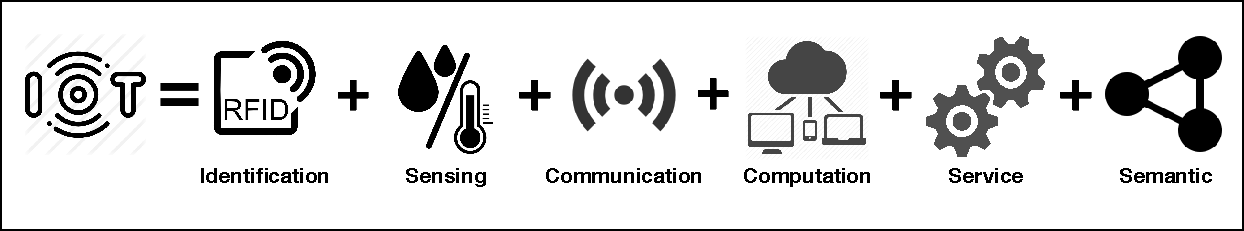
\includegraphics[scale=.75]{Pictures/c2/2-1-IoT-Elements.pdf}
    \caption{The core enabling technologies for the IoT~\citep{Al-Fuqaha:2015}}
    \label{fig:2.2-technologies}
\end{figure}

The previous section discussed the vision and the mission of the IoT. 
The IoT would not be built up from a single technology, but multiple technologies. 
According to ~\cite{Al-Fuqaha:2015}, there have been six core enabling technologies that are required for developing the IoT.
As illustrated in Figure~\ref{fig:2.2-technologies}, the six enabling technologies include: identification technology, sensing technology, communication technology, computation technology, service technology and semantic technology.
In order to provide the better understanding on the IoT, each of IoT technologies is briefly introduced in this section.


\subsection{Identification technologies}
\label{subsec:identification}

The IoT is a system of global interconnected ``things" and IoT applications are typically built based on the integration of these ``things".
In order to ensure the correct integration, the "things" must be uniquely identifiable. 
As the ``things" can be physical entities (e.g. sensors, devices) or virtual entities (e.g. services, computational processes), the technologies for globally identifying of physical and virtual objects are crucial for the development of the IoT.

The identification for physical objects such as computer, mobile devices, networking devices, sensors has already been developed.
The physical objects can be identified by their associated identifier such as a host name, an IP address or URI (Universal Resource Identifier).
The identifiers may contain the additional information of the relationship of physical objects or their locations.
Moreover, the technologies for identifying virtual objects such as services, datastores, web objects, digital documents have also been implemented.
For example, URLs (Universal Resource Locators) has been used for identifying, locating web services, or digital documents can be referenced with DOI(Digital Objects Identifiers).

\begin{table}[ht!]
    \centering
    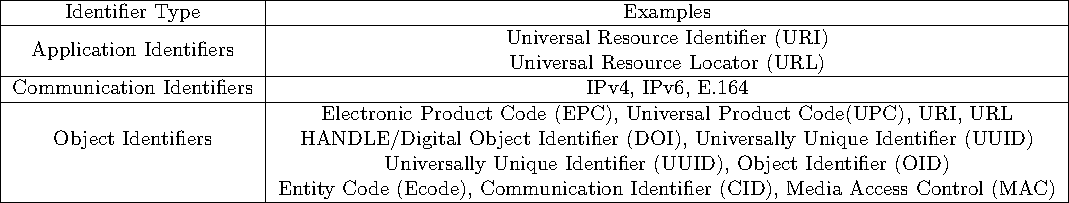
\includegraphics[scale=.85]{Table/2-1-identfication.pdf}
    \caption{Caption}
    \label{tab:IoTIds}
\end{table}

\cite{Presser:2016} reported the available identification methods in the IoT. 
These methods serve different purposes and operate at different layers.
IoT identifiers can be classed into: 
(i) Objects identifiers which are simply used for defining the unique of physical/virtual objects;
(ii) Communication identifiers which are used to uniquely identify connected objects in the context of communications with other objects;
(iii) Application identifiers which are used to identify services, applications. 
The examples of identifiers for the IoT are provided in Table~\ref{tab:IoTIds}

The identification for IoT is composed of three technologies: IoT ID naming, IoT ID addressing and IoT ID discovering~\citep{Presser:2016}.
Naming means assigning labels or attributes to objects or a group of objects to individualise or specify them among larger set of objects.

Addressing is to assigning addresses for connected objects within a communication network.
Addressing also provide the means for mapping of the identifiers at different layers to the communication identifiers.
IoT discovering is the process of locating devices, services or data. 
There are various approaches for the discovery in the IoT, for example, geographic location-based discovery approach~\citep{Dinh:2017}, semantic web-based discovery approach~\citep{Serena:2017}.

---
\nop{
The IoT ID naming technologies have been used including: CID (Communication Identifier), ECODE (Entity Code), HANDLE/DOI
name: OID (Object Identifier) , IPV6, Handle/DOI, BAR CODES and RFID, URIs and UUIDS,
address: DNS (Domain Name Systems), HANDLE
discovery: Resource Discovery in web of things, device abstraction in m2m,

As IoT is a system of interconnected ``things", its applications are typically based on the integration of these ``things".
Similarly to any interactive system, the unique identification of ``thing" is require to ensure the correct integration.
Identification is critically important for any system that requires the interaction between different components. 
The identification of each component in a system is needed to ensure the correct integration of the system.
The IoT could be seen as a global interaction system and its components are users, services, devices and physical objects.
Therefore, ``things" in the IoT must be identified in order to enable such interaction.
    
Due to the continuous increase of the connected devices, providing scalable addressing and identification mechanism is challenging for the IoT. 
The designs of such mechanisms also have to cope to the heterogeneity of the ``things" which could be physical objects or virtual objects. 
Physical objects such as wireless sensors, mobile devices, computers are associated with identifiers such as host names, IP addresses.
Whereas, virtual objects could be identified by the mechanisms, for example, ULRs (Universal Resource Locators) for identifying web services, or DOIs (Digital Objects Identifiers) for referencing digital documents.
The identification for the IoT would be required to address the full range of physical and virtual objects.}




\subsection{Sensor Networks}

%what is sensing
Sensing technologies are the key enablers of the integration of physical world and the virtual world.
Sensors are the electronic devices that can detect events, changes in its environment or measure the quantity of the physical properties.
By converting the signals from physical stimuli into digital form that is readable by machines, sensors allow the IoT understand the environmental characteristics surrounding physical things.

In order to increase the capability of observing the physical world in the IoT, multiple sensors are formed sensor networks.
In the sensors networks, sensors can communicate with each other via wire or wireless connectivity. 
With the better mobility and lower cost, wireless sensors are more attractive for deploying sensor networks~\citep{Sheng:2015}.

%raw data need to be describe

\subsection{Communication}

Communication is the backbone technology of the IoT that connects heterogeneous objects, devices together to provide smart services. 
IoT devices are resource constrained devices, IoT nodes should operate using low power in the presence of lossy and noisy communication links.
This section provides the overview of networking technologies that enable the communication for the IoT.


\subsubsection{Wireless Network Technologies}

%[Low-range]

\textbf{Near Field Communication} is low-range wireless connectivity technology which allows small data to be transmitted over distance of few centimetres. 
Similarly to RFID, NFC transfers data by generating magnetic field and operates over a frequency band of 13.56 MHz.
However, NFC allows both one-way and two-way communications between two devices.
Furthermore, NFC has two operating modes: active and passive.
In active mode, both the sender and the receiver  generating their own fields.
Passive mode is useful for saving energy as only one device generates the field, and the other answers by modulating the existing field.

\textbf{Bluetooth} is the wireless technology that uses short-wavelength UHF radio for exchanging data over short distance.
Compared to NFC, Bluetooth supports broadcasting and provides wider range connectivity with higher frequency and data throughput. 
\textit{Classic Bluetooth} offers enough throughput for data stream application, however, it has several limitations including limited number of nodes in the network.
\textit{Bluetooth Low Energy} or ``\textit{Bluetooth smart}" is advanced over Classic Bluetooth.
It consumes less energy, supports unlimited number of nodes, however, it does not support data streaming and offers lower data rate.
The recent version, \textit{Bluetooth 5.0}, increase the communication range up to 300m and doubles the speed of the low energy connections. 

\textbf{Zigbee} is another low-cost, low-power wireless technology which is based on IEEE 802.15.4 communication protocol.
Compared to Bluetooth or NFC, it offers lower data transferring rate but  much wider communication range.
Depending on power output, outdoors with line-of-sight of Zigbee may range up to 1500m.
Zigbee devices are of there types: Zigbee Coordinator(ZC), Zigbee Router(ZR), Zigbee End Device (ZED).
ZED devices are the simplest devices in Zigbee networks, they just have basic functionalities to communicate with its parent which can be ZC or ZR. 
In a Zigbee network, ZC device is the most capable device whose roles are the root of the network and the bridge to other networks.
Whereas, ZR devices are the intermediate routers for passing data from devices to devices internally. 

\textbf{Z-Wave} is popularised as low-power wireless communication technology for Home Automation Networks.
It covers about 30 meters point-to-point communication, therefor, being widely used in remote applications in smart homes.
Z-wave operates in ISM band around 900MHz and the recent version supports transmission rate up to 200Kbps.

\textbf{Low Power WiFi} is also known as ``WiFi HaLow", which is based on IEEE 802.11ah standard.
The development of WiFi HaLow attempts to extend the range of transmission and to reduce the energy consumption for the WiFi.
Compared to conventional WiFi(IEEE 802.11 b/g/n), the range that HaLow can communicate is doubled.
Wireless sensor networks are the motivated scenarios of HaLow, in which, the devices are energy constrained and require relatively long range connectivity. 

\textbf{Low Power Wide Area Network (LPWAN)}  is a class of the very long range wireless technologies that are suitable for low power application. They can support up to 10 Km distance, however, very low data rate. The technologies in this class include SigFox, LoRaWan and Weightless. 

\textbf{Cellular networks} such as 3G,4G, LTE can provide high-speed connectivity to the Internet for mobile devices. These technologies are based on GSM/UMTS technologies, providing multicasting and broadcasting for fast-travelling devices.
However, they have high power consumption profile.
The under-developing 5G network is expected to be rolled out by 2020 which targets high data rate, reduced latency, energy saving, cost reduction, higher system capacity, and massive device connectivity

\begin{table}[ht!]
    \centering
    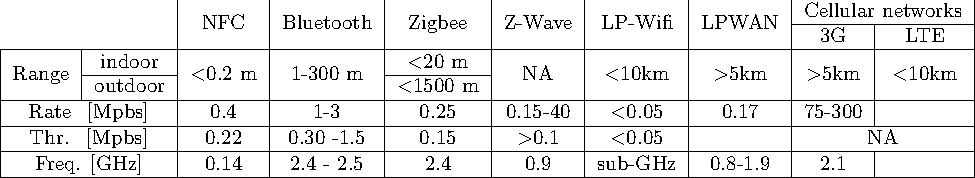
\includegraphics[scale=.95]{Table/2-2-wireless.pdf}
    \caption{Caption}
    \label{tab:my_label}
\end{table}

\subsubsection{Network Protocols}

The full conventional IP suite is very complex and requires a large amount resource on the connecting devices.  
Therefore, the Internet Engineering Task Force(IETF) and IPSO Alliance have been developing alternatively protocols for resource constrained devices in the IoT~\citep{Ishaq:2013, alliance:2011}. 

The IEEE 802.15.4 protocol is designed as a standard for physical and link layers for low-rate wireless personal area networks(PL-WPAN).
To cope with resource constrained environment, it comes with a small frame size, low bandwidth and low transmit power.
Therefore, this protocol can support low power consumption, low data rate, low cost and high message throughput for devices that need a long battery life.

In the Internet layer, IPv6 can provide larger IP addressing space for the large number of IoT devices. 
However, IPv6 was initially developed not thought to be suitable for low-power wireless links.
6LoWPAN which is an acronym of IPv6 over Low-Power Wireless Personal Area Networks provides an adaption layer that allows IPv6 packet to be transmitted over IEEE 802.15.4 links.
To connect with the Internet, 6LoWPAN networks requires a gateway to convert IPv6 and IPv4 as today’s deployed Internet is mostly IPv4. 
The header of IPv6 is lager than the \textit{maximum transmission unit}(MTU) of 802.15.4, 6LoWPAN proposes the following optimisation:
(i) Compressing the header of IPv6 by deleting some of the fields that can be derived from link level and be shared across packets;
(ii)Fragmenting the IPv6 packets into small packets;
(iii) Forwarding to link-layer to support routing and multi-hop delivery.

In the Network layer, the IETF Routing over Low Power and Lossy Networks(ROLL) working group standardised a routing protocol based on IPv6 for resource constrained node called RPL.
RPL was optimised to meet only the minimal routing requirements over lossy links while supporting from simple to complex routing topology.


%[rewrite]
The conventional Internet often uses HTTP application protocol, however, HTTP is not suitable for IoT resourced constrain nodes.
The \textit{IETF Constrained RESTful Environments} (CoRE) working group created \textit{Constrained Application Protocol} (CoAP) that simplifies the HTTP to meet the resource constrained environment of the IoT. 
CoAP also uses REST principles on top of HTTP functionalities, utilises methods such as GET, PUT, POST and DELETE to perform Create, Retrieve, Update and Delete (CRUD) operations.
Therefore, CoAP can be considered as an alternative version of HTTP.
However, to be suitable for resource constrained applications, CoAP is bound UDP rather than TCP.
Unlike HTTP, CoAP uses  EXI (Efficient XML Interchanges) data format, which is space efficient comparing to plain text HTML/XML.
A typical CoAP message can be between 10 to 20 bytes.

\textit{Message Queue Telemetry Transport} (MQTT) is application protocol for messaging developed by IBM.
MQTT is built on top of TCP with a publish/subscribe pattern.
It consists of three components: subscriber, publisher and broker.
The publisher and the subscriber are registered to send/receive data to/from a specific topic.
The broker handles data transmission between publisher and subscriber that are registered to the same topic.
The connection operation uses a routing
mechanism (one-to-one, one-to-many, many-to-many) and enables
MQTT as an optimal connection protocol for the IoT
and M2M.
The initial version of MQTT only operates over TCP which cannot be used with all types of IoT devices, and the topic name 
is represented in text that increases its overhead.
The latter version of MQTT-SN was optimised the earlier version for sensor networks and constraint devices.
It supports UDP mapping and indexing on topic names. 
It is designed for small code footprints and can be implemented in devices with less than 64kb of RAM.

\subsection{IoT hardware and software}

Computational units are the atomic components of the IoT, various hardware platforms and software were developed to run IoT applications. 
Recent advances in the technologies of embedded processor have increased the processing capabilities of IoT devices.
Many devices now can be deployed in network via different communication technologies.
Based on the computational capability, IoT devices can be categorised into two categories~\citep{Hahm:2016}: \textit{low-end}  and \textit{high-end}.
The low-end IoT devices are very constrained in terms of resources including energy, CPU(less than 100MHz) and memory capacity (less than 100 kB).
Popular examples of devices in such category include 
Arduino~\footnote{https://www.arduino.cc/}, 
Zolertia~\footnote{https://zolertia.io/}, 
OpenMote node~\footnote{http://www.openmote.com/}, etc.
The second category consist in high-end IoT devices, which includes single-board computer such as Raspberry Pi~\footnote{https://www.raspberrypi.org/}, 
Beagle Bone board~\footnote{https://beagleboard.org/bone} or 
smartphones.
The high-end devices are more powerful than the low-end devices.
They have enough resources and adequate characteristic to run software based on tradition operating systems such Linux or BSD. 


Furthermore, many IoT software platforms are utilised to provide programming frameworks, programming frameworks, ma-chine-to-machine (M2M) integration, data and device management, security and storage, and protocol translation. 
Several real-time operating systems were specifically developed for the limited resource devices such as low-end IoT devices.
The list of the available of operation systems for IoT can be found in~\citep{Hahm:2016}.
Among of these operating systems, the Contiki~\citep{Biljana:2017}, TinyOS~\citep{Amjad:2016}, LiteOS~\citep{Vanitha:2010} and RiotOS~\citep{Baccelli:2013} have been used widely in many IoT scenarios. 


Moreover, cloud infrastructures are another important computational resources for the IoT~\citep{Botta:2016}.
The cloud computing has been a mature technology and has been considered as an unlimited capabilities storage and processing power.
The IoT also has been integrated with the cloud computing that introducing the \textit{``Cloud of Things"}~\citep{Jiehan:2013} or the ~\textit{``IoT Cloud"}~\citep{Truong:2015}.
These cloud-based systems allow IoT data to be uploaded into cloud where data is processed, and the requesting results are sent back to the IoT devices or IoT applications.
There many cloud platforms and frameworks available to host IoT services such as IBM Bluemix IoT platform~\footnote{https://console.ng.bluemix.net/}, Oracle IoT cloud~\footnote{https://cloud.oracle.com/iot} or Microsoft research Lab of Things~\citep{Brush:2013}.

\subsection{Services}

There four classes of IoT services that are available in many researches references: ~\textit{Identity-related Services}, \textit{Information Aggregation Services}, ~\textit{Collaborative-Aware Services} and ~\textit{Ubiquitous Services}~\citep{Mohammed:2015}.
Identify-related services are the most basic but important services. 
As presented in Section~\ref{ss:identification}, every device that connected to the IoT network has to be identified.
Therefore, every application, service in the IoT requires this type of services to identify the things that are involving. 
Raw sensory data is collected, processed and reported to the to IoT application using Information Aggregation services. 
Collaborative-Aware services are the smart services that can make smart decisions.
These services are often built on top of the Information Aggregation services and able to react accordingly to information provided by the Information Aggregation services.
Ubiquitous services aim to provide Collaborative-Aware services to anyone, from anywhere, at anytime.
The ultimate goal of all IoT applications is to enable the Ubiquitous services.
However, this goal is not easy to achieve, most of the existing applications provide identity related, information aggregation, and collaborative-aware services~\citep{Al-Fuqaha:2015}.
A \textit{smart city}~\citep{Jin:2014, Zanella:2014} which could be seen as an application of ubiquitous services, aims to improve the quality of life in the city by making it easier an more convenient for the residents to find information of interest.

\subsection{Semantic}

%[rewrite]
Semantic in the IoT refers to the ability to extract knowledge smartly by different machines to provide the required services.
Knowledge extraction includes discovering and using resources and modeling information.
Also, it includes recognizing and analyzing data to make sense of the right decision to provide the exact service [62]. 
Thus, semantic represents the brain of the IoT by sending demands to the right resource. 
This requirement is supported by Semantic Web technologies such as the Resource Description Framework (RDF) and the Web Ontology
Language (OWL).
In 2011, the World Wide Web consortium (W3C) adopted the Efficient XML Interchange (EXI) format as a recommendation [63].
EXI is important in the context of the IoT because it is designed to optimize XML applications for resource-constrained environments. 
Furthermore, it reduces bandwidth needs without affecting related resources such as battery life, code size, energy consumed for processing, and memory size. 
EXI converts XML messages to binary to reduce the needed bandwidth and minimize the required storage size.



%=======================================================================================
\section{IoT Architectures}
\label{sec:architecture_of_iot}
\lhead{2.3 IoT Architectures}
%=======================================================================================


In the early stages of research in this areas, three-layer architecture as show in Figure~\ref{fig:2.3-iot-architecture}a was proposed~\citep{Wu:2010,Yang:2011}. 
The IoT could be built up with three layers defined as \textit{perception layer}, \textit{network layer} and \textit{application layers}:

\begin{itemize}[noitemsep,nolistsep]
\item Perception layer: 
This layer is also know as physical layer or sensor layer and is the bottom of the IoT architectures. 
This layer has sensors, actuators for observing and gathering physical information of their surrounding environment.
Information collected from this layer, then, is transmitted to the network layer.
Devices in the layer also perform some collaboration tasks with each other via short range networks.

\item Network layer: 
This layer is responsible for connecting ``Things". 
Its main feature is to transmit information between long distance. 
It comprises of communication and integration networking devices that function data routing, transmission to different IoT nodes, systems using recent networking technologies Wifi, LTE etc.
This layer also includes computing platform that takes part in processing information.
For example, the IoT gateways~\citep{Guoqiang:2013} take place in this layer serving as the mediators for the network interoperating, data aggregating, filtering and transmitting for different IoT nodes.
The other computing platforms such as clouds or expert systems may also involve in this layer, 
therefore, the network layer not only has the competence of network operation, but also enhance the competence of information operation.

\item Application layer:
This layer is responsible for discovering and delivering services to IoT users.
The application layer is a connection for the IoT and domain-specific systems, for example, smart home~\citep{Biljana:2017}, smart cities~\citep{Gaur:2015}, smart health~\citep{Catarinucci:2015}.
\end{itemize}


\begin{figure}[ht!]
    \centering
    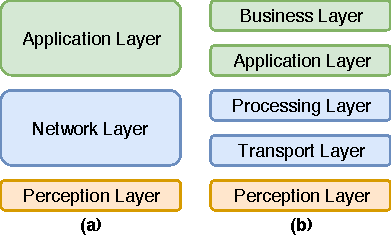
\includegraphics[scale=1.5]{Pictures/c2/2-2-IoT-architectures}
    \caption{Caption}
    \label{fig:2.3-iot-architecture}
\end{figure}


The three-layer architecture covers enough the main idea of the IoT, however, researchers often work toward the finer aspects of the IoT~\citep{Sethi:2017}.
Therefore, many more layered architecture were proposed to clarify the network layer and application of the three-layer architecture.
In the recent literature, the five-layer architecture~\citep{Wu:2010,Khan:2012} has been proposed with added \textit{transport layer}, \textit{processing layer} and \textit{business layer} as shown in Figure~\ref{fig:2.3-iot-architecture}b:
\begin{itemize}[noitemsep,nolistsep]
\item Transport layer: Differently from the network layer of the three-layer architecture, the transport layer only takes responsibility of transmission data from perception layer to the processing layer. It only includes networking technologies in this layer.

\item Processing layer: This layer is also known as middleware layer which is responsible for storing and processing data. Cloud computing and ubiquitous computing are the primary technologies in this layer.

\item Business layer: This layer manages the whole IoT system including applications, business and profits models. The success of the IoT not only depends on the advance of the updated technologies but also the innovation and reasonable of business model.

\end{itemize}

From system architecture perspective, the IoT systems can be classified into cloud-based systems and edge-based systems depending on where the processing layer take places.
In some architectures, for example, Cloud of Things~\citep{Jiehan:2013} or IoTCloud~\citep{Truong:2015}, data is processed in a large centralised fashion by cloud infrastructure.
On the other hand, in edge-based architecture, sensors, gateways, edge devices take part in data processing. 


\subsection{Cloud-based IoT Architecture}

%[Cloud infrastructure]
The widely accepted definition of cloud computing was phrased by the Nation Institute of Standard and Technologies(NIST)~\citep{Mell:2012} as 
‘‘Cloud computing is a model for enabling ubiquitous, convenient, on-demand network access to a shared pool of configurable computing resources (e.g., networks, servers, storage, applications, and services) that can be rapidly provisioned and released with minimal management effort or service provider interaction’’.
The cloud is composed of four layers: datacenter, infrastructure, platform, and application~\citep{Zhang:2010}.
Each of them can be seen as a service, for example, platform as a service (PaaS), infrastructure as a service(Iaas).
There are twofold benefits that the cloud computing can bring to the IoT: the virtually unlimited capability and resources~\citep{Zhang:2010}, and the scalable service delivery.

%[Cloud IoT Integration]
The integration of the could computing and the IoT was derived from the ideas that the cloud could be a bridge between IoT data collection, data processing, services delivering, filling the gaps of the lack of storage, computation and communication of IoT devices~\citep{Botta:2016}.
~\cite{Rao:2012} proved that the cloud can be an inexpensive and effective solution for things management from anywhere, at any time by using customised portals and built-in apps.
The huge amount of data produced by the IoT can be stored and processed by the datacenters which can on-demand storage capacity and processing capabilities that~\citep{Parwekar:2011}.
The ``everything as a service" paradigm of cloud computing can be applied on ``Things" introducing the ``\textit{Sensing as a Service}" paradigm~\citep{Zaslavsky:2013} or ``\textit{Things as a Service}" paradigm~\citep{Christophe:2011}.

\begin{figure}[ht!]
    \centering
    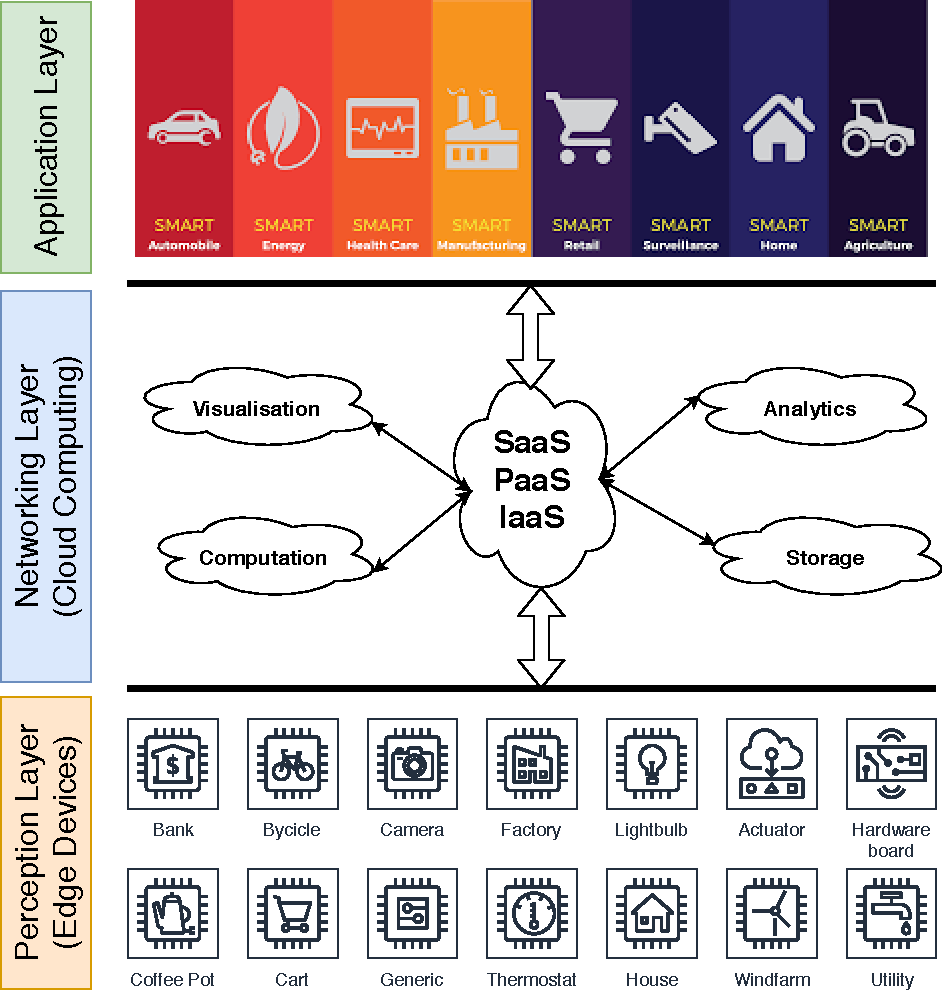
\includegraphics[scale=.65]{Pictures/c2/2-3-Cloud-based-architecture.pdf}
    \caption{Could based architecture}
    \label{fig:2.3.2-cloudIoT}
\end{figure}

Figure~\ref{fig:2.3.2-cloudIoT} illustrates an overview of architecture for the cloud of things. 
Data generated from the perception layer is sent through the communication layer to the cloud.
According to the requirements of the services, cloud provides storage and computation for data storing, data processing or data analysing. 
Once the service is created, it is made available from cloud for other applications to access.

There have been many 


\subsection{Fog/Edge-based IoT Architecture}

Although cloud infrastructures have been efficient for processing IoT data as computational resources on the cloud outclasses that of IoT devices at the edge, cloud-based IoT systems would encounter the issues related to network latency and traffic~\citep{Bonomi:2012,Zhang:2015,WShi:2016}.
The end devices in the IoT are not only data consumers as in cloud computing paradigm but data producers.
Therefore, the common approaches of directly connecting IoT devices and pushing IoT data to the cloud may have several disadvantages~\citep{Zhang:2015}.
The increasing of the number of the IoT devices means the quantity of produced IoT data is raising quickly.
Most of the data can be discarded immediately after being processed.
Hence, in these centralised systems, the bandwidth would be overwhelming and might be wasted.
Furthermore, pushing data into cloud will dominate upstream network traffic, meanwhile, broadband networks have more downstream bandwidth than upstream bandwidth.
Moreover, some IoT applications might require very quick response time, unfortunately, cloud-based solution may lead these applications to be less operable due to unexpected network latency.
In additional, IoT data might contain sensitive information from the sensors that are implanted surrounding us.
Cloud-based systems create more privacy and security concerns as centralised storage are out of users' control.
To address the issues of network overhead and network latency, and to improve the scalability for the IoT, the recent fog/edge based IoT architecture has been proposed~\citep{Bonomi:2014,Salman:2015}. 
As illustrated in Figure~\ref{fig:2.3.3-egdeIoT}, in fog/edge based system architecture, edge devices take part in data storing and data processing.

\begin{figure}[ht!]
    \centering
    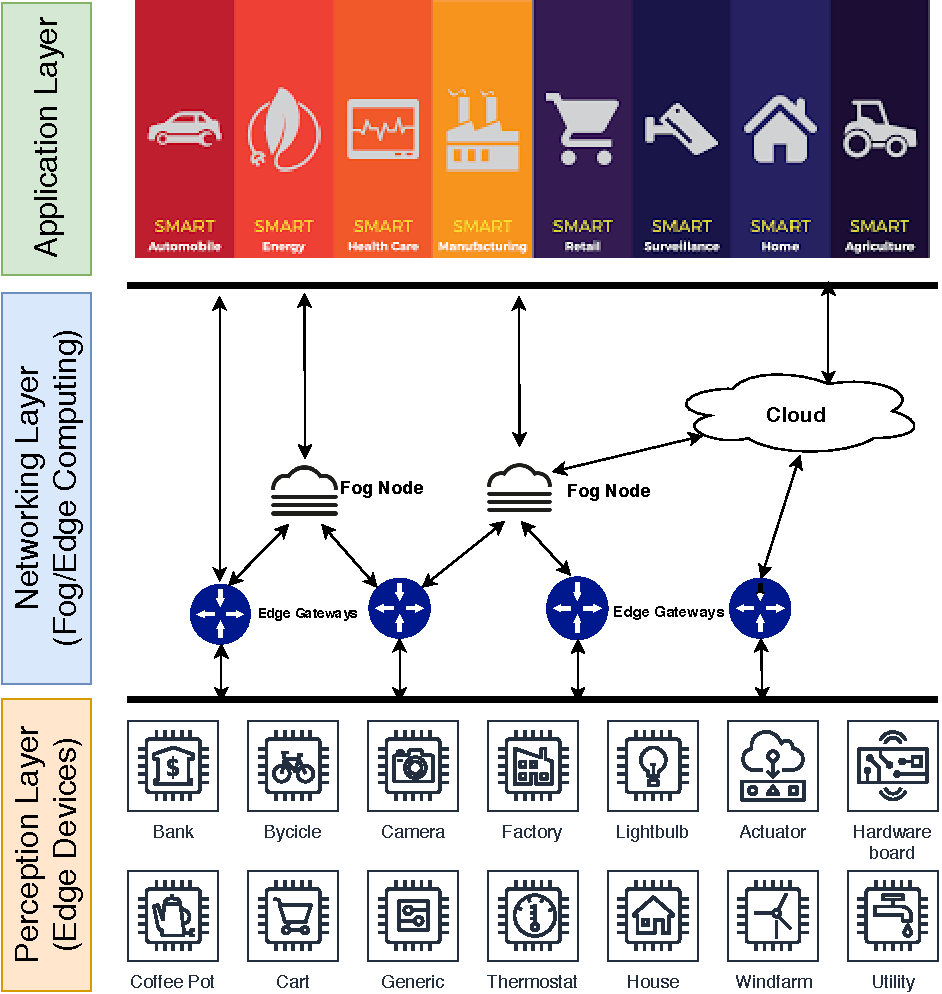
\includegraphics[scale=.65]{Pictures/c2/2-4-Edge-based-architecture.pdf}
    \caption{Caption}
    \label{fig:2.3.3-egdeIoT}
\end{figure}

\cite{Bonomi:2012} from Cisco stated that ``\textit{fog computing} is a highly virtualised platform that provides compute, storage and networking services between end devices and traditional Cloud computing Data Centres, typically, but not exclusively located at the edge of the network".
Meanwhile, \cite{WShi:2016} explained that ``\textit{edge computing} refers to the enabling technologies allowing computation to be performed at the edge of the network, on downstream data on behalf of cloud services and upstream data on behalf of IoT services".
Both fog computing and edge computing aim to provide the computation, storage, communication, services capabilities to the edge of network.

\cite{WShi:2016} defined the ``edge" as ``any computing and network resources along the path between data sources and cloud data centres".
In fog/edge based IoT architecture (see. Figure~\ref{fig:2.3.3-egdeIoT}),the fog/edge layer may include large number of edge/fog nodes which usually are routers, gateways, switchers, base stations or specific fog servers that are placed between end devices and cloud. 
Fog/edge nodes can be static at a fix point such as street light, house, offices or mobile on a moving objects such as smart phones or connected vehicle~\citep{Bonomi:2014}. 
These fog/edge nodes that have capabilities to compute, transmit and store the temporary data.
The end users can connect to these fog/edge nodes to obtain applications, services.
As fog layer is placed close to end users, edge/fog layer could support latency-sensitive applications, services.
Moreover, in the situation that more powerful computing and storage capabilities is required, fog/edge node can be connected to cloud. 



Both fog computing and edge computing paradigms is to decentralise and distribute data processing and storing from cloud to edge networks, these two terms are often used interchangeably.




For edge computing and fog computing, their architectures are hierarchical, decentralized, and distributed, which is different from centralized cloud computing architecture. 
Their service locations are the proximity to end users.
Edge computing is located in edge devices,while fog computing is located in network edge devices, which is single network hop or few network hops away from the edge. 
Their resources(e.g., computing, communication and storage resources) and computation and storage capabilities are limited by comparing with cloud computing, and edge computing is more limited than fog computing.
Because the resources and service capabilities of network edge devices are relatively stronger than edge devices. 
Moreover, these two computing paradigm have mobility support for end users. 
Because most services are provided locally, it is essential to take the existence of mobile devices into consideration. 
They also support the scalability of the whole ecosystem. 
The reason is that a large number of wide-spread and geo-distributed nodes are available if the situation requires them,including the nodes located at a certain site, neighboring nodes, or even the nodes situated at more remote geographical locations (Romanet al.,). 
Furthermore, they are highly virtualized computing platforms.
The nodes and networks are not always physical, while virtual sensor nodes and virtual sensor networks are also used for implementing various services (Aazam and Huh, 2014Aazam and Huh, 2014). 
The virtualized service mechanisms can be provided by them.

Obviously, even if they have the same goal, there are still some underlying differences between edge computing and fog computing. 
In edge computing, edge devices cannot implement multiple IoT applications, because the limited resources will result in resource contention and increase processing latency. 
While fog computing can overcome these limitations felicitously and avoid resource contention at the edge by seamlessly integrating edge devices and cloud resources. 
It coordinates the use of geographically distributed network edge devices and leverages the cloud resources to balance the use of resources and improve the utilization (Dastjerdi and Buyya, 2016). 
Furthermore,edge computing pays more attention to the things level, while fog computing focus more on the infrastructures level.

For edge computing and fog computing, their service locations are the proximity to end users. However, Edge computing is located in edgedevices, while fog computing is located in network edge devices, whichis single network hop or few network hops away from the edge. Edgecomputing platform usually tends to be constrained devices, whichbattery or storage capacities often are the limiting factors. When themultiple IoT applications need to be handled, this will result inresource contention and increases processing latency (Dastjerdi andBuyya, 2016). So the resource contention of edge computing is moreserious than fog computing. Moreover, edge computing focus more onthe things level, while fog computing focus more on the infrastructurelevel


\begin{table}[ht!]
    \centering
    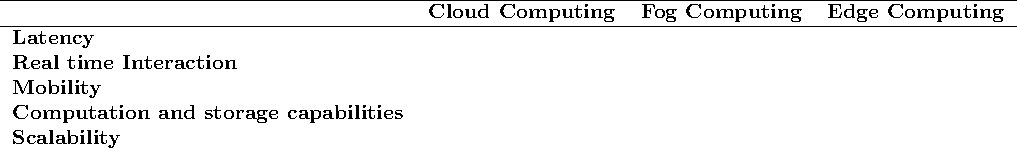
\includegraphics[scale=.75]{Table/2-3-edge-fog-cloud.pdf}
    \caption{Caption}
    \label{tab:my_label}
\end{table}

The edge computing has been emergent and benefit for the IoT~\citep{Yu:2018}. 
There have been several early results that demonstrated the benefit of applying edge computing. 
Face recognition application could run 4 times faster by moving computation from cloud to edge~\citep{Yi:2015}.
Using cloudets for offloading computing tasks did not only reduce the response time for wearable cognitive assistant but also save 30$\%$ to 40$\%$ energy consumption~\citep{Ha:2014}. 
However, computing nodes often have less computational resource and networking capability. 
This poses a challenge for the computing tasks to be physically moved to the edge nodes.



\section{Summary}

IoT developments during recent years have been characterized by
attributes that can be “labelled” the 6As: Anything (any device), to be
transferred from/to Anyone (anybody), located Any place (anywhere), at
Any time (any context), using the most appropriate physical path from Any
path (any network) available between the sender and the recipient based
on performance and/or economic considerations, to provide Any service
(any business). The IoT paradigm is evolving and entire IoT ecosystems
are now built upon innervation elements known as the 6Cs: Collect (het-
erogeneity of devices of various complexities and intelligence, that enhance
the real-time collection of data generated from the connections of devices
and information), Connect (ubiquitous distributed connections of heteroge-
neous devices and information, where the connections are the foundational
component of the IoT), Cache (stored information in the distributed IoT com-
puting/processing environment), Compute (advanced processing and com-
putation of data and information), Cognize (information analytics, insights,
extractions, real-time AI processing and Create (the creation of new interac-
tions, services, experiences, business models and solutions). This is illustrated
in Figure 3.1






















\nop{

%==================================================================================================
\section{The Semantic Web technology}
\label{s:sw}
%==================================================================================================

According to World Wide Web Consortium(W3C), the Semantic Web technologies aim to ``provide a common framework that allows data to be shared and reused across application, enterprise, and community boundaries".
The Semantic Web community has developed a suite of standards and technologies to formally describe the semantics, support automated reasoning on web data.
As we mentioned in Section~\ref{ss:stiot}, such technologies developed by the Semantic Web are potentially the solutions to data integration, semantic interoperability, context awareness and knowledge transformation in the IoT.
This section introduces the core technologies of the Semantic Web that including Resource Description Framework~\citep{Lassila:1999},RDF schema~\citep{Dan:2004}, Web ontology language~\citep{Guinnes:2004} and SPARQL query language~\citep{Eric:2008}.

%===================================================
\subsection{RDF Data Model}
\label{ss:rdf}
%===================================================
A \textit{data model} is an abstraction that is used to represent the information of real world entities.
It defines how the properties and relations of the entities are represented, and the operations can be performed on the information.
Data models can be categorised as relational, tree and graph based. 

\begin{figure}[ht!]
	\centering
	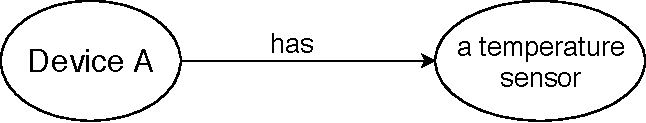
\includegraphics[scale=.65]{c2/2-2-SimpleTriple.pdf}
	\caption{A triple}
	\label{fig:2.2-simpleTriple}
\end{figure}

RDF data model is a graph-based data model. 
Its design is based on the idea that things can be represented by statements in a simple manner of triples. 
The statement is similar to a simple sentence that has subject, verb, object.
The triple is composed of three elements: a subject, a predicate and an object that represent the statement.
For example, the sentence "Device A has a temperature sensor" can be expressed as a triple as follows: ``Device A" is the subject, ``has" is the predicate and ``a temperature sensor" is the object.
The statement can be visually expressed in Figure~\ref{fig:2.2-simpleTriple}

An RDF triple is built from \textit{IRIs} (International Resource Identifiers), \textit{literals} and \textit{blank nodes} which are also called \textit{resources}~\citep{Cyganiak:2014}. 
RDF triple can be formally define as follow:
``An RDF triple is a tuple (S, P, O) $\in$ (I$\cup$B)  $\times$ I $\times$ (I$\cup$B$\cup$L), where S is the subject, P is the predicate and O  is the object and I, B and L are used to represent IRIs, blank nodes and literals respectively."

The IRI is a unique identifier that presents a thing or a concept.
For example, the IRI for representing the device A in the previous example might be ``\textit{http://insight.org/device/A}". 
The IRI ``\textit{http://insight.org/sensor/temperature}" can refer to the concept of ``temperature sensor".
Literals are used to represent value data types such as numbers, booleans or strings. 
A literal might be a simple string such as ``a temperature sensor", or with a optional language tag, ``a temperature sensor"$@$en, 
denoting the language (English), or with an IRI, ``temperature sensor"{\symbol{94}\symbol{94}}\textit{http://www.3.org/2001/XMLSchmea$\#$String}, assigning the datatype (String). 
The blank node (B-Node) is used to refer to a concept with giving it a name. 
The usage of the blank will be explained shortly in the later example.

In an RDF triple, the subject is an IRI or a blank node as it must refer to a concept. 
The object can be an IRI, a blank node or literal. 
The predicate is guaranteed to be an IRI denoting a bi-relationship between the two resources. 
Figure~\ref{fig:2.3-SimpleRDFTriple} shows the presentation of the previous example statement as an RDF triple.

\begin{figure}[ht!]
	\centering
	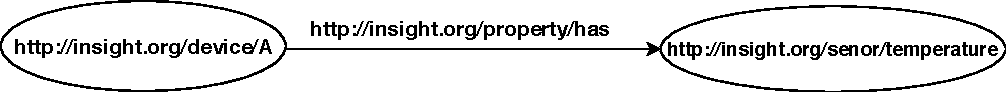
\includegraphics[scale=0.75]{c2/2-3-SimpleRDFTriple.pdf}
	\caption{An RDF Triple }
	\label{fig:2.3-SimpleRDFTriple}
\end{figure}

An RDF document is a set of RDF triples.
The RDF document can be represented as a directed graph as illustrated in Figure~\ref{fig:2.4-SimpleRDFGraph}.
The nodes represent subjects and objects, the predicates are represented by labelled edges with the direction from subjects to objects. 
Therefore, RDF documents are also called RDF graphs.

\begin{figure}[ht!]
	\centering
	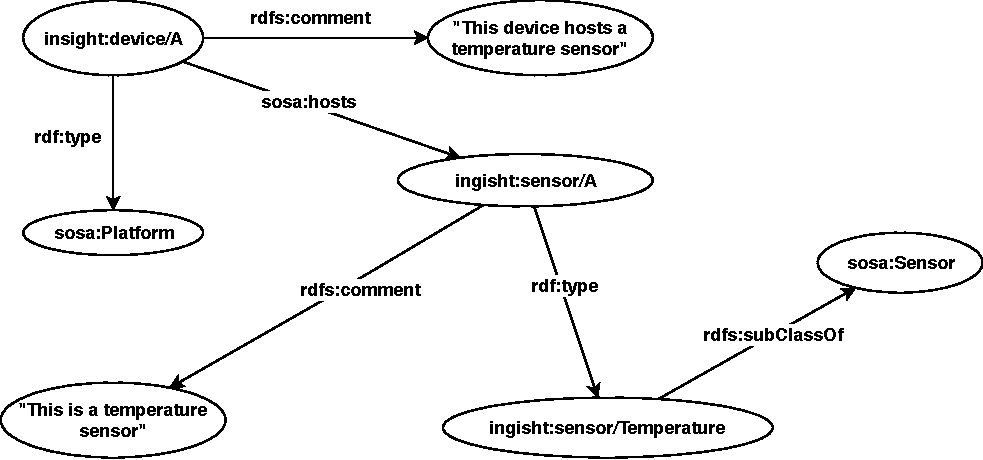
\includegraphics[scale=0.65]{c2/2-4-SimpleRDFGraph.pdf}
	\caption{RDF document describing device A as an RDF Graph.}
	\label{fig:2.4-SimpleRDFGraph}
\end{figure}

\textit{Vocabularies} are used to define concepts and their relations that related to a specific domains. 
For example, to describe people and their relationship, FOAF~\citep{Dan:2010} can be used.
SSN~\citep{Armin:2017} is another RDF vocabulary used for describing devices, sensors.
An RDF vocabulary is a collection of IRIs that used for describing schema and instance data.
The IRIs in an RDF vocabulary are often created with a common substring in the beginning which is called \textit{namespace} of an vocabulary.
For convenience, prefixes can be used to shorten the string representation of these IRIs.
Figure~\ref{fig:2.4-SimpleRDFGraph} illustrated the RDF document describing the devices A from the previous example.
RDFS vocabulary~\citep{Dan:2014}, which is used to defined and documented additional RDF vocabularies, and the SSN vocabulary are used.
For simplicity, prefixes are use the replace the namespaces and the list of prefixes and their corresponding namespace is shown in Listing~\ref{lst:prefixes}.

\vspace{5mm}
\begin{lstlisting}[language=sparql,
  				   captionpos=b,
                   label={lst:prefixes},
                   caption={Prefixes}]  
rdf  : <http://www.w3.org/1999/02/22-rdf-syntax-ns#>
rdfs : <http://www.w3.org/2000/01/rdf-schema#>
sosa : <http://www.w3.org/ns/sosa/>
geo  : <http://www.w3.org/2003/01/geo/wgs84_pos#>
insight : <http://insight.org/>
\end{lstlisting}


The flexible and expressivity of triple lead RDF data model become a great ideal to deal with the dynamic and heterogeneity of the IoT.
RDF  provides both ability to specify concept and ability to link different concepts together.
This enables heterogeneous IoT data to be update and integrated with extremely low effort.

\begin{figure}[ht!]
	\centering
	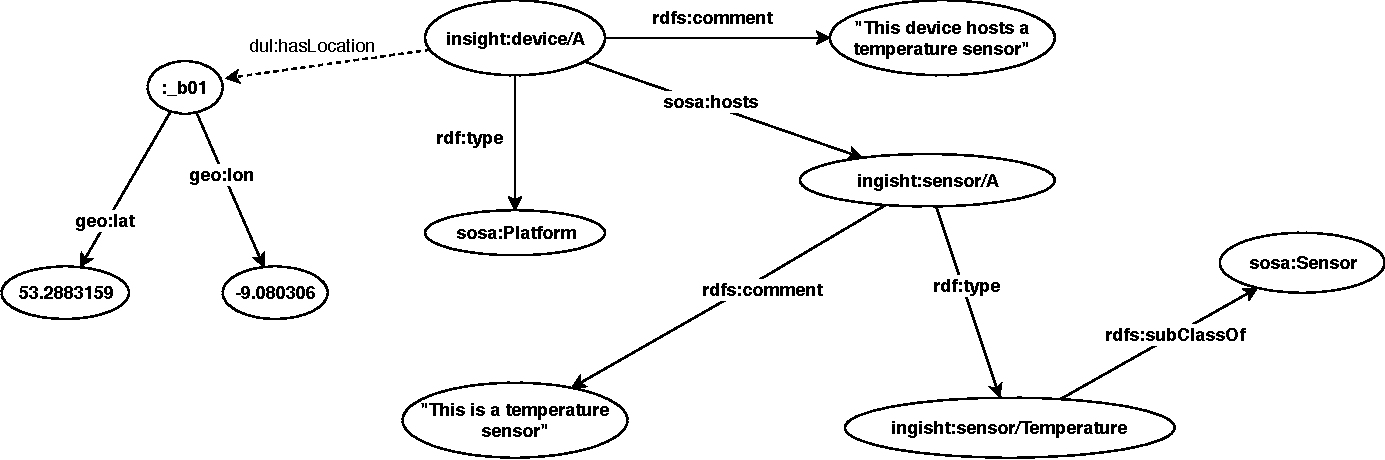
\includegraphics[scale=0.65]{c2/2-5-RDF-integration.pdf}
	\caption{Example of integration RDF graph describe device and RDF graph describing geographic coordinates}
	\label{fig:2.5-integration}
\end{figure}

As a graph data model, to represent information, RDF does not require a predefined data schema as relational databases does.
New type of information, new concept can be introduced without the need of updating data schema.
For example, to give the device A a location requires an integration of the RDF graph from Figure~\ref{fig:2.4-SimpleRDFGraph} with another RDF graph that describes the geographic coordinates.
In Figure~\ref{fig:2.5-integration}, the latitude and longitude values can be added to the RDF graph without introducing what are they.
The machine can understand via the vocabulary that is used to describe the values.
The integration is done by adding a triple to say that device A has located at a point which has the latitude, longitude values as in the figure.
This is much easier than realigning the data schema in case using common relational data model. 
In this example, the location is presented as a blank node as it does not have to be an IRI.

RDF data model allows data to be reusable and shareable.
The same vocabularies can be used in different applications, systems from different domains to describe the same thing.
For example, the vocabulary describing coordinates in a geographic application can be used to describe the location of the device.
Further more, with inferencing (see Section~\ref{ss:inference}), new relationships or concepts can be discovered from the the base relationship found in dataset.
This helps machine to determine if different vocabularies were used to describe the same concept.
In the previous example, the sensor ``\textit{insight:sensor/A}" is defined as ``\textit{a temperature sensor}" using IRI ``\textit{insight:sensor/Temperature}".
By defining ``\textit{insight:sensor/Temperature}" is the subclass of ``\textit{sosa:Sensor}", machine can understand that ``\textit{insight:sensor/A}" also refers to a sensor.
Thus, ``\textit{insight:sensor/A}" is understandable and discoverable as a sensor by another systems or applications that are using SSN vocabulary.

\textit{Linked Data} is an approach for publishing and consuming structured data on the Web using RDF data model.
The principles of Linked data include: (i) Using URIs for naming things; (ii) Using HTTP URIs to enable the look up on things; (iii) Describing the information of the URIs using RDF data; (iv) Including the links to other URIs, so that they can discover more things. 
The same principles can be applied for publishing and consuming IoT data, for example, sensor data~\citep{Patni:2010} or stream data~\citep{Sequeda:2009}.
Linked Data can make data linkable and discoverable thus becomes an efficient solution for the fragmentation issue in the IoT.
RDF data model provides a flexible way to describe things and their relationship, such as devices, observations or measurements. 
RDF vocabularies and inference allow semantics, knowledge to be shared crossing devices, systems and platforms. 
Using Linked Data principles and RDF data model could enable the semantic interoperability for the IoT in the global scale~\citep{Le-Phuoc:2018}.

%===================================================
\subsection{Inference}
\label{ss:inference}
%===================================================

As we mentioned in the previous example, the Semantic Web technologies do not only provide RDF data model to describe concepts and theirs relationships but also the ability to discover new relationships from the given dataset.
This ability is known as inference.
\textit{RDFS}(RDF schema)~\citep{Dan:2004} and \textit{OWL}(Ontology Web Language)~\citep{Guinnes:2004} are the two standards to create vocabularies that enables the inference.

RDFS is derived from RDF by adding some basic constructs to allow the inferencing on the type of things and properties of things.
RDFS is added classes and subclasses to specify different concepts and to describe if two concepts are related.
As shown in the example (see Figure~\ref{fig:2.5-integration}), the device and the sensor are differentiated by the class ``\textit{sosa:Platform}" and ``\textit{insight:sensor/Temperature}". 
The additional triple that says the type ``\textit{insight:sensor/ Temperature}" is a subclass of the type ``\textit{sosa:Sesnor}" infers that the sensor also has type ``\textit{sosa:Sesnor}".
The further additional features are property domains and ranges.
The domains of a property state that any subject that has this property is an instance of a specific class or set of classes.
The ranges of a property define the specific classes (types) that its object can be.

OWL provides more inferencing capability. 
OWL enables the ability to share not just information, but vocabulary.
For example, OWL includes ``\textit{owl:sameAs}" to state if two classes or two properties are the same.
With OWL supporting, two systems that do not use the same vocabulary to publish RDF data might be able to understand and process data the other. 

%===================================================
\subsection{SPARQL Query}
\label{ss:sparql}
%===================================================

SPARQL has been standardised as the query language query RDF data by the the World Wide Web Consortium~\citep{Eric:2008}.
To query graph-based data, SPARQL is designed as a graph-matching query language.
The graph pattern in a SPARQL query can be simple with a single triple pattern of very complex.
Given an RDF graph G and a query Q that consists of a graph pattern, the values obtained form the matching of the pattern against G are formed the answer.

A triple pattern is similar to an RDF triple in which subject, predicate, object could be a variable.
A set of triple pattern forms a basic graph pattern. 
Listing~\ref{lst:SPARQL1} is showing Q1, an example of a SPARQL SELECT query with a simple graph pattern containing a triple pattern.
The query asks for the list of the sub-systems that are hosted on the Device A.

\vspace{5mm}
\begin{lstlisting}[language=sparql,
  				   captionpos=b,
                   label={lst:SPARQL1},
                   caption={Q1 - SPARQL Query with a graph pattern}]  
PREFIX sosa    : <http://www.w3.org/ns/sosa/>
PREFIX insight : <http://ingisht.org/>

SELECT ?subSystem WHERE
{ 
  <insight:Devcie/A> sosa:hosts ?subSystem.
}    		
\end{lstlisting}


A basic graph pattern matches against a RDF graph when the variables can be replaced by values from the graph and form a subgraph of the graph.
For example, the IRI ``\textit{insight:sensor/A}" is replaced the variable ``\textit{?subSystem}" to form a subgraph of the RDF graph in Figure~\ref{fig:2.4-SimpleRDFGraph}.
This value is the answer of the query Q1 against RDF graph in Figure~\ref{fig:2.4-SimpleRDFGraph}.

A more complex may contains more than one basic graph pattern.
A resultant RDF subgraph can be further queried or joined with the results of other basic graph patterns to answer the query.
The query Q2 in Listing~\ref{lst:SPARQL2} asks for a list of subsystems on the device A that are temperature sensors.
The query contains two basic graph patterns, the first pattern asks for the subsystem on the device A and the second pattern asks if its is a temperature sensor.

\vspace{5mm}
\begin{lstlisting} [language=sparql,
  				   captionpos=b,
                   label={lst:SPARQL2},
                   caption={Q2 - SPARQL Query with multiple graph patterns}]                    
PREFIX ssn  : <http://www.w3.org/ns/ssn/>
PREFIX ex   : <http://example.org/>
PREFIX rdf  : <http://www.w3.org/1999/02/22-rdf-syntax-ns#>

SELECT ?subsystem WHERE
{ 
  <insight:Devcie/A> sosa:hosts ?subSystem.
  ?subSystem rdf:type <insight:sensor/Temperature>
}    		
\end{lstlisting}

SPARQL queries may also have additional operations including unions, optional, filter, subqueries, value aggregations, path expressions, etc.
The examples of SPARQL queries with other operations can be found in Appendix~\ref{app:A}.
Formally, a SPARQL graph pattern is a basic graph with or without these additional operations and can be summarised as following:
\begin{itemize}[noitemsep,nolistsep]
\item \textit{Group graph patterns:} A set of graph patterns delimited by braces $\{$ $\}$.
\item \textit{OPTIONAL patterns:} A graph patten identified by OPTIONAL keyword to mark this graph pattern as an optional graph pattern. 
                                  This means, the result set is returned even if the variables in the optional graph pattern are not bound.
\item \textit{UNION patterns:} Keyword UNION is used to combine graph patterns with alternative graph patterns that may match.
\item \textit{FILTER expressiond:} FILTER is used to eliminated the solution that is not match specific conditions. 
                                   The filter may be a comparison expression, logical connectives or built-in function.
\item \textit{Subqueries:} Embedded SPARQL queries that are nested inside a SPARQL query to limit the result set.
\item \textit{Property paths:} Property path is used to define the possible route through an RDF graph between two RDF nodes. 
\end{itemize}

\cite{Perez:2009} defined a SPARQL graph pattern recursively as following:
\begin{enumerate}[noitemsep,nolistsep]
\item A triple pattern is a graph pattern.
\item A graph pattern is a graph pattern.
\item If P$_{1}$, P$_{2}$ are graph pattern, then (P$_{1}$ AND P$_{2}$), (P$_{1}$ OPTIONAL P$_{2}$) and (P$_{1}$ UNION P$_{2}$) are graph patterns. 
\item If P is a graph pattern and F is a FILTER expression, then (P FILTER F) is a graph pattern.
\item If P is a graph pattern and G $\in$ ($U \cup V$), then (GRAPH G P) is a graph pattern.
\end{enumerate}

\cite{Perez:2009} also proved that for a given RDF data D, a graph pattern P, to evaluate if a mapping $\mu$ is the a result of matching 
P against D, the complexity can be summarised as follow:
\begin{itemize}[noitemsep,nolistsep]
\item The evaluation can be solved in time \textbf{O($|$P$|$.$|$D$|$)} for graph pattern expressions constructed by using only AND and FILTER operators.
\item The evaluation is \textbf{NP-complete} for graph pattern expressions constructed by using only AND, FILTER and UNION operators.
\item The evaluation is . Evaluation is \textbf{PSPACE-complete} for graph pattern expressions.
\item The evaluation(P) is in \textbf{{LOGSPACE}} for every graph pattern expression P.
\end{itemize}

In practice, SPARQL processors often join the triples that match triple patterns in a basic graph pattern. 
A basic graph pattern can be formed as a directed graph and it has different shapes(see. Figure~\ref{fig:2.6-bgp}). 
The shape of the graph pattern also defines the complexity of the matching, because, each shape requires a specific joining plan~\citep{Hartig:2014}.
The shapes of a basic graph pattern are: 
\begin{itemize}[noitemsep,nolistsep]
\item \textit{Chain} shape contains of object-subject joins as triple patterns are connected like a chain.
\item \textit{Star} shape contains subject-subject joins as the join variables are the subjects of the triple patterns.
\item \textit{Snowflake} shape is a combination of star shape and chain shape.
\end{itemize}

\begin{figure}[ht!]
	\centering
	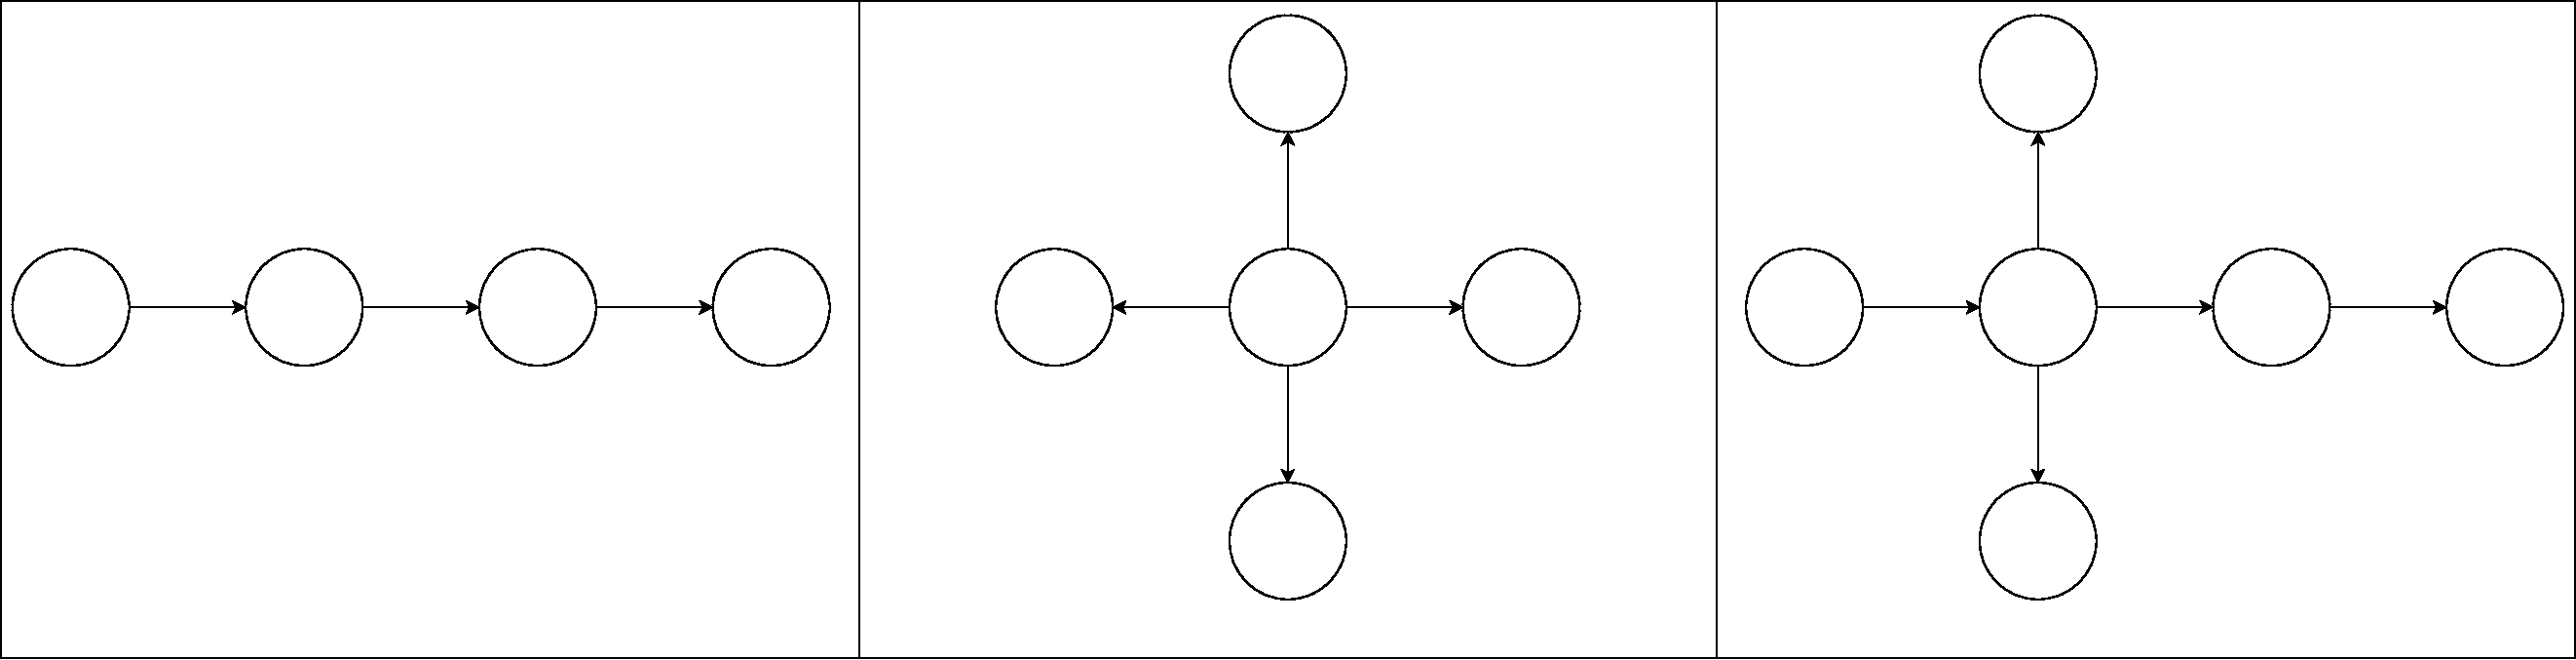
\includegraphics[scale=0.25]{c2/2-6-BGP-shape.pdf}
	\caption{Shape of basic graph pattern: chain, start, snowflake from left to right respectively.}
	\label{fig:2.6-bgp}
\end{figure}

SPARQL also supports other types of query apart from the SELECT query that was shown in the previous example. 
\begin{itemize}[noitemsep,nolistsep]
\item \textit{ASK} query to pose a ``yes/no" query and retrieve a binary ``true/fasle" in return.
\item \textit{CONSTRUCT} query to create new RDF graphs from a query return.
\item \textit{DESCRIBE} query to return details information of a resource.
\end{itemize}

Since the RDF data model allows heterogeneous data to be semantically described and linked, the SPARQL allows the data to be semantically extracted, integrated.
With the ability of expressing semantic search criteria, SPAQL could be the semantic query language for discovery heterogeneous things in the IoT~\citep{Richard:2013,Chun:2015}.
The newer version, SPARQL 1.1~\citep{Harris:2013} has included update and federation that is more adaptable to the dynamic and distributed environment of the IoT. 
C-SPARQL~\citep{Barbieri:2009} and CQELS~\citep{Le-Phuoc:2011} are the two query languages that extend SPARQL to enable evaluating linked stream data.


\section{Storing and Querying RDF data}
\label{s:sq}

In the previous section, we presented the overview of RDF data model and SPARQL.
This section provides an overview of how RDF data is stored and SPARQL query is executed. 
This topic is definitely important.
Understanding how RDF data is processed could help the later decisions on selecting data structures and algorithms.
Every data structures and algorithms have their own advantages and disadvantages in different situations.

\subsection{Physical organisation for RDF data}

The basic schema of RDF storage can be constructed simply.
For example, \cite{Harris:2005} represented RDF using relational model and SPARQL queries can be answered by translating to SQL queries.
The approach was demonstrated with 3Store that runs of MySQL, a relational database.
3Store uses a single table to store RDF graph and each triple is stored in a row. 
Each field in the triple table stores a hash value and the actual string values are stored in a symbol table, keyed on the hash value.
A constraint of this model is not only the translation of SPARQL queries to SQL queries, additional SQL queries might be required to determine the string representation from the returned hash values. 
3Store simplified the additional search constraint by joining the hash values back onto the triple table.

The approach of building RDF store using a back-end relational database was common in the Semantic Web community. 
Redland~\citep{Beckett:2001}, Sesame~\citep{Broekstra:2002}, Jena~\citep{Wilkinson:2003} and Virtuoso~\citep{Erling:2009} were the notable systems of this kind of RDF store.
This approach is quite simple and flexible, RDF graph can be stored in a generic fashion without a need of any customisation.
However, real relational DBMSs do not seem to be suitable to store RDF data in this fashion.
These systems rely on the optimisers of the back-end databases to optimise the queries.
This makes challenging for the databases to collect or produce relevant information for the optimisation.
The triple tables are exceptionally long and thin (little information per row). 
Useful amount of information requires a lot of rows to store.
Searching for a piece information becomes more difficulty since the number of rows increases.
Because, to return a query, the triple table has to be joined to itself and a query involves lots of joins rapidly becomes costly.

\cite{Abadi:2007} proposed to store RDF triples in different table called Property Tables.
Each table was assigned to a property and stored only the subject and object that are connected by the property. 
Despite the substantial advantages showed in the initial results of this proposal, a later evaluation showed that the performance improvement could be reduced if using different sort order  for the triple table approach~\citep{Schmidt:2008}.

RDF triples typically are stored in one or few long triple tables, iterating through the whole table to find one or some particular triples is impractical. 
Indexing can provide shortcuts to specific pieces information that a query requires. 
If indexes are available on one or several attributes, the search can jump straight to the triples that contain the search values.
The modern RDF stores create their own indexing strategy to index triples and overcome their large triple tables handicap.
Many stores, such as Hexastore~\citep{Weiss:2008} or RDF-3X~\citep{Neumann:2010}, do not need to store triples in table, because their indexes cover all possible access patterns.

The the idea of creating index for RDF graph is to allow efficiently retrieving the RDF triples that match a triple pattern. 
For example, the RDF triples that match the triple pattern (S P ?) can be retrieved on SPO index, in which S and P are keyed (S stands for subject, P for predicate and O for object).
The indexes are created materialising all possible of orders that cover all triple patterns.
Using three combinations of nodes in a cyclic ordering is enough to cover all query patterns (SPO, POS, OSP).
However, some RDF stores create less or more indexes depending on their query optimising or executing strategy.
Particularly, Hexstore and RDF-3X employ six index permutations, allowing them use merge joins that fastens the query executing.
Furthermore, the indexes contain all the data, so all the work can be done within them.

Selecting data structure to maintain these indexes is specially important for RDF storage.
Storing RDF triples in an optimal manner, such as multiple indexes, gives the accesses to matching triples more efficient.
Searching for the matched triples still slow if it requires to scan the whole index.
Data structure does not only influence the efficiency of searching but inserting, updating and the compactness of the storage.

There are variety of data structures, each of them is suitable for different tasks. 
Hash table or hash map are the data structures that are commonly used for memory-based storage~\citep{Date:1990}.
The part of the data that is as key search is hashed. 
A pointer to the location of the data in the database is stored at the memory position corresponding to the hashed value.
Hash data structure offers good performance as inserting and searching on hash table are $O(1)$ time complexity operations.
Popular RDF stores, such as Sesame~\citep{Wilkinson:2003}, SwiftOlwim~\citep{Ognyanoff:2007} and Jena~\citep{Seaborne:2010} used hash table to store RDF graph in memory.

However, some characteristics of hash data structure make it less desirable for disk-based RDF storage.
Of course, suitable hashing algorithm has to be utilised, otherwise, many hash collisions may occur.
In the point of view of SPARQL, to retrieve the set of triples that match a triple patterns, range searches are often utilised.
Meanwhile, hash does not provide physically ordered data based on its logical order, for example sorted order. 
That means it does not guarantee if two entities that are similar to each other are stored next to each other.
Triples that match a triple pattern are not guarantee to be stored in a same disk block or a sequence disk blocks.
Disk seek would be required for retrieving every single triple, creating massive searching and reading.

B-tree data structures, in particularly the B$^+$-tree variants, are the most common data structure for implementing disk-based indexes~\citep{Comer:1979}.
B-tree data structures are self-balance tree structures.
Each node in a B-tree has a number of child nodes.
The height of a tree is proportionate to log$_{n}$ where n is the fanout - the number of child nodes that a node can have.
The size of the fanout defines the height of a tree, and the height of the tree equals to number disk seeks required to search a data item. 
The height of the tree can be reduced by increasing the size of the fanout.
Consequently, the number of comparisons required to determine the child nodes to access increases when the fanout gets larger.
B-tree data structure is useful for hard disks because they can make a good use of such block-based memory medium's characteristics by keeping the tree nodes sized to a block.
A disk block (typically around 4kB-8kB) is quite large, hence, the height of the tree is often low, of course, few disk seeks are required. 
Retrieving a block costs equally to retrieve partial block.

B$^{+}$-tree is a variant of B-tree that modifies B-Tree.
B$^{+}$-tree allows all pointers to actual data to be stored in the leaf nodes, and leaf nodes are linked to allow sequential traversal over them.
Comparing to hash data structure, B-tree offers much better performance for range search~\citep{Ullman:2001}.
Therefore, B$^{+}$-tree has been attracted to creating indexes for RDF data.
The relational databases that have been used as back-end database for RDF triple store made exclusive of this data structure. 
The other systems, such as Jena TDB~\citep{Owens:2008} or RDF-3X~\citep{Neumann:2010}, were implemented with their own versions of B$^{+}$-tree.

The approaches seem to be attractive to store RDF data for cloud-based system or IoT nodes that are powerful workstation.
Processing RDF data on the edge nodes would be more challenging.
The environment on the edge IoT is more dynamic, hence updating ability is more important.
Using memory-based RDF storage using hash table could be a suitable solution as inserting with hash table is O(1) time complexity operation.
However, IoT edge nodes often have limited memory, memory-based storage would not scale on edge nodes. 
Disk-based storage would enable more data can be stored on edge nodes.
However, edge nodes are often equipped with flash-based storage.
B-tree data structure is not well-suited with the characteristics of this type memory medium.


\subsection{SPARQL Processing}

A SPARQL query is often processed in the followings sequential step:
\begin{enumerate}[noitemsep,nolistsep,label=(\roman*)]
\item Compile SPARQL query to an internal form and convert it to canonical form;
\item Choose the candidate physical operators;
\item Generate the query plans and choose the cheapest on to execute. 
\end{enumerate}

The first step transforms the query string to an internal format that is easier to process further. 
In this step, some minor optimisations can be utilised such as removing irrelevant triple patterns.
The second step is to produce low-level operations for processing the query for example, index scanning or joining.
The operations are selected associatively with the information, such as data structure on disk, availability of indexes or statistic of data, to speed up the query. 
In this step, the cost of executing of each operation is calculated and is assigned to them.
In the final step, a set of potential query plans are created from the operations produced from the previous step. 
In a query plan, the operations and the order in which the operations are performed influence the performance of a query.
Choosing the best query plan is also performed in this step. 
A cost model is assigned to compute cost for each query plan.
The cost model is often based on the selected operations and the order in which the operations will be performed.
The cheapest query plan will be chosen and executed.

Answering a SPARQL query requires multiple joins of RDF triples that match the triple patterns.
This leads join operation to be the most-used while executing SPARQL queries. 
Different join algorithms are differentiated by how the input data is organised and require different amount of computing resource to perform.
Indexed nested loop, hash join and sort/merge join are the join algorithms that are useful for joining RDF data~\citep{Owens:2011}.

The index nested loop join~\citep{DeWitt:1993}(INLJ) uses nested loop to for joining two sets. 
For each item in one set (called the outer input), it scans the entire the other set(called the inner input) and finds compatible items.
The performance of INLJ relies on the availability of index on the inputs.
This algorithm is faster than the brute force algorithms which often have O(n$^{2}$) time complexity with n is the size of the data being examined.
If index is available on the inner input and there is no match, only few operations need to be utilised in stead of scanning entire inner set.
This algorithm is especially effective in terms of reducing computation in the situation that:
the outer input is small and the inner input is very large.
INLJ is useful for utilising join over RDF data since RDF stores are often designed with comprehensive indexing strategies~\citep{Owens:2011}.

Hash join is the algorithm for joining two set based on hash function~\citep{Ullman:2001}. 
It performs two single scans over the inputs.
The first scan is to create hash table for the first input.
The hash table contains hashed value of join attributes of each item and a corresponding pointer to the item. 
The compatible items on the second input are found by scanning and looking back to hash table.
This algorithm does not require indexing on inputs and scales in a linear manner with the size of the inputs.

Merge join algorithm requires the items in two input set are sorted on the join attributes~\citep{Ullman:2001}.
Therefore, the join can be execute by simply scanning of both inputs and comparing on the join attributes to produce join results. 
Sort/Merge join simply sorts the inputs as required and performs merging.
Merge join is always faster than hash join or nested loop join if data is sorted correctly.
However, in case the inputs have to be sorted, the performance of this algorithm largely relies on the performance of the sorts.

Selecting the right algorithms for implementing the join operations of query processors is obviously important.
Especially, many join operations may be required to execute SPARQL query, and they contribute the most on time consumption and resource consumption of SPARQL processing. 
The INLJ join requires very little memory and also is efficiently for paralleling~\citep{Sheu:1991}.
However, in disk-based stores, INLJ might require higher number of disk seeks comparing to hash join or sort/merge joins.
Hash join does not require searching or sorting as data can be scanned sequentially on disk, but memory is required to hold the the intermediated results.
It is less tractable if no memory is available.
Merge join is fastest algorithm if sorting is not required. 
For this reason, RDF engines such as, RDF-3X~\citep{Neumann:2010}, often try to use merge join as possible. 
RDF-3X orders the join operations accordingly to the sort order of data in the working set.

Selecting the right joins is more challenging to execute SPARQL on IoT edge nodes.
The former query planners and query optimisations select the joins and order the joins with out taking resource consumption(memory consumption) into account. 
Of course, in unlimited capabilities storage and processing power environments such as cloud infrastructure, minimising the time spend on the join is the highest priority. 
On the edge nodes, resource consumption of the joins must be considered as inappropriate resource usage may result system failure.

\section{Summary}

In this chapter, the relevant concepts in the IoT, the Semantic Web and the fundamental RDF data processing was introduced as the research background of the thesis.
Section~\ref{s:iot} introduces three visions of the IoT: Thing-oriented vision, Internet-oriented vision and Semantic-oriented vision.
This section also highlights the need of the semantic technologies in solving the interoperability problems and the emergence of the edge computing for the IoT. 
In section~\ref{s:sw}, the suite of Semantic Web technologies including RDF data model, inference, SPARQL query language are introduced.
RDF data model is a graph-based data model which allows a flexible way to describe things properties, things relations and link different things together.
The inference ability allows RDF data to be reasoned to derive new concepts, new relations from a base dataset, therefore, allowing the meaning of data to be shared.
To query RDF data, SPARQL query language was designed as graph-matching query language.
SPARQL allows the data to be semantically extracted, integrated.
How RDF data is stored and SPARQL query is executed is presented in Section~\ref{s:sq}.
Indexing is critical important for the RDF data to be stored to allow efficient querying.
Storing RDF in-memory will allow fast inserting and querying, however, memory on the edge nodes is usually not enough to hold all the data in the memory. 
B-tree is most common data structure to implement indexes for RDF data in disk-based RDF storage.
However, B-tree may not suitable for flash-based storage and this issue will be more precisely presented in the next chapter.
Answering SPARQL query requires many join operations to be utilised.
Different algorithms for implementing joins result different time consumption and resource consumption of joins.
Executing SPARQL query on IoT edge nodes requires the query planners and optimisers take resource consumption into account.
}









 
%\chapter{Internet of Things: Semantics}
\lhead{Chapter 3. Internet of Things: Semantics}

\section{Justification for a semantic IoT}

\subsection{Importance of the Semantic Technology for the IoT}
\label{ss:stiot}

As mentioned above, the IoT would destine with huge number of interconnected objects.
Recently, there have been around 7 billions active IoT devices and this number is still growing with an upper trend~\footnote{https://iot-analytics.com/state-of-the-iot-update-q1-q2-2018-number-of-iot-devices-now-7b/}.
Searching for a device or for a piece of information among billions IoT devices and terabytes of information would become exponentially harder.
Enabling the integrating of the information from billion sources would become more challenging.
Big data solutions~\citep{Chen:2014} and cloud platforms~\citep{Botta:2016} could provide mechanisms to handle huge amount of information.
However, efficient methods that could structure, annotate, link and make sense of the information would still be needed~\citep{Barnaghi:2012}.
Regarding the challenge of how to organise and interconnect IoT information, the Semantic Web technology offers \textit{Resource Description Framework(RDF)}~\citep{Lassila:1999}.
RDF allows flexible way to describe data and its properties, relations and allows data to be linked.
Therefore, ``Things" can be searched and grouped with common properties~\citep{Chun:2015} and more related ``Things" can be discoverable~\citep{Serena:2017}.

As billions of IoT devices will be interconnected to create the IoT, and they must be able to operate and communicate with each other autonomously.
Therefore, enabling the interoperability among IoT devices has been considered as one of the most fundamental requirements for a smart IoT.
Recently, more than 300 IoT platforms have been developed and they were still fragmented due to the lack of the interoperability.
\cite{Manyika:2015} has estimated that the potential economic benefits of the IoT might be reduced by 40 percent due the missing interoperability.

The interoperability challenges in the IoT can be divided into \textit{connectivity level} and \textit{semantic level}~\citep{Kiljander:2014}.
The issue of interoperability in the connectivity level refers to how to allow IoT devices to transfer data with each other.
Whereas, in the semantic level, the problem refer to how different IoT devices, platforms are enabled to exchange data with unambiguous and shared meaning.

At the connectivity level, the interoperability could be provided by creating mechanism to deal with the heterogeneity of communication technologies(WiFi, ZigBee, ANT+), network protocols(CoAP, MQTT, XMPP). 
The proposed solutions suggested that IoT platforms would offer a pool of standardised communication protocol, hence, device 
manufacturers would be able to select the appropriate communication protocols~\citep{Noura:2017}.
The IoT gateway~\citep{Zhu:2010} seems to have been an attractive solution for such mechanism in an IoT platform~\citep{DaXu:2014}.
Network protocols can be selected or translated via gateway devices that enabling the interoperability in this level~\citep{Bandyopadhyay:2013}. 

However, interoperability in the connectivity level can not fulfil the interoperability required in the IoT~\citep{Kiljander:2014}.
Applications, systems can not make use of the data from different IoT platforms without understanding it. 
In the semantic interoperability level, the focus lies on the mechanism that allows the meaning of data and services to be shareable.
Using the semantic annotation can provide IoT data, services with machine-understandable descriptions on what the data represents or what the services offer~\citep{IERC:2013}.
Therefore, IoT data and services can be exchanged among IoT devices and crossing IoT platforms. 

The Semantic Web technology has been the preferable solution for the semantic annotation on the Web and could utilise also in the IoT~\citep{Jara:2014,Noura:2017}. 
RDF data model has been a suitable data model for semantic annotation~\citep{Oren:2014} and also ideally for providing semantic annotated for IoT data~\citep{Wei:2009}.
The extensions of the RDF are the RDF Schema(RDFS), Ontology Web Language(OWL) that define the structure for the RDF.
The RDFS and OWL increase the expressiveness of RDF data by defining domain and range for properties, as well as, its hierarchy such as sub-class, sub-property.
Therefore, IoT data could be represented in different abstraction levels and its semantic could be enriched depending on requirement~\citep{IERC:2013}.
Based on RDF, RDFS and OWL, different ontologies could be developed for information reusability and shareability thus enabling the semantic interoperability. 

Moreover, the collected data from IoT could create situation awareness that enable smarter application, systems~\citep{Barnaghi:2012}.
These smart applications, systems have been well-known as context-awareness systems~\citep{Baldauf:2007}.
They could react adaptively to the change of their context. 
The context-aware systems require logical reasoning processing to derive the context from the data.
The semantic representation formalism used in the Semantic Web provide logical reasoning to derive context, to infer new context from existing knowledge and rules.
The OWL as ontology-based frameworks for context modelling and reasoning have been used in pervasive computing domain~\citep{Mikko:2009,Bettini:2010}, and now in the IoT domain~\citep{Perera:2014}.


\section{Challenges for a Semantic IoT}

\section{Semantic Technologies for the IoT}

\section{Challenges to implementing an edge-based semantic architecture}


%==================================================================================================
\section{Hardware characteristics of IoT Edge Devices}
%==================================================================================================

Recent advances in the technologies of embedded processor have increased the processing capabilities of IoT edge devices.
Based on the computational capability, IoT devices can be categorised into two categories: low-end devices and high-end devices.
The low-end IoT devices which are very constrained in terms of resources including energy, CPU(less than 100MHz) and memory capacity (less than 100 kB).
Popular examples of devices in such category include 
Arduino~\footnote{https://www.arduino.cc/}, 
Zolertia~\footnote{https://zolertia.io/}, 
OpenMote node~\footnote{http://www.openmote.com/}, etc.
The second category consist in high-end IoT devices, which includes single-board computer such as Raspberry Pi~\footnote{https://www.raspberrypi.org/}, 
Beagle Bone board~\footnote{https://beagleboard.org/bone} or 
smartphones.
The high-end devices are more powerful than the low-end devices.
They have enough resources and adequate characteristic to run software based on tradition operating systems such Linux or BSD. 

The current trend seems to be that all the devices communicate directly with the cloud and interact with each other through web services~\citep{E.A.Lee:2014}. 
Several significant problems with traditional cloud of things~\citep{Parwekar:2011} have been revealed, for example, the issues with scalability, latency, bandwidth. 
These problems are not new to typical web applications, they are exacerbated in the IoT space because of the fundamental differences between IoT and web services~\citep{Zhang:2015}.
To deal with the issues, the task of processing the the task of processing the data is pushed to the edge devices, introducing concepts of Fog computing~\citep{Bonomi:2012}, Edge Computing~\citep{Salman:2015}.
Due to the limited computational capabilities of low-end devices, they are often deployed in the lowest layer of the IoT that perceive the real-world data.
On the on the hand, the devices in the high-end category contain suitable hardware for performing such operations~\citep{Kruger:2014, Morabito:2017}.

IoT gateways, in the centralised scenarios, are the devices that are used to settle the heterogeneity between different networks and the Internet~\citep{Zhu:2010, Petrolo:2017}.
A separate gateway service has to be provided for each type of IoT device that is deployed~\citep{Zachariah:2015}.
Essentially, today's IoT gateways present problems with the distributed scenarios, to enable communication between IoT devices networking interoperability alone is not enough.
More functionalities, for example interoperability at data annotation level, are requires on the gateway level~\citep{Desai:2015}.
The gateway may have to execute some data processing functions, such as data aggregation.
Such high-end devices are lightweight and have computation resources that are feasible to be implemented as the smart IoT gateway.

As presented in the previous chapter, the Semantic Web is a promising key technologies that enable the semantic interoperability for the IoT.
RDF engines have been proposed as semantic integration gateways for IoT data~\citep{Kiljander:2014}.
Having an RDF engine on such devices will enhance the build for the smart IoT gateway.
Placing computational nodes closer to source devices offers opportunities to improve performance and to reduce network overhead, but also flexibility for the continuous integration of new IoT devices and data sources. 

In order to understand how to create an RDF engine on that type of devices, it is obviously important to understand how the hardware on which the engine is to be run behaves.
This section offers a brief overview of the components of the high-end edge devices that are particularly relevant to DBSMs performance, with a focus on the commonly used o ARM architecture and flash-based storage.

%Memory hierarchy CPU Register $\to$ L1 Cache $\to$ L2 Cache $\to$ Memory $\to$ Flash Storage.
%, with a focus on the commonly used o ARM architecture and flash-based storage.

%==================================================================================================
\subsection{CPU}
\label{ss:CPU}
%==================================================================================================

The IoT edge devices are mostly equipped with ARM(\textit{Advance RISC Machine}) processors which is an 32-bit \textit{reduced instruction set computing (RISC)} architecture for computer processors.
ARM processors possess a unique characteristics that are desirable for lightweight, portable, battery-powered devices.
First, processors that have a RISC architecture typical require fewer transistors than those of general-purpose processors, leaving plenty of space on the chip for application-specific macro-cells.
Second, ARM instruction set architecture and pipeline are designed to minimise the uses of energy consumption.
Third, ARM is highly modular, the mandatory of an ARM processor is the integer pipeline, all other components are optional, which gives a lot of flexibility in building application-specific ARM-based processors.

Among various ARM processor families, ARM Cortex-A series~\footnote{https://www.arm.com/products/processors/cortex-a} are mainly developed for open operating systems and applications including single-board computers, home gateways. 
Beside integer pipeline, Cortex-A series is included superscalar and caches to improve the performance of the chip~\citep{Wang:2011}. 

Pipelining is the process of dividing incoming instructions into its component parts and executing them sequentially~\citep{Molnar:1994}.
The pipelining allows faster CPU throughput, one stage 1 of the pipeline has finished executing part 1 of instruction 1, it is able immediately begins executing part 1 of instruction 2.
The RISC instructions are simpler than those used in ~\textit{complex instruction set computer (CICS)} processor.
While CICS instructions varied in length, RISC instructions are all the same length and they are more conducive to pipelining.
Ideally, each of the stages in a RISC processor pipeline should take 1 clock cycle, so that, if the pipeline is kept full, the processor takes an average of one clock cycle to finish an instruction.
Pipeline length is vary between ARM processor design: the ARM Cortex A7~\footnote{https://developer.arm.com/products/processors/cortex-a/cortex-a7} has a pipeline length of 8 stages, as opposed to 13 for the ARM Cortex A8~\footnote{https://www.arm.com/products/processors/cortex-m/cortex-a8.php}.

Superscalar architecture~\citep{Smith:1995} was applied in ARM Cortex A8 processor and later versions of ARM Cortex-A series~\citep{Wang:2011}.
Superscalar implements a form of parallelism called instruction-level parallelism within a single processor.
That enables processor to fetch and complete more than one instruction simultaneously if the instructions are independent.

Pipelining and superscalar techniques increase CPU throughput without the requirement of increasing clock frequency.
Both require data-independent instructions to operate with full effectiveness.
If one instruction depends on the output of another, it cannot enter the pipeline until the first instruction has completed.
Fortunately, modern versions of ARM Cortex A series have ability to process instructions out of order, allowing instructions that do not depend in the pipeline to jump the queue.
Out-of-order execution is usually highly effective, except in the situations that operations are repeatedly executed on a small number of pieces of data.
Such situation results in a lot of dependencies within the instruction stream~\citep{Zukowski:2006}.

ARM Cortex-A series have Level 1 (L1) and Level 2 (L2) caches~\citep{Wang:2011}. 
When the CPU is looking for information in memory, it will check its caches first before searching and transferring data from main memory.
If one the caches has the information, the CPU can access it with cache latency which is much smaller than main memory latency.
The cache line in ARM Cortex-A series is typically 32 bits.
The L1 cache consist of two parts, each for data and instructions. It is small (16-32 Kb for each part) and extremely fast. 
Data can usually be retrieved from this level in from 3 to 4 clock cycles. 
The L2 cache is larger and be up to 1-4 MB, and somewhat slower, requiring around 14-21 cycles to access. 
However, this is still an order of magnitude faster than main memory~\citep{Drepper:2007}.

As long as data and instruction flow is sufficiently predictable, information can be held in and retrieved from cache, the throughput of RISC processors is able to utilise with full effect. 
Given above information, it can be seen that the applications which run on ARM-based can achieve high performance if ensuring that data is compact and is located contiguously where possible, maximising cache utilisation.
DBMSs have historically performed poorly at this task~\citep{Ailamaki:1999}.

%http://processors.wiki.ti.com/index.php/LMBench_on_ARM_Microprocessors
%http://ithare.com/infographics-operation-costs-in-cpu-clock-cycles/
%==================================================================================================
\subsection{Memory}
%==================================================================================================

The amount of Random Access Memory(RAM) on high-end IoT edge devices are much higher than that of low-end IoT edge devices.
Single board computers can have from 256MB to 2GB of RAM.

Storing data in RAM is relatively simple matter.
RAM has a constant access time and its performance is vastly better than that of secondary memories, particularly flash-based storage of IoT edge devices. 
The throughput of RAM is high, this seems the requirement for pieces of logically contiguous data to be placed next to each other is looser.
However, the latency to access data from RAM can be in excess of 200 nanosecond~\footnote{https://www.7-cpu.com/cpu/Cortex-A8.html}.
This makes it impractical for the processors to wait for memory every time they need access to a piece of data~\citep{Drepper:2007}.
Data going to and from RAM is held in caches on the processor, as these had been previously explored in more depth in Section~\ref{ss:CPU}.
In practice, the contiguity of data access remains important even when working with a main-memory system.

The difficulties in working with RAM are that it is limited in size and not persistent.
Although the capacity of RAM that is available on high-end devices increases, it still limited to for an in-memory DBMSs on such type of machines.
Data should be mainly organise on next level of the next layer of memory hierarchy, the persistent storage layer.

%https://www.7-cpu.com/cpu/Cortex-A8.html
%==================================================================================================
\subsection{Flash-based storage}
\label{ss:flash}
%==================================================================================================

The majority of single board computer make use of flash-based storage such as SD cards or eMMC cards. 
Compared to disk-based storage, flash memory has attractive features such as lighter and smaller, better shock resistance, lower power consumption, faster access time and no mechanical seek and rotation latency~\citep{Koltsidas:2011}

Flash memory is a type of electronic memory that stores information in arrays of memory cells~\citep{Kono:2018}. 
Flash cells are available in two varieties, \textit{Single Level Cells (SLC)}(SLC) and \textit{Multiple Level Cells (MLC)}, that stores one, two or three bits per cell perspectively. 
As MLC devices is more dense that SLC one while both writing and reading to a multiple level cell takes longer than a single level one.
For these reasons, SLC devices are mainly used for high performance purposes, while MLC ones typically applied where large capacity is required. 
Depending on how flash cells are connected to form arrays, flash memory is classified into NOR flash and NAND flash.
Since only MLC flash cells and NAND flash memory are suitable for storage devices, they are widely used in building flash storage. 

In flash storage, arrays of flash cells are organised into pages and pages are grouped into blocks~\citep{Kono:2018}. 
In most of storages, the size of a page is typically 2kB or 4kB and a block typically contains 64 pages.
There are three operations on flash memory: read, write, and erase. 
A page is the smallest unit that is can be read from or written to flash memory.
An empty page has all its bit set and writing a page implies turning some of the bits to 0. 
Resetting some bits in a page is not possible, rather, the whole page has to be reset before it can be set again.
Resetting all the bits of a page is referred to as erasing and can not be done in page basic. 
A block is the smallest structure of flash storage that can be erased. 
Consequently, after erasing a block, each one of its pages can be written to only once. 
In order to overwrite a page, the whole block needs of be erased first~\citep{Kono:2018}. 
Erasure takes much longer time than read/write and the need of the erasure is well-known as the erase-before-write limitation of flash memory that incurs several penalty on flash storage performance.
For instance, the write-in-place operation, that updates a single piece of data in a block, is inefficient as it consists of two operations on the entire block: erase and write.
An other important limitation of flash memory is that, in its lifetime each flash block is only capable of a finite number erasure. 
After that, the flash block becomes unusable. This limitation is referred to as memory wearing~\citep{Kono:2018}.

The I/O behaviours of flash storage are particularly relevant for RDF stores, which are generally required to process a great many very small data point. 
This is particularly relevant for RDF stores, which are generally required to process a great many very small data points.
An extensive study on the performance of flash storage~\citep{Ajwani:2008} found that flash-memory yields better random read performance than magnetic disks, but a much worse random write one.  
Without mechanical seek, data location is not as important as it is on disk-based storage.
In this situation, assuming the processing cannot be kept fully sequential, writing time is extremely important because the write-in-place operation is not supported. 
Specifically, the erase-before-write limitation degrades the efficiency of disk-based data structures~\citep{Bouganim:2009} and caching mechanisms~\citep{Graefe:2007}. 
Due to the flash I/O behaviours, the commonly used indexing structure in RDF triple store (presented in Section~\ref{s:rdf_data_management}) is not optimal for writing on flash storage.

%==================================================================================================
\section{Database Management Techniques for IoT Edge Devices}
%==================================================================================================

From characteristics : $\to$ indexing techniques for flash memory and $\to$ memory adaptive 

%==================================================================================================
\subsection{Flash-awareness Data Structure for Storage}
%==================================================================================================

%==================================================================================================
\subsubsection{Flash-awareness indexing}
%==================================================================================================

As discussed in Section~\ref{ss:flash}, flash storages have erase-before-write limitation that makes random writes inefficient.
A great deal of research has focused on increasing the throughput of flash storage when writing small chunk in a random fashion.
On hardware layer, flash storage controllers try to minimise the effect of erase-before-write limitation on random write by employing a software layer called \textit{Flash Transaction Layer(FTL)}~\citep{intel:1998}.
The main purpose of the FTL is to provide logical-to-physical address mapping of file system and flash memory perspectively.
Different types of flash storage may employ different FTL algorithms~\citep{Chung:2009}.
From database management system perspective, the FTL is a black box.

FTL algorithms are primarily designed with file systems in mind and are not well-suited for database workloads~\citep{Lee:2007}.
Random write operations in file systems are mostly required for metadata. 
When executing typical database workloads, random write operations may be performed over the whole disk address space. 
As an aim that improves write efficiency for flash-based databases, the \textit{in-page logging(IPL)} scheme is proposed~\citep{Lee:2007}.
Changes of a data page are not written directly to disk but to log records that is associated with the page.
Data and its logs are co-located within the same physical block of flash memory, i.e, in the same erase unit.

The main principle of the design of flash memory access methods is avoiding in-place updates and random writes.
\cite{Nath:2008} approached this principle by avoiding \textit{sub-block deletions} and employing \textit{semi-random writes}.
Sub-block deletion that deletes a portion of data in a block, on flash memory, would requires the undeleted data in the same block to be first migrated to a new block.
Therefore, sub-block deletions can be two orders of magnitude more time than block deletions.
Instead, access methods should employ semi-random writes, according to which individual pages within a block are written sequentially from the start of the block; the write pattern can select blocks in any order.
The experimental evaluation of this principle was found to yield performance similar to the one of sequential writes.

B-tree index is a data structure that is widely used in many file systems and database management systems for disk-based storage~\citep{Ullman:2001}. 
However, the frequent random writes of B-tree may degrade the efficiency of B-tree index on flash memory.
There have been an extensive research in order to optimise B-trees for flash memory.
The proposed approaches can be grouped into: buffer-based approach, structure-modified approach or hybrid approach~\citep{Ho:2016}.

The first group have used extra memory resource as write buffer to improve the performance of FLT. 
\textit{BFTL} was proposed as a software layer on top of FLT that allows B-tree to work on flash memory with the same fashion as on magnetic disk~\citep{Wu:2007}.
To overcome the erase-before-write limitation, BFLT propose storing tree nodes as a sequence of log records spread over multiple flash blocks.
BFTL consists of two components: a reservation buffer and a node translation table.
The modifications are temporarily stores in the reservation buffer, the the buffer is full they are flushed to flash memory.
BFTL reduces the number of write operations, but reading node data that is scattered on different pages can become expensive.
BFTL consumes also additional memory to persist the node translation layer. 
To solve the problem of scattered node data, IBSF is buffer management scheme that stores all index units associated to one node within one page~\citep{Lee:2010}.
IBSF efficiently eliminates redundant index units in the buffer to delay the time that the buffer is full.
However, storing each B-tree node in one page results in pages can be used up quickly, thus garbage collection will occur frequently.
\textit{Lazy Adaptive Tree (LA-tree)} was another approach that uses external buffer to delay the write on flash memory.
LA-tree adds a buffer to the nodes at every level of the tree starting from the root~\citep{Agrawal:2009}.
The updates on a node and its descendants are cached within the respective buffers. 
The inserts is first cached in a root buffer, if the root is full they are pushed in a batch to the buffers at lower levels.

On the other hand, the other approaches have modified the structure of the B-tree adaptively.
Unlike the buffer-based approaches for tree index on flash storage, others approaches aimed to modified the structure of B-tree instead of using extra memory buffer.
\textit{Wandering tree}, which was proposed for flash file system \textit{JFFS3}~\citep{Bityuckiy:2005}, stores the updates in free pages, therefore, it does not have to erase a page before writing.
However, Wandering tree can lead to increased number of write operations when the height increases.
{\Large $\mu$}-tree overcomes the limitation of Wandering tree by storing all the updated nodes along the path from the top to the bottom onto a single flash memory page~\citep{Kang:2007}.
{\Large $\mu$}-tree allows the size of each node to vary depending on the level within a tree and the its height.
However, $\mu$-tree doubles the number of pages to store the same data as a B-tree and its page-layout is space inefficient.
{\Large $\mu$}*-tree was an enhanced version of $\mu$-tree that allows the node size at each level to be flexible and each page to have its own layout~\citep{Jin-Soo:2013}. 
{\Large $\mu$}*-tree attempts to postpone its height growth by shrinking the size of leaf nodes. 
Similarly to $\mu$-tree, $\mu$*-tree consumes much more pages comparing to a B-tree, nodes are often splinted, and the height of a tree can increase rapidly as nodes are smaller than in a B-tree. 
FD-tree was another variant that modifies B-tree adaptively for flash memory~\citep{Li:2010}.
FD-tree aims to reduce the number of random writes with the logarithmic method and fractional cascading techniques.
On top of FD-tree is a small B$^{+}$-tree that fit in main memory and few levels of sorted runs are added at the bottom. 
New elements are first added to the head tree and moved to lower levels when the head tree is full.
Each node at lower in the FD-tree can be either a typical index node or a fence node, i.e., a pointer to a page in a lower level.
The changes are merged to the lower level sorted runs in batches.
The experimental evaluation of this technique shows that it outperforms all other B$^{+}$-tree variants at both search and update-intensive workloads.

The hybrid approaches are the approaches that combine of buffer-based approach and structure-modified approach.
MB-tree keeps a \textit{batch process buffer (BPB)} in the main memory and \textit{leaf node headers(LNH)} on the flash storage for meta-data about nodes~\citep{Roh:2009}. 
An leaf node header occupies a single flash page.
When the buffer is full it chooses the node that has the most modifications and moves it to the physical layer hence, it groups multiple data modifications in one write. 
The MB-tree achieves an efficient trade-off between the page-write count and search time through a reduced write count by the BPB as well as enhanced search time by the LNH. 
In order to take advantage of the parallelism and sequential write of the flash memory, the author of MB-tree also proposed \textit{Always Sequential B-tree structure (AS B-tree)}~\citep{Roh:2014}.
AS B-tree also buffers write operations before pushing them to flash storage.
However, when the data is moved it is placed at the end of a file instead of overwriting what allows them to avoid in-place writes. 

The arrival of flash storage was also attracted to the researches on optimising hash index for such storage medium.
MicroHash an efficient external memory index structure for Wireless Sensor Devices (WSDs), which stores data on flash by time or value~\citep{Zeinalipour:2005}. 
However, the MicroHash can only be applied for wireless sensor which manipulates data directly to raw NAND flash.
MLDH proposed a multi-layered hash index scheme, in which the capacity of each level is twice as its upper level~\citep{Yang:2009}. 
Updates to the MLDH is first cached in an in-memory buffer, and the buffer is merged with hash indexes on flash when it is full.
\cite{Wang:2010} proposed a flash based self-adaptive extendible hash index.
Similarly to IPL storage model, a hash bucket consists of both data region and log region.
Each hash bucket occupies a block (erase unit) of flash. 
Update and delete operations are perform in the log region, so in-place updates to the data region can be delayed.
In addition, a Split-or-Merge (SM) factor, which is dynamically adjusted according to the log/data ratio, is added to make the index self-adaptive.
Hybrid Hash Index~\citep{Yoo:2012} delays split operations which cause additional writes and erase operations by using overflow buckets.
If the number of overflow buckets attached to a bucket has reached the ceiling, the Hybrid Hash Index determines whether a split operation is triggered according to the ratio of update and delete records in that bucket.
Another Lazy-Split scheme that avoids removing object in place was proposed in~\citep{Li:2008}. 
Two variations of a linear hashing index were presented in the Lazy-Split scheme. 
The first variation is similar to the standard linear hash index that is suitable for search-intensive workloads.
The second variation is more suitable for update-intensive workloads.
Hash buckets are split lazily in batches to reduce the cost of writes, of course, of some additional cost when searching the index.

%==================================================================================================
\subsubsection{Flash-aware Buffer management}
%==================================================================================================

Researchers also has considered novel buffer management scheme over flash storage.
For the cases, data is stored persistently on flash storage and subset of persistent data are cached in main memory.
The tradition caching schemes for magnetic disk, such as \textit{Least Recent Used LRU}, are not efficient for flash storage due to the asymmetric I/O of flash memory~\citep{Graefe:2007}.

\textit{Clean First LRU (CFLRU)} was proposed as an alternative LRU scheme for the on-disk buffer cache of flash storage~\citep{Park:2006}.
CFLRU aims to exploit the asymmetric performance of read and write operations of flash storage.
It priorities a clean page to be a victim rather than dirty pages because writing cost is much more expensive.
With this strategy, CFLRU was able to reduce the average replacement cost by 26$\%$ compared to the LRU algorithms.
This is irrelevant when only write requests are involved. 
Thus, it is not useful for enhancing random write performance.

\textit{Block Padding LRU (BPLRU)} was the scheme that aimed for write-intensive database applications on flash storage~\citep{Kim:2008}.
This scheme groups main memory buffers in blocks that are equal in size to the flash erase-unit. 
Pages is replaced with erase-unit granularity following LRU policy.
If not all pages in a dirty block are in the main memory, the absent pages are read from storage and the whole block is written to new flash location without the need for erasing.
Additionally, a block that was written sequentially is moved to the tail of the LRU queue and becomes the next victim.

\textit{Clean-First Dirty-Clustered (CFDC)} aimed to enhance the write performance of CFLRU by flushing pages in clustered fashion~\cite{Ou:2009}.
CFDC minimises the number of writes and exploits the spatial locality of victim pages.
Dirty pages whose page numbers are close to each other, and therefore are likely to be physically stored near one another, are clustered together in page clusters.
The authors of CFDC later proposed a model for adjusting the size of the buffers for clean pages/dirty pages according to the storage device's read/write ratio~\citep{Ou:2010}.
Thus, write operations become more flash-friendly.

\textit{Cold Clean First LRU (CCF-LRU)} improves the performance of CFLRU in a different way~\citep{Z.Li:2009}.
It tried to reduce the number of write accesses by keeping track of the condition (clean/dirty) and status (hot/cold) of pages.
CCF-LRU uses two LRU queues to store data pages in main memory.
The first queue keeps cold$\&$clean pages while hot$\&$clean pages and dirty pages are kept in the other queue.
When the cache is full, data from the cold $\&$ clean part will be released from main memory to storage first.
If the cold$\&$clean is empty, then data from the mixed queue is released.
This scheme does not only delay the write operations for dirty pages but also delays the eviction of frequently accessed clean pages, that can increase the cache-hit ratio. 
However, it can not detect the hot clean pages as it has no techniques to control the size of the cold$\&$clean part.
This part is likely to be empty and newly read page is evicted immediately.

The limitation of CCF-LRU was improved in \textit{Adaptive Double LRU (AD-LRU)}~\citep{Jin:2012}.
In AD-LRU, two queues are also used to capture the frequency and recency of data pages.
The authors introduced a parameter to set the lowest limit for the size of the code queue.
The size of two queues can be adaptively resized to be suitable for different access patterns such as random, read-most or write-most.

\textit{Flash-based Operation-aware buffer Replacement (FOR)} approaches the problem from a different perspective~\citep{Lv:2011}.
The victim page is indicated by combining between the future operations and the page state 
The benefit of keeping a page in main memory is quantified by distinguishing the page state (clean or dirty) and its next operation(read or write).
In consequence, they introduced \textit{inter-operation distance(IOD)} and \textit{operation recency} for page operation to quantify its frequency and recency, receptively .
However, fore every accessed page, two data points for the last read and last write have to be saved, and every operation has to be recorded.
Hence, list that used to store these data is possibly very long.
To overcome these issue, FOR$^{+}$ was introduced that tries to approximate the IOD based on the currently cached pages.
The approximation adopts the metrics of the weight with binary representations to approximate the combination of operation type and page state.
Both FOR/FOR$^{+}$ are built on an LRU basis there may be scan resistance issues. 
Furthermore, both FOR and FOR$^{+}$ need carefully chosen cost estimation for reads and writes and FOR$^{+}$ needs another tuning parameter for the size of its cold page index.

\cite{Anwar:2017} considered the overhead of garbage-collection can degrade the performance of the FTL of flash storage devices.
They took garbage collection cost into account when introducing \textit{Log-buffer aware cache replacement policy (LAB)}.
LBA attempts to streamline the write operations to flash memory, resulting in a low overhead to the FTL upon performing garbage collection.
The life span of flash memory is also increased as the number of merge operations of the FTL was reduced.

%==================================================================================================
%\subsection{Memory adaptive}
%==================================================================================================

%Memory cognizat query optimization - 2000

%Previous section provides techniques for processing SPARQL this section provide adaptive query processing.

%[Memory-Contention Responsive Hash Joins - 1994]
%An adaptable algorithm must satisfy two goals. 
%First, it must be capable of both capitalizing on metiry increases and gracefully degrading in the face of memory losses.
%The algorithm must be effective for fluctuations that vary drastically in both frequency and magnitude. 
%Second, the algorithm must exhibit good responsiveness to reduction requests from the memory manager, which measures how fast an algorithm can reduce its memory usage when requested to do so by the memory manager.
%Responsiveness is particularly important in systems with frequent fluctuations in contention or with occasional high priority requests



%==================================================================================================
\section{Existing RDF Engines targeting Small Devices}
%==================================================================================================
For realising the current state of art of processing Linked data on mobile devices, we review existing RDF frameworks that have been specifically designed for deployment on mobile platforms and are available as open source software or Java libraries. The review also contains mobile query or storage frameworks that are built on top of the existing RDF frameworks and provide additional functions for the local querying and persistence of RDF data. 

%==================================================================================================
\subsection{Mobile RDF Frameworks}
%==================================================================================================
One of the first mobile RDF frameworks is Mobile RDF, which is a Java-based open source implementation for RDF data. Mobile RDF provides a simple and easy-to-use API for accessing and serializing RDF graphs. It is specifically designed for Java ME Personal Profile and Connected Device Configuration. It provides specific packages for creating, parsing, and serializing RDF/S and OWL ontologies, and supports RDF Schema type and property propagation rules as well as rule-based inferencing. However, RDF graph modifications like deleting or editing RDF triples are not supported.

The Jena toolkit from HP Labs is a Java application programming interface for application developers using the Semantic Web information model and languages~\cite{mcbride:2002}. There are several works that aim at porting this toolkit to mobile devices. $\mu$Jena is one of the ports of this popular Jena Semantic Web framework; it is targeted for low-capacity mobile and embedded devices. Although its API is currently in a prototypical state and only allows for processing RDF data serialized in N-Triples format, it covers the entire set of RDF modeling primitives, provides ontology and limited inference support, as well as convenience classes for handling OWL ontologies. Like in Jena, RDF data are represented on two levels: on the lower more generic level, $\mu$Jena stores triple nodes, where a model API is deployed on top that offers convenience methods for accessing and manipulating RDF models. 

The second port of Jena is Androjena. This is a recent port specifically created for the Android platform. Androjena adopts Jena version 2.2.6 with all the functions and libraries that Jena includes. It provides Android applications support for reading and writing RDF data in different serialization formats. The Androjena core libraries as the original Jena libraries do not include specific APIs for querying RDF data, persistence or support for external reasoners. However, to provide at least a minimum of query functionality, the Androjena project page also hosts the ARQoid project, which is a reduced port of Jena’s SPARQL query engine ARQ. 

%==================================================================================================
\subsection{Query and Persistence Frameworks}
%==================================================================================================
Semantic Web In the Pocket (SWIP)~\cite{DavidJerome:2010} is an Android-specific implementation of an RDF store. Its storage infrastructure is based on the Android internal concept of ContentProviders. In order to support application-wide data storage and exchange across applications and processes, it maps URIs to data stored in the local SQLite database deployed on Android systems and returns data in the form of triple sets or tuple tables. It employs a simple subject-predicate-object table layout for RDF data storage and is currently in prototypical status. For demonstration purposes, data stored in device-internal data sources such as calendar entries or contacts have been exposed as RDF-based Linked Data and visualized through a generic browser
interface.

The first fully-fledged RDF storage and query framework specifically for mobile devices is the RDF on the go~\cite{Danh:2010}. This system is designed and implemented for mobile devices that have the Android operating system. It follows an approach similar to Androjena. Jena core APIs and ARQ have been adapted to the Android platform to allow developers to directly operate on and manipulate RDF data models. The storage mechanism is provided by a lightweight version of Berkeley DB, which is adopted for mobile usage and deployment. The internal query processor provides support for both standard and spatial SPARQL queries, where an R-Tree-based indexing mechanism is used for storing URIs with spatial properties. 

To support persistent storage of RDF data, in the project of Androidjena, there is also a port of JenaTDB to Android platforms. This version of JenaTDB is called TDBoid. With the ported non-transactional storing system of JenaTDB, TDBoid allows Android application to store and query RDF data on phones' storages. However, the performance and storage ability of TDBoid are still hidden. 


[Add tuplestore]

\section{Summary}

%\chapter{Empirical Study}
\label{ch:Empirical study}
\lhead{Chapter 4. Empirical Study}

%As described in Section~\ref{sec:rel_works}, there have been some earlier works by the Semantic Web community on building mobile RDF triplestores.
%However, their performance has not been thoroughly evaluated.
%This chapter thus provides an empirical investigation of the performance and storage ability of existing mobile RDF triplestores.
%Based on the experimental results, we analyse the systems' behaviour to see how they are impacted in the context of constrained resources. 
%These findings will serve as input for our design in the following chapter.

%The goals of the case study:
%\begin{itemize}
%    \item positioning the research subject within the IOT field.
%    \item clarify the section motivation.
%    \item defining the requirements for RDF engines on the scenario.
%    \item defining the empirical problem and discuss on the hypothesis $\to$ the approach in the next chapter.
%\end{itemize}

%Hypotheses:
%\begin{itemize}
% \item how the CPU influences the performance
% \item how the Ram influences the performance
% \item how the flash influences the performance
%\end{itemize}

\section{Motivated Scenario}

The scenario is to build up an  IoT system for environmental data management.
Typically, a system for monitoring weather data can be deployed with a three layers architecture(cf. Figure~\ref{fig:4-1-a-centralised}): perception layer, transition layer and data centre layer.
In perception layer, wireless sensors can be placed in territory to collect physical data such as temperature, humility or wind speed.
The collected data can be forwarded to the transition layer using low-range communication technologies such as Zigbee or Bluetooth. 
The transition layer consists of gateway devices that are equipped with wire or wireless long-range communication technologies.
Via transition layer, the data can be sent to the data centre layer in which data is stored and processed.


\begin{figure}[ht!]
    \centering
    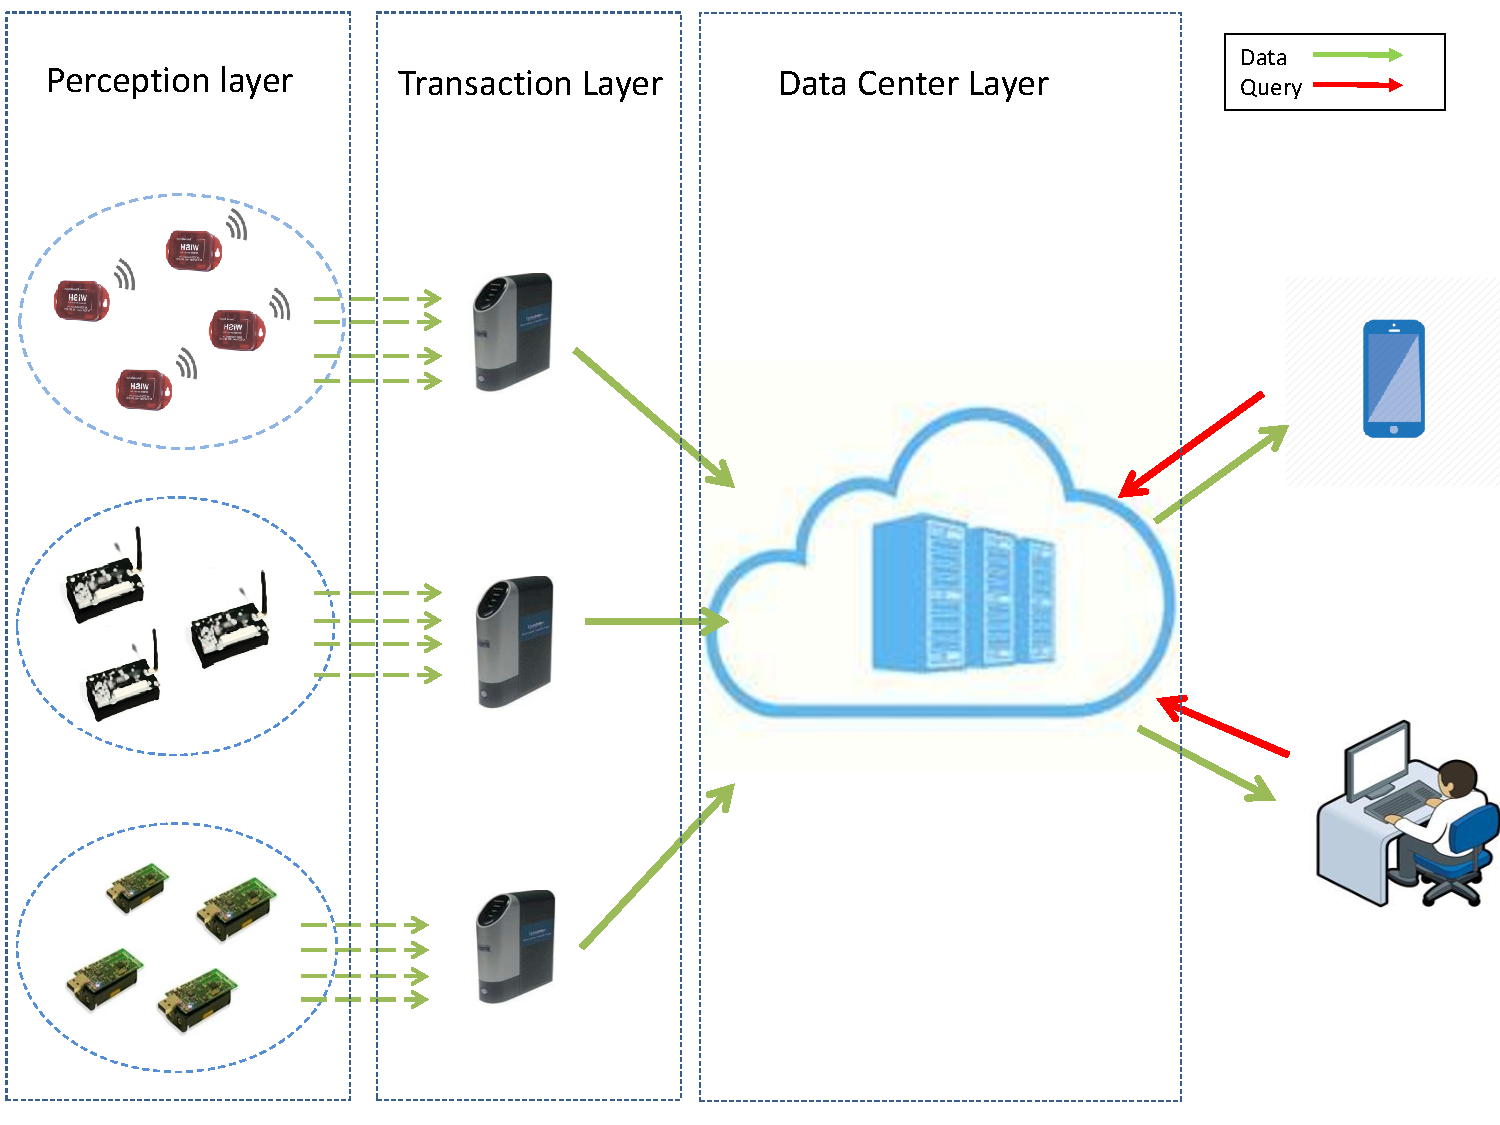
\includegraphics[scale=0.35]{/c4/c4-1-a-centralised.pdf}
    \caption{Architecture of a typical cloud-based IoT system.}
    \label{fig:4-1-a-centralised}
\end{figure}

In contrast to such centralised deployment, an edge-based system aims to push the data processing tasks away from a centralised node.
With the improvement of communication capability of the high-end IoT devices, they can be deployed as gateway nodes in the transition layer. 
Leveraging the advance of storage capability and computational power on such devices, data can be stored and queried from the gateway nodes.

\begin{figure}[ht!]
    \centering
    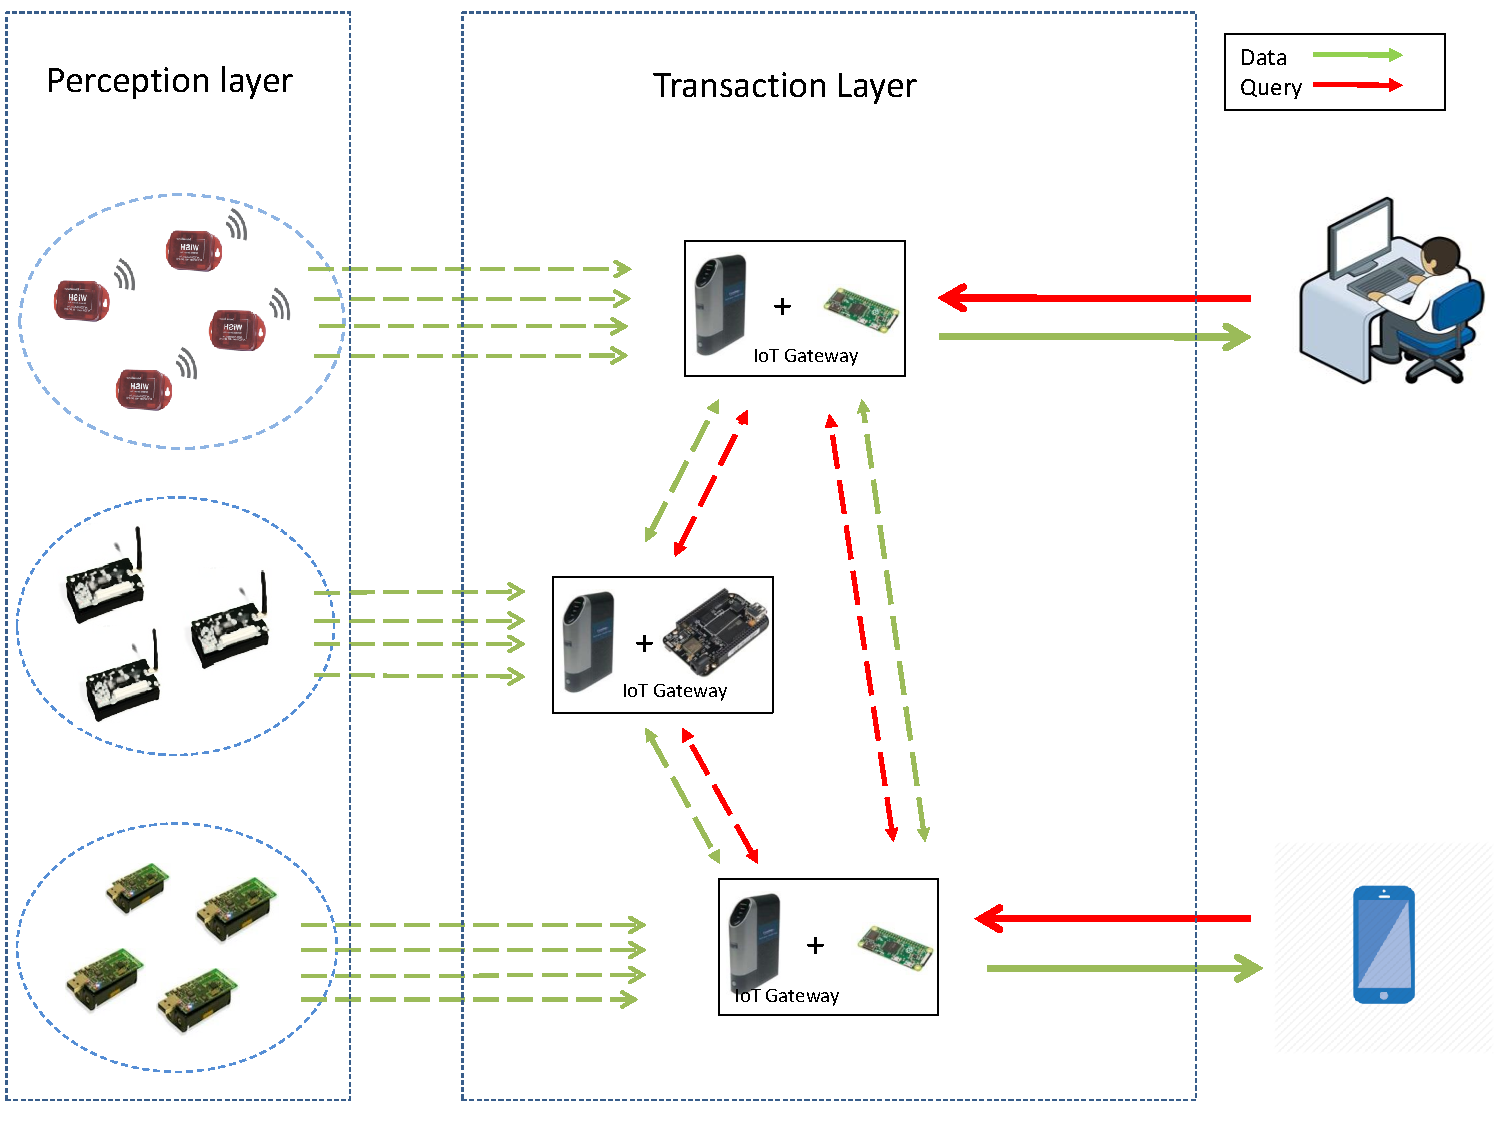
\includegraphics[scale=0.35]{/c4/c4-1-b-decentralised.pdf}
    \caption{Architecture of a typical cloud-based IoT system.}
    \label{fig:4-1-b-decentralised}
\end{figure}

The major challenge of such system is to enable the integration of the sensory data and the data federation between gateway nodes.
The information captured from each sensor device may be presented in a specific scheme, data structure.
Application may require to integrate the collected data which is stored on different gateway nodes.
Therefore, wrapper mediator architecture for data integration can be adopted to provide such integration and federation.
The working principle of such system is quit simple.
A wrapper converts data from specific data sources into objects of a common information model.
Queries from a mediator are transformed to queries understood by the sources and can be sent to other mediators.
The results are collected from the mediators and are merged before returning the answer.

In the scenario, Linked Data technologies is ideally a solution to deal with the heterogeneity of data and data sources.
Similarly to a typical deployment of an IoT system, in the perceived layer, 
the low-end devices (e.g., sensors, actuators) can be deployed across several sites in different locations (e.g., houses or weather stations).
The devices in the same site can be connected to a high-end devices which stand as gateway nodes. 
The RDF engines such as Jena TDB or Virtuoso can be brought to such devices to create such mediators. 
Physical data from low-end devices can be wrapped into RDF data and can be stored on the mediators using an RDF storage.
The federation mechanism of federated SPARQL queries can be also leveraged to provide the integration of mediators.
Simple data model of SPARQL federation such as RDF serialisation or SPARQL result can be used for information exchange between mediators.

\section{Evaluation}

In such edge-based system, the scalability of each edge nodes will contribute to the scalability of the whole system.
The more data can be handle from the edge node, the less likely data has to be sent outward networks.
With the growth of the Semantic Web, there have been many researches for scalable RDF data management.
The cloud-based RDF engines, such as ..., are able to handle billions to trillions of RDF triples.
On the common workstation, the RDF engines such as Jena TDB or BlazeGraph can efficiently store and query RDF dataset of hundreds of millions of RDF triples.
In this study, we aimed to investigate how much RDF data can be handle on the lightweight edge devices.

\subsection{DataSet}

For the evaluation, we used a generated RDF dataset that is similar to the Linked Sensor Data~\citep{}.
The real weather data was taken from the weather data dataset of NOAA's National Centers for Environmental Information(NCEI).
The weather data in this dataset was collected from around 20,000 weathers station in US.
On average, there are five sensors per weather station that measure the phenomena.
In order to describe the data in RDF format we used the updated version of SSN ontology~\footnote{https://www.w3.org/TR/vocab-ssn/}.

\begin{figure}[ht!]
    \centering
    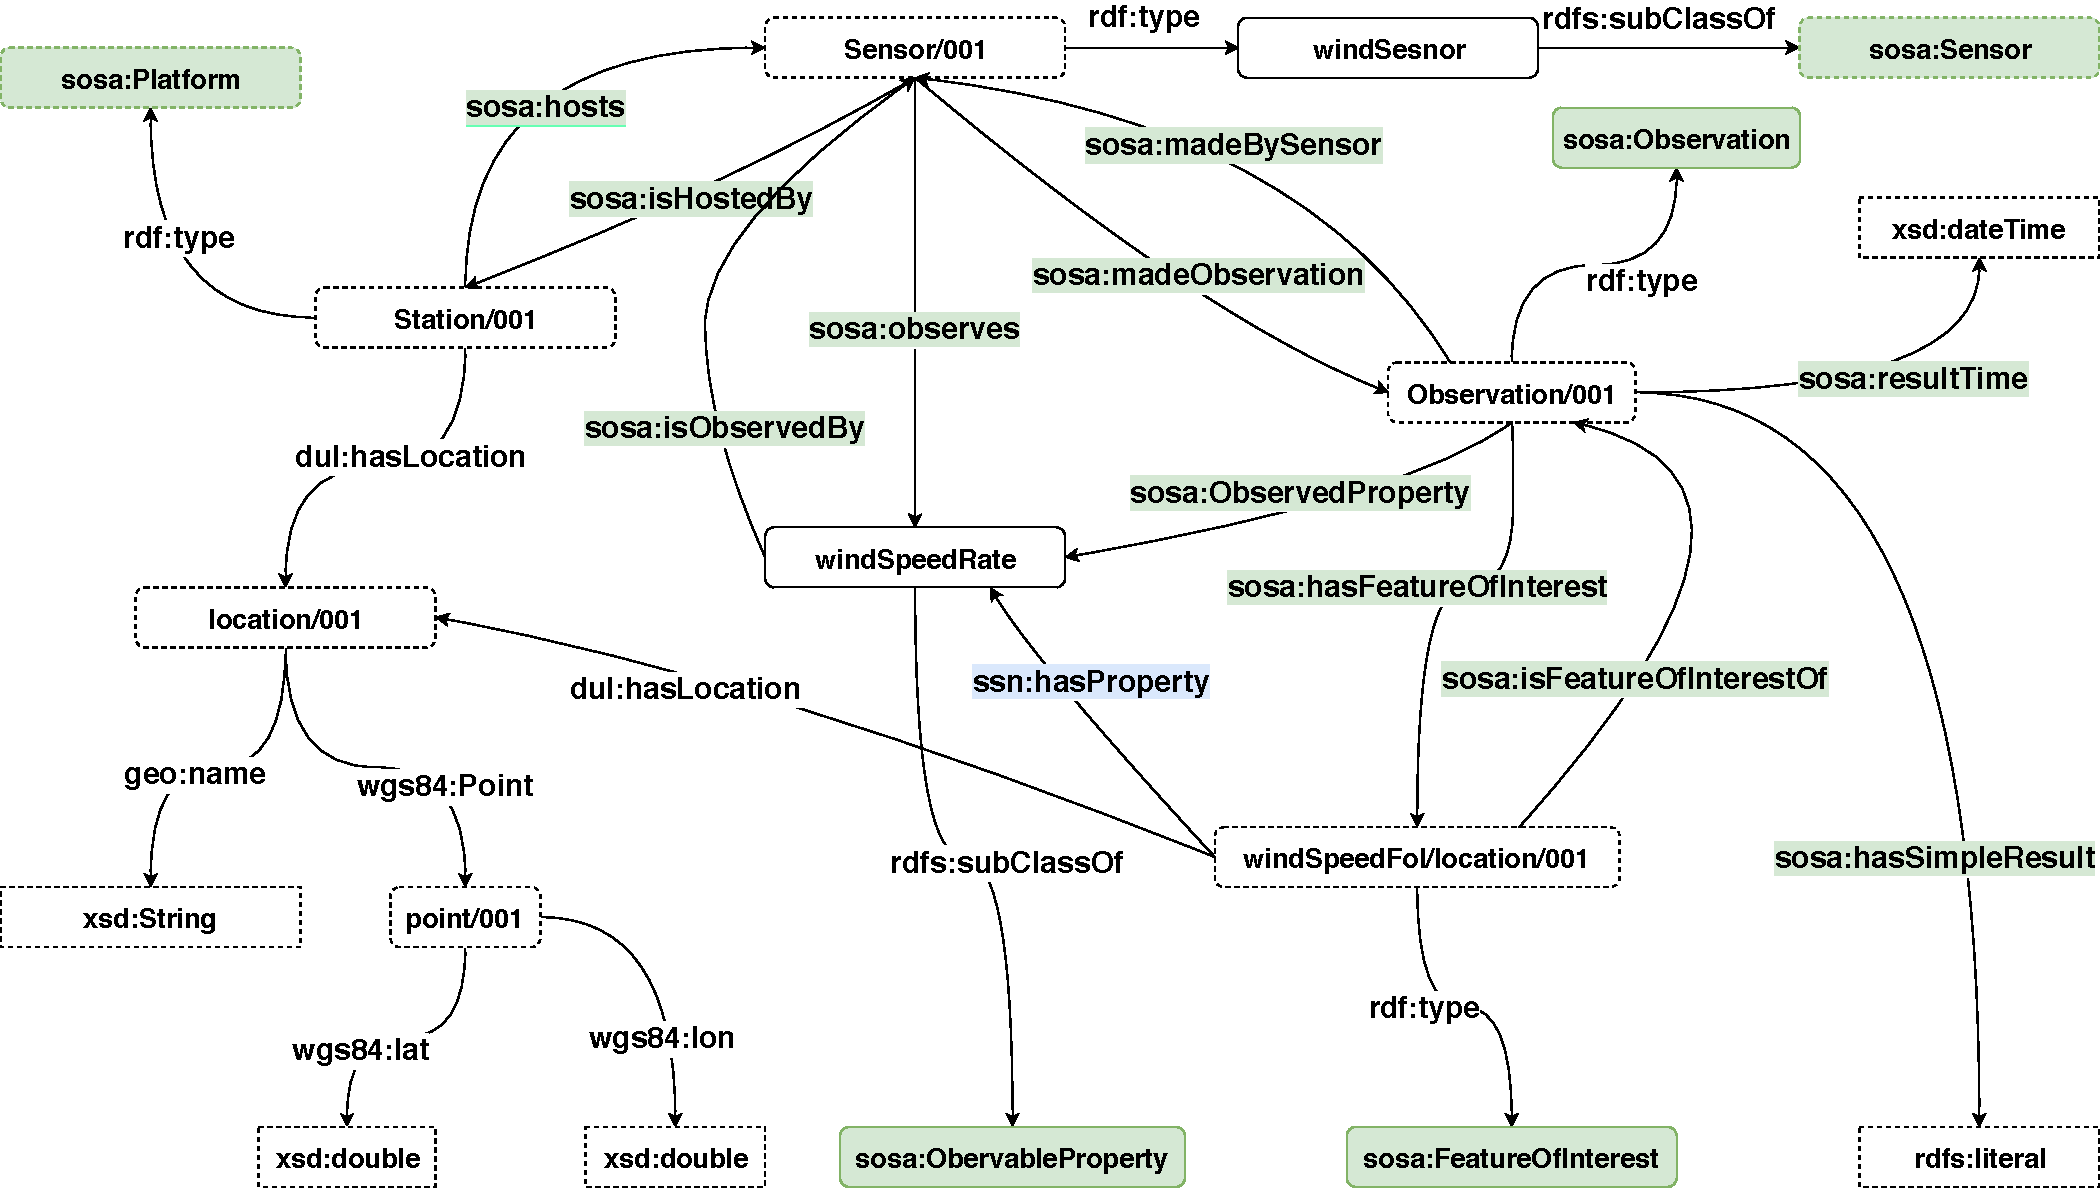
\includegraphics[scale=0.45]{/c4/c4-4-Schema}
    \caption{RDF schema for describing a weather station}
    \label{fig:4-3-weather-station}
\end{figure}

%\begin{figure}[ht!]
%    \centering
%    \includegraphics[scale=0.25]{/c4/c4-3-sensorSchema}
%    \caption{RDF schema for describing a weather station}
%    \label{fig:4-3-weather-station}
%\end{figure}

Figure~\ref{fig:4-3-weather-station} illustrates the RDF schema that describes a weather station.
Each weather station is represented by an URI and is defined as a system using \textbf{rdf:type} property and \textbf{ssn:System} class.
In consequence, a weather station has five sensors which are linked with the weather station using property \textbf{ssn:hasSubSystem}.
Each sensor has type \textbf{sosa:Sensor} and observes a specific \textbf{sosa:ObservableProperty}.
In addition to location attributes of weather station such as latitude, longitude, and geonames are also provided using GeoNames~\footnote{http://www.geonames.org/ontology/documentation.html} and WGS84~\footnote{https://www.w3.org/2003/01/geo/}.

The observations collected include measurements of phenomena such as temperature, visibility, precipitation, pressure, wind speed, humidity. 
The weather station’s observations also include the unit of measurement for each of these phenomena as well as the time instant at which the measurements were taken. 
The RDF schema that describes an observation, specifically wind speed, is illustrated in Figure~\ref{fig:4-3-observation}.
Each observation is linked to the sensor that made this observation using \textbf{sosa:madeObservation} and \textbf{sosa:madeBySensor}.
The phenomena is defined by the \textbf{sosa:FeatureOfInterest} class.
The observation is linked to its feature of interest using property \textbf{sosa:hasFeatureOfInterest} and \textbf{sosa:isFeatureOfInterestOf}. 
For example, the wind speed observation URI is connected to \textbf{windSpeedFOIIRI}.
The measurement unit of an observation is an plain literal, and time stamp of an observation is type literal.
They are connected to the observation using properties \textbf{sosa:hasSimpleResult} and \textbf{sosa:resultTime} perspectively.


%\begin{figure}[ht!]
%    \centering
%    \includegraphics[scale=0.35]{/c4/c4-4-observationSchema}
%    \caption{RDF schema for station metadata}
%    \label{fig:4-3-observation}
%\end{figure}

The example of using SPARQL query that extracts data from the sample dataset is presented in listing~\ref{lst:sparql_q1}.
The query is to request all wind speed measurement from station 1. 
The rest of the queries that are used in the experiment can be found in Appendix~\ref{}.

%====================================================================================
\begin{lstlisting}[
captionpos=b, 
language=sparql,
label={lst:sparql_q1},
basicstyle=\scriptsize\ttfamily,
caption={List all the wind speed values from a given station and order by time}]
PREFIX ssn:<http://www.w3.org/ns/ssn/>
PREFIX sosa:<http://www.w3.org/ns/sosa/>
PREFIX insight:<http://insight.org/dev/noaa/>

SELECT ?windSpeed ?time
WHERE
{
    insight:Station1 sosa:hasSubSystem ?sensor.
    ?sensor a sosa:Sensor.
    ?sensor sosa:madeObservation ?observation.
    ?observation sosa:hasFeatureofInterest insight:windSpeedFOIIIRI.
    ?observation sosa:resultTime ?time.
    ?observation sosa:hasSimpleResult ?windspeed.
}
ORDER BY (?time)
\end{lstlisting}


The measurements were read every half an hour and it is required 80 RDF triples to describe a measurement.
In order to store the data of a weather station in a year in active RDF graph on a gateway node, the RDF engine that runs on this node needs to store up to 1.5 millions RDF triples.
The dataset we used in the experiment was wrapped data from 20 workstation in year 2017.
The size of the dataset is 30 million triples.

\subsection{Hardware devices}

The experiments were conducted on three types of high-end IoT devices: Intel Galileo Gen II(GII), Raspberry Pi Zero W (Pi0), and Beagle Bone Black(BBB).
We chose these devices because they were popular and have been used for demonstrating the proof of concept of many researches in the IoT domain.
Furthermore, they are representatives for resource barriers of IoT gateways in our scenario in terms of size, memory and cost.

The Intel Galileo was developed by Intel and was the first IoT device that can run a complete Linux system.
The Intel Galileo was designed as hardware and software Arduino-compatible.
The design allowed Arduino sensors and actuators can be used out of the box on Galileo. 
Therefore, the Galileo hardware can be thought as composed by two set of hardware components which are the Arduino hardware and the "mini PC" hardware.
The Intel Galileo was equipped with RAM, Flash memory, mini SD card reader and Ethernet adapter.
Differently from the other boards, the Intel Quark x86 CPU was embedded on the board instead of the ARM CPU family.
Galileo came out with two versions: the Gen 1 Intel Galileo  and the Gen 2 Intel Galileo.
They are pretty similar, however, the Gen 2 boards had some hardware improvements.
Thus, we only use Galileo Gen 2 in our evaluation.

BeagleBoard was originally developed and introduced by Texas instruments in year 2008.
By using OMAP3530 System-on-a-chip technology, BeagleBoard boards were good platform to various demonstrating scenario in the researches of the IoT.
It was regarded as giant step that bring the microcontrollers to the full-fledged microcomputer. 
BeagleBone Black was a small credit card-sized BeagleBoard that was launched in 2013 at a price of $\$$45. 
Among other differences, on BeagleBone Black RAM was increased to 512 MB, ARM Cotex-A8 processor with the processor clock up to 1 GHz was equipped, and there was also 2 GB of eMMC flash memory on this small board. 

The Raspberry Pi was another the well-known, low-cost single board computer that was developed by the University of Cambridge.
Today, Raspberry Pi’s capabilities are similar to a PC, as it allows browsing the Internet, playing games, playing HD videos, working with word processing and spreadsheet applications. 
The Raspberry Pi is able to acquire information from sensors and interact with the actuators. 
The current models of Raspberry Pi are Model A+, Model B+, Pi 2 Model B and Pi Zero.
A Raspberry Pi Zero with smaller size  was released in 2015.
In 2017, the Raspberry Pi Zero W was launched, a newer version of the Zero with Wi-Fi and Bluetooth capabilities, for US$\$$10.
The Raspberry Pi runs Raspbian (a free operating system based on Debian Linux and optimized for the Raspberry Pi hardware). 

The configurations of each device are summarised on table~\ref{t:hc}. 

\begin{table}[ht!]
\centering
\begin{tabular}{ c | p{3.5cm} | p{3.5cm} | p{3.5cm} |}
\cline{2-4}
& \multicolumn{3}{c|}{Devices} \\  
\cline{2-4}
                                    & \multicolumn{1}{c|}{Pi0} & \multicolumn{1}{c|}{BBB} & \multicolumn{1}{c|}{GII}\\ 
\hline
\multicolumn{1}{|c|}{CPU}          & \multicolumn{1}{c|}{ARM 11,    1.0 GHz, 1-core }
								   & \multicolumn{1}{c|}{ARM A8,    1.0 GHz, 1-core }
                                   & \multicolumn{1}{c|}{x86 Quark, 0.4 GHz, 1-core } \\
\hline
\multicolumn{1}{|c|}{RAM}          & \multicolumn{1}{c|}{512 MB} & \multicolumn{1}{c|}{512 MB} &\multicolumn{1}{c|}{256 MB} \\
\hline
\multicolumn{1}{|c|}{Storage}      & \multicolumn{3}{c|}{Transcend MicroSD 16GB class 10 (40MB/s)} \\
\hline
\multicolumn{1}{|c|}{OS}           & \multicolumn{1}{c|}{Raspbian} & \multicolumn{1}{c|}{Debian 7.0} & \multicolumn{1}{c|}{Yocto} \\
\hline
\end{tabular}
\caption{Hardware Configurations}
\label{t:hc}
\end{table}

\subsection{RDF engines}
We run the experiment with three RDF engines that were able to set up on the three targeted devices: Jena TDB, Sesame, and Virtuoso.

Jena TDB is a component of Apache Jena, a Semantic Web framework that is available as open-source software.
Jena TDB is the persistent storage layer for Jena, and it works with Jena SPARQL query engine (ARQ) to provide complete SPARQL.
Jena TDB is a pure-Java implementation, employing memory mapped I/O, a custom implementation of B$^+$Trees.
TDB was tested with UniProt v13.4 (1.7B triples, 1.5B unique) on a single machine with 64 bit hardware.
It performed loading an average 12 thousands of triples per second.
In the experiment, Jena TDB version 3.5 was used.

Sesame is another Java-based open source framework for storage, inferencing and querying of RDF data.
Sesame includes RDF parsers and writers (Sesame Rio), a repository API for handling RDF data. 
It operates in any Java-supporting environment and can be used by any Java application.
Sesame provides native as well as RDB-backed triple storage. 
Sesame with ... was used.

Virtuoso is developed by OpenLink Software Inc, and it is a hybrid storage solution for a range of data models, including relational data, RDF and XML, and free text documents. 
Virtuoso has a RDB-backed storage, thus, it can be seen as an SPARQL-to-SQL solution for managing RDF data.
Virtuoso has gained significant interest since it is used to host many important Linked Data sets (e.g., DBpedia).
Virtuoso is offered as an open-source version and commercial version.
In this evaluation, we used Virtuoso 6 open-source version because Virtuoso 7 with column store was not able to be installed on 32-bit OS.

\subsection{Experiments}

We run three experiments to monitor the update throughput as we assume weather data should be collected in a sort interval of time, the query response time, and the memory consumption as memory is critical resource in such limited memory devices. The details of each experiment is presented as following:

{Exp1 - Update throughput:}
In the first experiment, we test how much new data the system can incrementally update with a certain underlying RDF store corresponding to each hardware configurations. 
We simulate the process of data growing by gradually adding more data to the system.
The metadata of 20 weather stations was inserted first and then the observation data.
We measure the throughput of inserting data (triples/second) until the system crashes or until the throughput is below 80 triples/second (whichever happened first).
When the system can not insert 80 triples/second, that means the system can not update 1 reading in a second.

{Exp2 - Query evaluation:} 
In the second experiment, we test the queries response time of each engine.
On each device, we chose the size of the dataset with the scale that all the engines can store.
We followed the approach of WATDIV benchmark to create queries with different shapes: linear, star or snowflake.
The set of queries can be found in the Appendix~\ref{}.
We recorded the maximum, the minimum and the average time that the engines answer each type of queries.

{Exp3 - Memory consumption:}
In the third experiment, we measured the memory consumption of three system configurations while performing the insertion and query.  
The experimental application ran the different queries repeatedly and recorded the maximum memory heap that the operating system allocated for it. 
Note that the memory consumption is device-independent. 
To evaluate the impact of the data size on memory consumption, the test was conducted on the BBB with 15 datasets and with different sizes.dataset. 
The scale ranges from 2 million triples to 50 million triples. 

\section{Result}

\subsection{Insert Throughput}


\newpage

\begin{figure}[ht!]
    \centering
    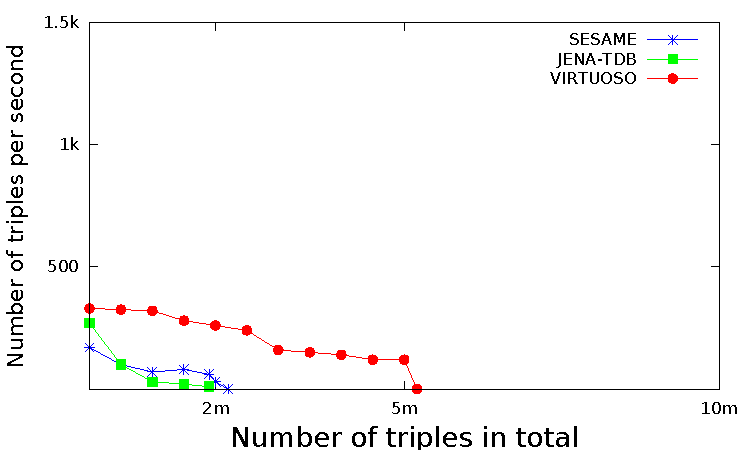
\includegraphics[scale=.85]{/c4/c4-GII-input}
    \caption{Insert throughput on Gallileo Gen II}
    \label{fig:4-3-GII}
\end{figure}

\begin{figure}[ht!]
    \centering
    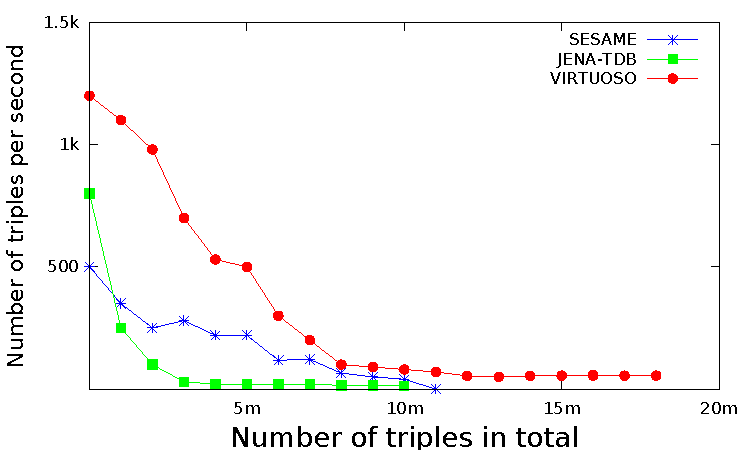
\includegraphics[scale=.85]{/c4/c4-BBB-input}
    \caption{Insert throughput on BeagleBone Black}
    \label{fig:4-3-BBB}
\end{figure}

\begin{figure}[ht!]
    \centering
    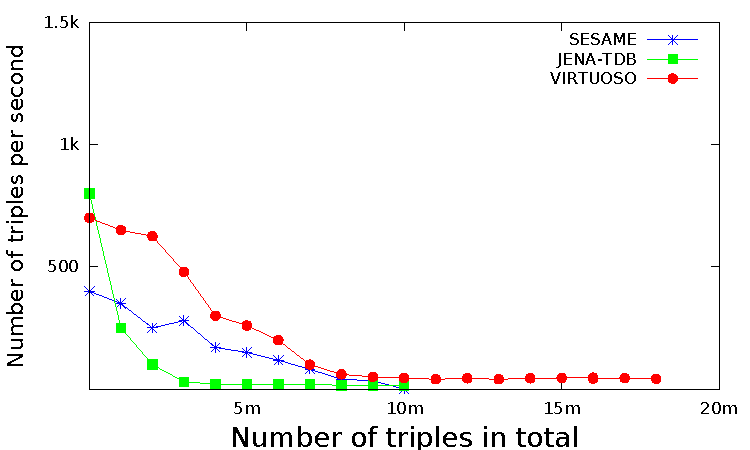
\includegraphics[scale=.85]{/c4/c4-PI0-input}
    \caption{Insert throughput on Raspberry Pi Zero}
    \label{fig:4-3-PI0}
\end{figure}
\newpage


\subsection{Query Response Time}

\newpage
\subsection{Memory Consumption}

\begin{figure}[ht!]
    \centering
    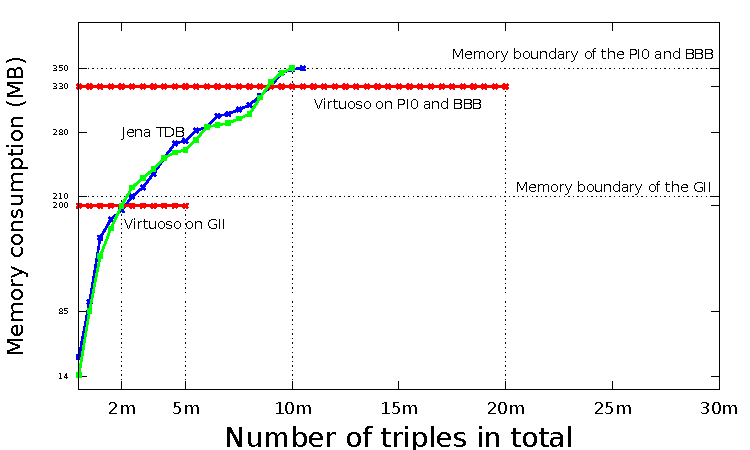
\includegraphics[scale=.85]{/c4/c4-input-mem}ifc
    \caption{Insert throughput on BeagleBone Black}
    \label{fig:4-3-BBB}
\end{figure}

\begin{figure}[ht!]
    \centering
    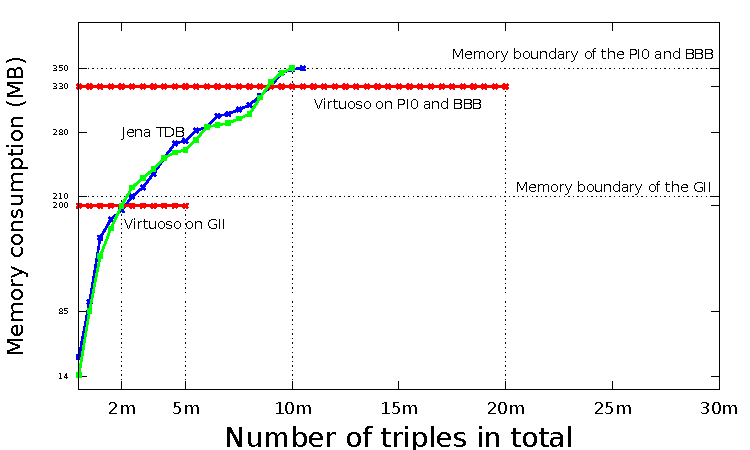
\includegraphics[scale=.85]{/c4/c4-query-mem}
    \caption{Insert throughput on Raspberry Pi Zero}
    \label{fig:4-3-PI0}
\end{figure}
\newpage

\section{Discussion}























 
%%\chapter{Rationale of Designing RDF engine for Edge nodes}






\chapter{Flash-Aware RDF Storage}
\label{ch:rdfstorage}
\lhead{Chapter~\ref{ch:rdfstorage}. Flash-Aware RDF Storage}


This section provides the design of physical organisation of RDF storage for IoT edge devices.

%---------------------------------------------------------------------------------%
\section{Architecture Overview}
\label{s:ao}
\lhead{\ref{s:ao}. Architecture Overview}


\begin{figure}[ht!]
   \centering
   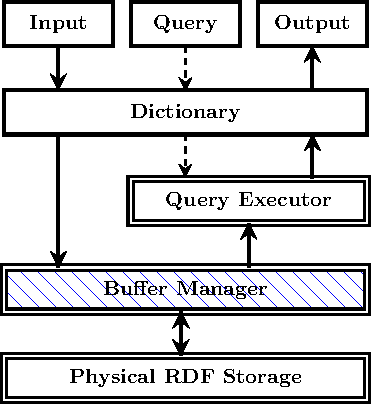
\includegraphics[width= 0.35\textwidth]{c5/arch}
     \caption{System Architecture Overview}
   \label{fig:arc_ove} 
\end{figure}




\section{RDF Physical Storage Design}
\label{sec:c4-retionale}

The physical organisation heavily influences the write performance, read performance and space utilisation of a database~\citep{Ullman:2001}. 
The selection of physical organisation for a database is also impacted by the type of storage medium that the database targets~\citep{Owens:2011}.
From the findings in Chapter~\ref{}, the schemes for storing RDF data on a workstation -- as described in Section~\ref{} -- cannot be deployed on the IoT edge devices.
Therefore, it is required to design an alternative physical organisation for RDF data that is well-suited the characteristic of hardware characteristic of IoT edge devices (presented in Section~\ref{}) and also provides high insert throughput for the RDF engines.

As we already mentioned in Section~\ref{}, RDF triples can be stored following the approach of multiple-indexing techniques~\citep{}.


%In order to store RDF data, we following the approach of creating access patterns for RDF triples as described in Section~\ref{sec:phy_sto}. For every RDF graph(dataset), three Triple lists, namely subject-predicate-object (SPO), predicate-object-subject (POS), object-subject-predicate (OSP), are created. 
%With this schema, for any combinations of subject, predicate, or object, a corresponding list, which is suitable for retrieving related triples, can be found in these three lists. Several RDF stores do implement all six of the possible indexing orderings over RDF data such as Hexastore~\cite{Weiss:2008} or YARS~\cite{Harth:2005}. However, using three combinations of nodes in a cyclic ordering is enough to cover all query patterns. This indexing schema is not efficient for answering complex queries~\cite{Weiss:2008}; however, to compare with other schemes, this costs lower resource for updating and consumes smaller storage space.


Following the approach of multiple-indexing, RDF4Led
stores RDF triples in three storage layouts as sorted permu-
tations of triples: SPO (Subject - Predicate - Object), POS,
and OSP. 
Three permutations are sufficient to cover all query patterns, e.g., the SPO layout can be used to cover the triple query patterns with the bound subject (s ? ?) and the bound
subject-predicate (s p ?). 
Although, storing all six combinations may answer complex queries more effectively, using only three consumes less storage space and decreases the cost of updates, i.e., we must update only three data structures instead of six, which is crucial for flash storage.

To reduce the memory required to maintain the index of data in flash storage, we use an alternative index structure that is based on the Block Range Index(BRIN) approach [20]. 
The basic idea of BRIN is to summarise the information of a data block of persistent storage (e.g. its location) into a small tuple. 
The result is that we minimise the amount of memory required to maintain the index of the data.


Specifically, we introduce a \emph{Physical Layer} and a \emph{Buffer Layer}. 
The Physical Layer stores data directly on flash storage (Physical RDF Storage) and the Buffer Layer operates in the main memory (Buffer Manager) and has the following main roles: 
\begin{itemize}
\item (i) grouping and caching atomic data updates before writing a block; 
\item (ii) indexing the data stored on the Physical Layer 
\item (iii) caching recently used data for read performance. This allows us to group multiple updates within a block into one erase-and-write operation and to improve read performance through the cache.
\end{itemize}

\begin{figure}[ht!]
	\centering
    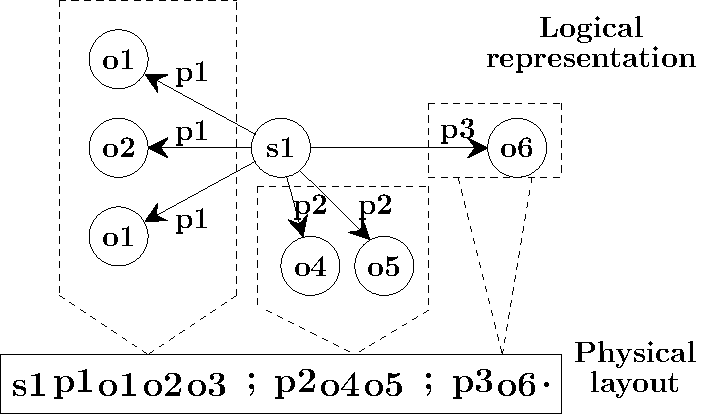
\includegraphics[width=0.5\textwidth]{c5/molecule.pdf}
    \caption{Logical and physical representation of a molecule.}
    \label{fig:molecule}
\end{figure}

\subsection{Physical Layer:}  

To achieve high compression of triples on the flash storage we leverage the molecule-based storage model. 
RDF molecule is a hybrid data structures, it stores a compact list of properties and objects related to a subject, i.e., the root of the molecule.
Molecule clusters are used in two ways: to logically group sets of relates resources, and to physically co-locate information related to a given object. 
Physically we represent a molecule as a list of co-located integers corresponding to S, P, and O (Figure~\ref{fig:molecule}). 
In such a way, we avoid storing repetitive values multiple times. Moreover, we enable further data compression, e.g., by storing deltas of sorted integers instead of full values.


In Physical Layer, we store sorted molecules into contiguous pages (read units) which are grouped into blocks (erase units). Moreover, all entities in molecules are also sorted to improve search performance. In this example depicted on Figure~\ref{fig:index}, each block in the Physical Layer contains four pages and each page stores molecules. 

\subsection{Buffer Layer:}

Similarly to the idea of BRIN, the Buffer Layer summaries the information of the data in the Physical Layer.
In the Buffer Layer, we keep the information about the first triple of a molecule in a page and the first page in a block. Figure~\ref{fig:index} depicts an example of the indexing structure that uses for storing an SPO index. The Buffer Layer maps physical addresses of pages and blocks, thus it acts as an index for the Physical Layer. We distinguish three types of an entry in the Buffer Layer: tuple entry, page entry and block entry. A \emph{page entry} is an entry that refers to the beginning of a page in the Physical Layer, it contains the first triple in the first molecule of the page. A \emph{block entry} is a page entry with an extra field indicating that this page is the first page a block. A \emph{tuple entry} contains an atomic triple and a value indicating whether this triple has been modified. In the Figure~\ref{fig:index}, the gray columns represent block entries and white columns represent page entries. For fast lookups on Buffer Layer, all triples are sorted.  Moreover, we maintain the logical order of the triples as in the Physical Layer. This allows us to group and commit sequential pages containing modified triples and belonging to the same block, within one write operation.

\begin{figure}[ht!]
\centering
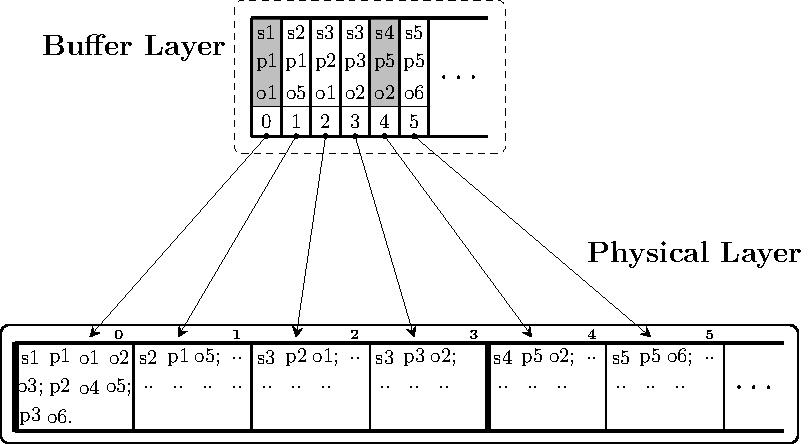
\includegraphics[width=.7\textwidth]{c5/index.pdf}
\caption{Two-layers storage model consist of a Physical Layer and a Buffer Layer.}
%The Physical Layer stores data on flash storage in a form of compact molecules.}
%The Buffer Layer manages changes in data,  caches changes in main memory, indexes data on Physical Layer, and caches data for reads. The Buffer Layer manages changes in data,  caches changes in main memory, indexes data on Physical Layer, and caches data for reads.
\label{fig:index}
\end{figure}

%---------------------------------------------------------------------------------%
\section{Index lookup} 

To retrieve RDF triples that match a triple pattern we execute a lookup on a corresponding layout of molecules. For example, a triple pattern (s, p, ?) is executed on the SPO layout or a triple pattern (?, p, o) is executed on the POS layout. As triples are sorted, the matched tuples are retrieved as a sublist. For instance, the matched tuples of the triple pattern (s, p, ?) are the tuples on the SPO layout which are of a form (s, p, o$_{i}$) and they are located between (s, p, o$_{min}$) and (s, p, o$_{max}$), where o$_{min}$ and o$_{max}$ are the smallest and the greatest object's identifiers within the layout. In other words, the sublist is computed by finding the lower and the upper bound positions of the matched tuples on the layout.
As in the example, the lower bound position of the matched sublist is the position of the tuple (s, p, o$_{min}$) and the upper bound position is the position of the tuple (s, p, o$_{max}$).
The matched triples are extracted from the layout by probing the range tuple by tuple from the lower to the upper bound positions. 

A position of a tuple is identified with a page, a molecule, and the exact position of the tuple within the page. To search for the lower bound position, we replace variables of the triple pattern with Integer$_{min}$ (the minimal integer value that can be used as an ID) and we do a simple search with the tuple. For the upper bound, we replace the variables by Integer$_{max}$ (the maximal integer value that can be used as an ID).
The search first finds the page that contains the tuple by searching in the Buffer Layer. 
The page entries within the Buffer Layer points to the first triple of the first molecule of each page, such entries are also sorted. Therefore, to find a page we perform a binary search over the page entries in the Buffer Layer. Then, we read the page from the Physical Layer and we perform the second binary search to find the exact position of the tuple within the page. 

For instance, to lookup of triple query pattern (09, ?, ?) is executed on the SPO layout depicted on Figure~\ref{fig:index}. The first tuple of the sublist is the first tuple that is greater than or equal to the triple (09, Integer$_{min}$, Integer$_{min}$) and the last tuple of the list is the first tuple that is smaller than or equal to the triple (09, Integer$_{max}$, Integer$_{max}$). 

With binary search over the Buffer Layer, we determine the physical pages containing the boundaries of the sublist:

\begin{itemize}
\item the lower bound within page 2 since (08, 07, 09) on the is the first tuple smaller than (09, Integer$_{min}$, Integer$_{min}$), and the page 3 starts already a tuple that is greater than (09, Integer$_{min}$, Integer$_{min}$) , i.e., (09, 05, 10);
\item the upper bound within page 8, since (09, 13, 01) is the first tuple smaller than  (09, Integer$_{max}$, Integer$_{max}$) and page 9 starts with a tuple greater than (09, Integer$_{max}$, Integer$_{max}$), i.e., (15, 6, 16). 
\end{itemize}

To find the exact positions of the lower and the upper boundaries we perform a second binary search withing pages 2 and 8. We find that the lower bound is on the second position within the  page 2. In case where tuple (09, Integer$_{min}$, Integer$_{min}$) was greater than the last tuple of page 2, the binary search would continue from the first tuple of page 3. Then, we find that the upper bound is on the first position within the  page 8. The last tuple of page 8 cannot be greater that (09, Integer$_{min}$, Integer$_{min}$) because in the Buffer Layer it is shown that the page 9 starts with (15, 06, 16). 
In consequence, we determine the physical boundaries of the sublist with tuples for our triple patterns (09, ?, ?) as: 

\begin{itemize}
\item the lower bound - the second position within the page 2
\item the upper bound - the first position within the page 8
\end{itemize}

In order to retrieve the results, we first load to the Buffer Layer the pages corresponding to the lower bound of the sublist, the triples from this page are then read one by one starting from the lower bound position. Then, we execute a similar process for all consecutive pages indicated by the page entities up to the page corresponding to the upper bound of the sublist. The process is halted at the position of the upper bound within the last page. The intermediate pages contribute to the results with all their triples. For our example, we load page 2 to the Buffer Layer, and we start retrieving triples from the second position of this page (the lower bound), then we load page 3 and we retrieve all its triples (intermediate page). Finally, we load page 8 and we retrieve only its first triple (the upper bound).

\section{Write Manager}

The write from Buffer Layer to Physical Layer is managed to adapt to the I/O behaviors of flash memory by the following basic principles: (i) minimise the number of physical writes to physical storage; (ii) group multiple updates within one write operation; (iii) keep a relatively high hit ratio for the data in the buffer. We use the Buffer Layer to delay write operations and to group many updates in blocks, hence, to mitigate the issue of single erase-before-write operations. For the high hit ratio, we keep the data block with the higher chance to be accessed and modified in the future. 

In order to keep track on the access frequency among blocks, we divide the buffer into two parts: cold and hot. In the hot part, we keep blocks that have been recently accessed, hence we do not want to move them to the Physical Layer. We organize data in a flat fashion within the hot part, i.e., we keep sorted triples instead of molecules to speed up atomic updates. The cold part contains molecule blocks that can be moved to the Physical Layer. When we access a block from the cold part or from the Physical Layer, we place it in the hot part of the Buffer Layer. 

The blocks are released from the hot part to the cold part and from the cold part by the following prioritised 
criteria: (i) the clean/unmodified blocks; (ii)the block with higher number of atomic triples in buffer; (iii) the higher density blocks, define by the ratio between the number of triples in a block and the capacity of the block i.e: $density_{Block A} = \frac{\#triples_{Block A}}{capacity_{Block A}}$; (iv) the last recently used blocks.   

\begin{figure}[ht!]
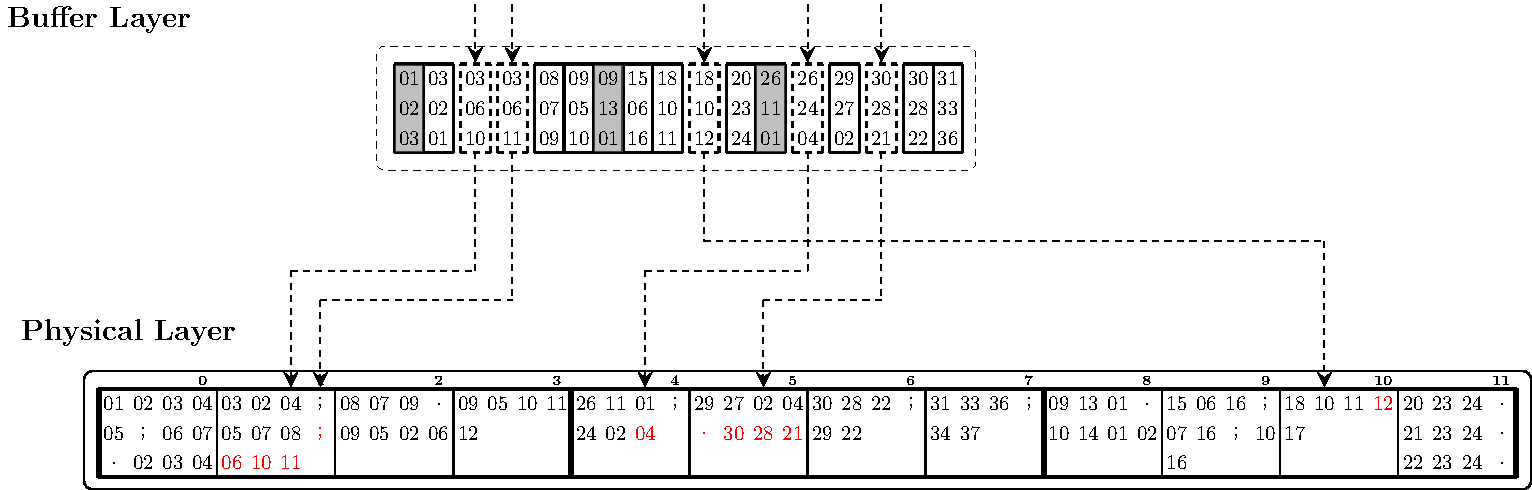
\includegraphics[width=1\textwidth]{c5/insert.pdf}
\caption{Example of inserting}
\label{fig:insert}
\end{figure}

Such order allows us to keep dirty/modified blocks in the buffer as long as possible in order to delay write operations and group more updates within dirty blocks. In case we need to release memory, we always refer to the cold part and we begin from the begin of the priority list. In consequence, we prioritize clean/unmodified blocks, as we do not have to perform any write operation for them, we just release the memory they occupy. Then, we prioritise blocks that contain many triples, i.e., high-density blocks, as they group multiple updates into one erase-write operation. 

For example, in Figure~\ref{fig:insert} illustrates the process of inserting 5 triples (03, 06, 01), (03, 06, 04), (18, 10, 12), (26, 24, 04), and (30, 28, 21). We first add them to the Buffer Layer; the page entries in the Buffer Layer indicate pages where the triples will be physically inserted. Triples (03, 06, 01), (03, 06, 04) are lexicographically smaller than the triple (08, 07, 09) which is the page entry mapping page 2 hence, they are added to page 1. Similarly, triple (18, 10, 12), (26, 24, 04) and (30, 28, 21) are will be added respectively to page 10, page 4, and page 5. 

When the size of the Buffer Layer reaches its limit or when data need to be moved to free memory, the triples are written to the Physical Layer. All dirty pages, i.e., pages containing modified tuples, within the same block are written at the same time to same expensive erase operations. For example, when the system needs to write 2 triples from buffer to storage, we move either data belonging to block 0, i.e., triples (03, 06, 01), (03, 06, 04), or data belonging to block 1, i.e., triples (26, 24, 04), (30, 28, 21), so that only one block is erased. In case we choose tuples (18, 10, 12) and (30, 28, 21), the system would have to erase two blocks before writing the data. Moving data from the Buffer Layer to the Physical Layer is essentially an optimization problem of maximizing the number of triples we can write within the minimal number of blocks in order to minimize the number of erase operations. Of course, block 0 is written before block 1 as its density is greater than that of block 1. The higher density means the less chance that the next triple will be dropped into that block.




\section{Evaluation Result}

\section{Summary}


%\section{Summary}


%As emphasized in the previous chapter, the design of existing mobile RDF triplestores exhibits several problems for the efficient storage and retrieval of RDF data on mobile devices. These designs are due to a lack of awareness of the small memory on mobile devices or distinctive I/O behaviour of flash storage. In order to overcome such issues, we consider creating a new design for mobile RDF triplestores.


%This chapter outlines our design for an efficient mobile RDF triplestore and improved techniques and strategy for storing RDF data. 
%Our design takes consideration from the ...
%he overview architecture of the mobile RDF triplestore and its building blocks are briefly described in Section~\ref{sec:c4_arch_overview}. In Section~\ref{sec:node_dic}, we discuss our strategy for reducing the memory consumption for representing RDF data in main memory by using an encoded dictionary. The selected physical organisation of mobile RDF storage is depicted in Section~\ref{sec:phy_org}.





























\nop{
Regarding the I/O cost of HERMES, suppose that available memory is M memory pages.
During the merging phase, M −1 memory pages are used for reading the input and 1
page is used to write to the output run. If the total size of the input tree is T memory
pages then each initial run will have an average size of 2(M − 1). Also, since
M − 1 buffers can be used for merging, there are going to be dlogM−1
d
T
2(M−1)
ee levels
of merging. Adding the first pass over the input to create the initial runs, we
have that there will be 1 + dlogM−1
d
T
2(M−1)
ee passes over the input. In each of these
passes, the whole tree is read and written to disk. This makes a total I/O cost of
2T ·

1+dlogM−1
d
T
2(M−1)
ee
.
As pointed out in [Graefe, 1993], one of the main concerns with replacement selection
is how one can handle the payloads of the nodes that reside in main memory
at any given time, i.e., the payloads of the nodes whose keys are in the heap at that
time. If these nodes are kept in the original buffer pages there is a great waste of space:
only half of the nodes of any given page are expected to be in the priority heap of their
parent node at any given point in time. This would mean that half of the available
memory is not effectively used for sorting keys. Therefore, the benefits from replacement
selection are cancelled (and quicksort could be used instead, probably yielding
better results). As also pointed out in [Graefe, 1993], the solution to this problem is
to copy the payloads of those nodes to a temporary space in memory until they are
written to the run, so that no space is wasted. Assuming that nodes of the same type
have similar size, this can be a viable solution. However, large variations in the size
of the nodes of the tree require complex and potentially overhead-inducing in-memory
management primitives.

Double buffering certain pages during the merging process is also a technique that
can improve the performance of our algorithm. For instance, using more than one
memory pages for the output run at each merge level can eliminate the need for the
CPU to wait for a write I/O call to complete after the output buffer is flushed (as is
the case if a single output buffer is used). Regarding the input buffers, the situation
is somewhat different. Reserving two memory pages (or more) per input run would
reduce the number of runs we can merge by half. What we can do is reserve a number
of k memory pages in order to prefetch the next page from the k input buffers that
contain one of the k smallest maximum keys among all buffers (since we then know
that the next page to be read will be the next from one of those k runs).

}




%\chapter{Adaptive Strategy for Iterative Join Execution}
\label{sec:adapt}

The most resource-intensive task of answering a SPARQL query is to perform the graph pattern matching over the RDF dataset. 
The graph matching operator executes a series of join operations between RDF triples that matches the triple patterns. Join operations have the greatest impact on the overall performance of a SPARQL query engine, typically requiring a large number of comparison operations that can only be done efficiently if records are stored in memory. 

\section{Join Propagation Algorithms}

The join performance can be tuned by optimisation algorithms which plan optimal join orders and join algorithms~\cite{Stocker:2008,Neumann:2008,Tsialiamanis:2012}. 
These approaches assume that memory is always available during the course of the execution of a chosen query plan. However, in  light-weight computing devices memory is critically low and, as such, the memory resource available for an RDF engine is unreliable, e.g. a surge of number network connections to the device might drain out available memory for all other running processes. Lack of memory may block  join operations that require temporary virtual memory such as hash-joins or sorted-merge joins,  and thus hurts the overall performance of the query engine or probably crashes the engine.

Materialisation techniques that write intermediate join results to storage is an attractive solution for the issue of  memory shortage~\cite{Garcia-Molina:2008}. However, on flash storage, writing is much slower if a random write happens. Furthermore, a limited number of erase operations can be applied to a block of flash memory before it becomes unreliable. 

To minimise the memory required  to execute a SPARQL query making the best usage of the indexing scheme introduced in Section~\ref{sec:index}, we adopt the \textit{one-tuple-at-a-time} paradigm to compute the join. This approach can reduce the memory consumption as no virtual temporary memory is required to buffer the intermediate join results. 
The basic idea of the algorithm to compute the join of a graph pattern is as follows.
A mapping solution (mapping for short) is continuously sent to visit each triple pattern of the graph pattern.
In each visit, it searches for triples matching with the triple pattern.
For each matched triple, variables in the triple pattern and the corresponding value in the triple are added to the mapping.
The mapping with new values will be sent to visit the next triple pattern, or be returned as query result when all triple patterns have been visited.

%===================================================================================================
\begin{algorithm}[ht!]
\label{alg:jp}
\caption{Join propagation}
	\SetKwProg{Fn}{Function}{}{end}
	\SetKwFunction{fn}{findNextPattern}
    \SetKwFunction{eval}{eval}
    \SetKwFunction{bind}{bindMapping}
    \SetKwFunction{reset}{resetMapping}
    \SetKwFunction{isCompatible}{isCompatible}
    \SetKwFunction{jp}{propagate}
    \SetKwInOut{Input}{input}
    \SetKwInOut{Output}{output}
     
    \Fn{\jp{$\mu$, $\mathbb{P}$}}
    
    \Input{$\mu$        : mapping, 
           $\mathbb{P}$ : set of triple query patterns}
           
    \Output{$\mu$ : mapping} 
    
    \If {isEmpty($\mathbb{P}$)}
    {
      	\Return $\mu$;
    }
    
    $p    \leftarrow$ \fn{$\mu, \mathbb{P}$}\;
    $p_{key}     \leftarrow  createKey(\mu, p)$\;
	$\mathbb{T}  \leftarrow$ indexScan($p_{key}$)\;
    $\mathbb{P}' \leftarrow$ $\mathbb{P}\setminus\{p\}$\;
    
    \For{$t$ $\in$ $\mathbb{T}$}
    {
    	$\mu$ $\leftarrow$ \bind{t, $p$}\;
      	\jp{$\mu$,  $\mathbb{P}'$}\;
        $\mu$ $\leftarrow$ \reset{t, $p$}\;
    }
\end{algorithm}
%=================================================================================================================


The abstract of the join propagation algorithm is given in the Algorithm 1. The propagate($\mu$, $\mathbb{P}$) function  is used to recursively propagate the input mapping. 
The function starts with an empty mapping $\mu$ and a set of unvisited triple patterns $\mathbb{P}$.
For each run, it checks and returns the input mapping as a result if there is no triple pattern left to visit (line 1-2). Based on the given input mapping, it looks for the optimal unvisited triple query pattern to visit (line 3). 
To search for triples compatible with pattern p, an index search key $p_{key}$ is created by replacing the variables in p according to $\mu$ (line 4). 
For each matched triple \textit{t}, the corresponding variables and values are bound into the mapping. Then another propagation of the mapping to the remaining unvisited triple patterns is called (line 7-10).

In each run of the propagation algorithm, the function findNextPattern($\mu$, $\mathbb{P}$) is called to find the optimal triple pattern to execute the propagation (see Function 1).
For each triple pattern \textit{p} in $\mathbb{P}$, the set of triple query patterns , the function searches for a triple pattern that shares variables with the input mapping $\mu$ at line 4. With each shared pattern found, an index search key pattern, $p_{key}$, is created (line 5). An index lookup on  $p_{key}$ is executed to search for the upper bound and lower bound positions of the set of the matching triples in the index, as described in the previous section (line 6). The size of the index lookup $\mathbb{I}$ is defined as the range between the upper bound and  lower bound positions (lined 7-9). The function returns the triple pattern that has the minimal size of the index lookup at line 11.


\section{Routing Policy}

%================================================================================================================================
\begin{function}[ht!]
\caption{1: findNextPattern($\mu, \mathbb{P}$)}
\SetKwProg{Fn}{Function}{}{end}
    \SetKwFunction{findNextPattern}{findNextPattern}
    \SetKwInOut{Input}{input}
    \SetKwInOut{Output}{output}
     
    %\Fn{\findNextPattern{$\mu$, $\mathbb{P}$}}
    
    \Input{$\mu$ : mapping, $\mathbb{P}$ : set of triple query patterns}
    \Output{P : triple query pattern} 
    
    $p_{next}\leftarrow null$\;
    $s_{min}\leftarrow Integer_{max}$\;
    
    \For{p $\in$ $\mathbb{P}$}
    {
      \If{isShared($\mu$, p)}
      {
		$p_{key} \leftarrow  createKey(\mu, p)$\;
        $I       \leftarrow  indexLookUp(p_{key})$\;
        $s       \leftarrow  sizeOf(I)$\;
        
        \If{$s < s_{min}$}
        {
           $s_{min}\leftarrow s$\;
           $p_{next}\leftarrow p$\;
        } 
      }
    }
    \Return $p_{next}$\;
\end{function}
%================================================================================================================================

The join propagation algorithm is similar to the nested iterations. Nested loop join is often argued to give poor performance as it does not attempt to prune the number of comparisons. However, equipped with an efficient index scheme, an index nested loops join can perform as well as other join algorithms~\cite{Graefe:2003}.
With the design of our storage, the index lookup can be done mostly within the buffer layer, only two extra I/Os may be required. The visitor pattern, that sends a mapping to visit each triple pattern and to execute index lookup, reduces the extra memory for the joins as only a mapping is kept in the main memory. This mechanism also enables the adaptivity for the joins. The function findNextPattern($\mu, \mathbb{P}$) decides which triple pattern the mapping should visit first. Similarly to routing policy of the stream processing engines, e.g Eddies~\cite{Avnur:2000} or CQELS~\cite{Danh:2011}, this function defines the propagating policy to achieve a certain optimisation purpose. In our case, we attempt to minimise the number of the propagations by choosing the shortest index scan in each run. Note that, this is the key place holder to add sophisticated optimisation algorithms, e.g. adaptive caching algorithm to be discussed in our future work.  

\section{Cost model}

\section{Evaluation}


\begin{figure}[ht!]
\centering
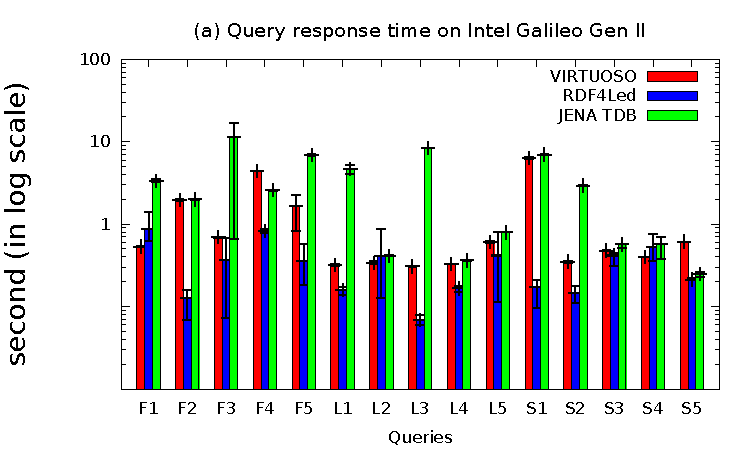
\includegraphics[width=0.3\textwidth]{c6/GII_QUERY_WATDIV_20.pdf}
\label{fig:result_query}
\end{figure}

\begin{figure}[ht!]
\centering
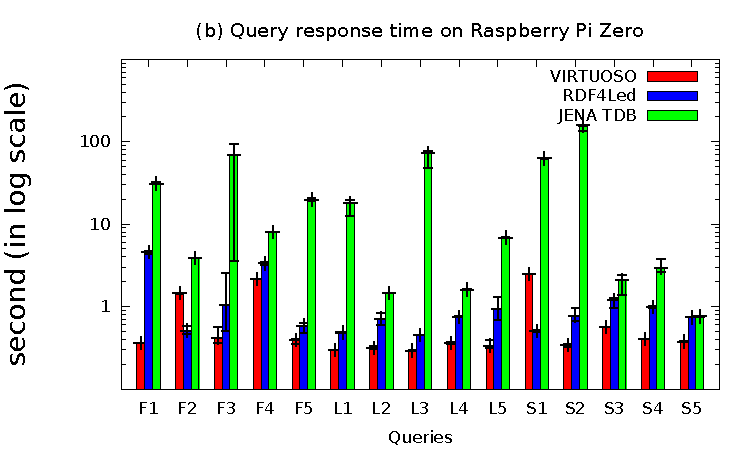
\includegraphics[width=0.3\textwidth]{c6/PI0_QUERY_WATDIV_100.pdf}
\label{fig:result_query}
\end{figure}

\begin{figure}[ht!]
\centering
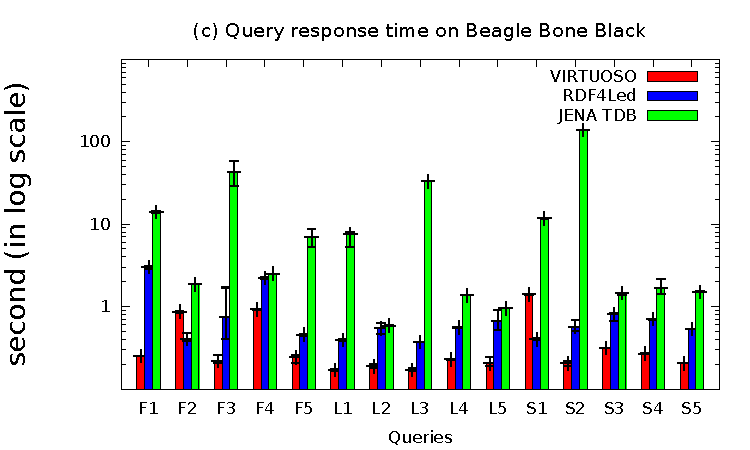
\includegraphics[width=0.3\textwidth]{c6/BBB_QUERY_WATDIV_100.pdf}
\label{fig:result_query}
\end{figure}

On all the devices, RDF4Led answered all the queries considerably faster than Jena TDB did. Both RDF4Led and JenaTDB follow the nested execution model to compute the multiple joins between RDF triples that match triple patterns. However, Jena TDB was implemented with iterator pattern, while RDF4Led followed the visitor pattern. In general, both algorithms execute lookup operations and index scan operations to extract the compatible triples from the dataset. The performance of these algorithms is mainly influenced by the performance of the lookup and index scan operations on the indexes. The better performance of RDF4Led against Jena TDB explains that our lightweight index structure helps RDF4Led outperform the B$+$ tree implemented in Jena TDB.  

\vspace{-1.5mm}
With the same dataset and on the same device, RDF4Led only answered the queries generated from templates F2 and S1 faster than Virtuoso does. These queries contain the graph patterns which have more than 6 triple patterns that form a star shape. In other cases, RDF4Led was slower than Virtuoso as it did not aggressively pre-allocate a fixed amount of memory (2-3 times more) for sophisticated optimisation algorithms. We see this as an option for improving query performance in our future work. However, in overall, at this current stage of the engine, RDF4Led can deliver reasonably good performance for up to 30 millions triples on this class of devices, e.g.  5 seconds at maximum and 1 second in average. This performance and scalability of RDF4Led can enable the devices of this kind to handle approximately 1 million sensor observations or 6 months worth data of 10 weather stations in an active RDF graph~\cite{Atemezing:2012}.   

\section{Summary}

%\chapter{Federated Edge}


Figure~\ref{fig:edge} illustrates the overview of a deployment of distributing data processing tasks to the edge of the IoT.
Similarly to a typical deployment of an IoT system, in the perceived layer, the low-end devices (e.g., sensors, actuators) can be deployed across several sites in different locations (e.g., houses or weather stations).
The devices in the same site can be connected to a gateway device that gives access to the produced data.
In IoT cloud-based systems~\cite{Petrolo:2014}, all the sensory data is pushed to cloud or a centralised node on which data integrating and data accessing take place.
In contrast of the deployments, we aim to push these tasks away from a centralised node by leveraging the advance computing resources of the gateway devices.
Therefore, we adopt mediator-based architecture~\cite{Garcia-molina:1995} in our model.
Gateway devices are attached a software component thus becoming mediators~\cite{Wiederhold:1992} for data integrating and accessing.
The mediator will allow physical data produced from the low-end devices to be wrapped into a common data model, and then to be stored on the gateways node.
Queries can be issued from a gateway, and can be federated to other connected gateways. 
The federation enables data to be accessed in the same manner as a centralised system. 

\begin{figure}[h!]
\centering
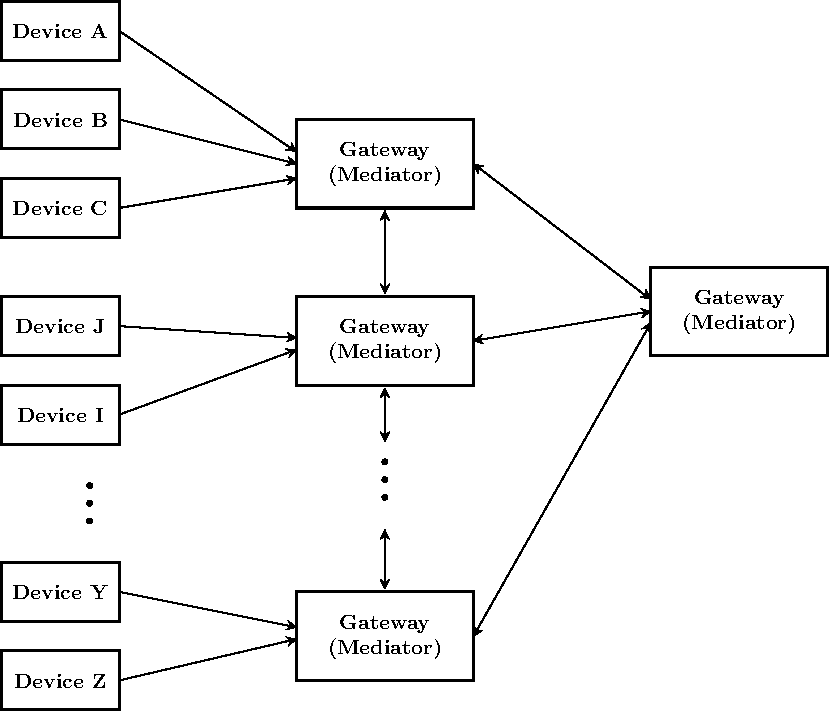
\includegraphics[width=0.35\textwidth]{c7/edge.pdf}
\caption{Overview of distributed architecture}
\label{fig:edge}
\end{figure}

In order to enable seamless integration across all the system, Linked Data technologies can be considered.
Since the high-end devices have enough computational resources, RDF engines can be brought to the gateway nodes to create such mediators.
Physical data from low-end devices can be wrapped into RDF data and can be locally stored using an RDF storage.
The federation mechanism of federated SPARQL queries can be also leveraged.
Simple data model of SPARQL federation such as RDF serialisation or SPARQL result can be used for information exchange between mediators.

\section{Gateway descriptor}

Semantic source selection: source can be select by it attributes.
why this is important. 

There are many approaches for source selection. Why do we need discovery???
each gateway is an endpoint - we can send ask query for each node for discovering.
We can use DHT to index source. From the subquery $\to$ select relevant source set.





In the IoT context, the sources are the \textit{"things"} which provide specific data, services.
Consumers cannot be asked to know the specific sources to navigate the federated queries.
Therefore, supporting automatic source discovery is one of major requirements for the mediators.
They should understand the meta-information of the connected things in the system, hence, 
query can be delivered to the mediators that things are connected.









A Thing in the system can be described using \textit{Thing Description (TD)}~\footnote{https://www.w3.org/TR/wot-thing-description/} framework. 
TD provides the syntax to describe the meta-information of thing (e.g., name of Thing, type of Thing), 
the interaction patterns (e.g., readable/writeable data on Thing, 
actions that can be triggered on Thing, events that are notified by Thing) and communication metadata.
TD can be represented using JSON-LD which is extremely lightweight and beneficial for constrained devices.
Listing~\ref{lst:TDexample} shows a sample TD of a temperature sensor named "MyTemperatureThing".
The sensor is serving a temperature reading as a Property.
The reading is accessible over CoAp protocol at the endpoint "coaps://mylamp.example.com:5683/" and is returned within a JSON-LD structure.


\begin{lstlisting}[language=sparql,
  				   captionpos=b,
                   label={lst:TDexample},
                   caption={SPARQL}]       
PREFIX sosa:<http://www.w3.org/ns/sosa/>                   
PREFIX ex:<http://example.org/featureOfInterest/>                   

SELECT ?tempValue ?windValue
{
 ?windObservation a sosa:Observation. 
 ?windObservation sosa:hasFeatureOfInterest ex:Wind.
 ?windObservation sosa:hasSimpleResult ?windValue.
 ?windObservation sosa:resultTime ?time.
 ?tempObservation a sosa:Observation.
 ?tempObservation sosa:hasFeatureOfInterest ex:Temperature.
 ?tempObservation sosa:hasSimpleResult ?tempValue.
 ?tempObservation sosa:resultTime ?time.
}
\end{lstlisting}



\begin{lstlisting}[language=sparql,
  				   captionpos=b,
                   label={lst:TDexample},
                   caption={Federated SPARQL}]
PREFIX sosa:<http://www.w3.org/ns/sosa/>                   
PREFIX ex:<http://example.org/featureOfInterest/>  

SELECT ?tempValue ?windValue {
SERVICE <ex:gatewayA> {
 ?windObservation a sosa:Observation. 
 ?windObservation sosa:hasFeatureOfInterest ex:Wind.
 ?windObservation sosa:hasSimpleResult ?windValue.
 ?windObservation sosa:resultTime ?time. }
SERVICE <ex:gatewayA> {
 ?tempObservation a sosa:Observation.
 ?tempObservation sosa:hasFeatureOfInterest ex:Temperature.
 ?tempObservation sosa:hasSimpleResult ?tempValue.
 ?tempObservation sosa:resultTime ?time.}
}
\end{lstlisting}

\begin{lstlisting}[language=sparql,
  				   captionpos=b,
                   label={lst:TDexample},
                   caption={Federated SPARQL}]
PREFIX sosa:<http://www.w3.org/ns/sosa/>                   
PREFIX ex:<http://example.org/featureOfInterest/>  

SELECT ?temp {
 ex:DeviceA ssn:hasSubSystem ?sensor
 ?sensor a sosa:Sensor.
 ?sensor sosa:madeObjervation ?observation.
 ?observation ex:hasValue ?temp.
}
\end{lstlisting}


\section{Source Selection}


\begin{lstlisting}[language=sparql,
  				   captionpos=b,
                   label={lst:TDexample},
                   caption={Federated SPARQL}]
PREFIX sosa:<http://www.w3.org/ns/sosa/>                   
PREFIX ex:<http://example.org/featureOfInterest/>  

SELECT ?tempValue {
 ?gateway ssn:Subsystem ?sensor
 ?sensor  a ssn:Sensor.
 ?sensor  a ex:Temperature.
 
 Service <?gateway>
 {
  ?tempObservation a sosa:Observation.
  ?tempObservation sosa:hasFeatureOfInterest ex:Temp.
  ?tempObservation sosa:hasSimpleResult ?tempValue.
  ?tempObservation sosa:resultTime ?time.
 }
}
\end{lstlisting}



The federated search consists of organizing service information in a set of information repositories and managing them to perform the service discovery tasks.
For example: If we want to query temperature data using sparql query.
The federator has to discover which mediator connects to temperature data.


\begin{lstlisting}[language=sparql,
  				   captionpos=b,
                   label={lst:TDexample},
                   caption={Simple TD example describing a mediator}]
SELECT ?temphref {
  ?device td:interaction ?property
  ?property a td:Property.
  ?property a iot:Temperature.
  ?property td:form ?form.
  ?form td:mediaType "application/jsonld"
  ?form td:href ?temphref.
}
\end{lstlisting}


Search criteria can be considered as the queries that trigger the discovery process which is expected to end up providing a ranked set of matching thing descriptions to the issuer. 
In case a query language, e.g., SPARQL is used for expressing semantic search criteria, all involved actors should at least know about its protocol, i.e., communications established between an issuer and a directory must implement the corresponding query language protocol. 
A high level of expressiveness of the query language used will likely broaden the possibilities
for discovery requests, e.g., features for filtering and aggregating.

Mediator:
Not exact match 
Reasoning $\to$ match
SPARQL Update $\to$ 


\begin{lstlisting}[language=sparql,
  				   captionpos=b,
                   label={lst:TDexample},
                   caption={Simple TD example describing a mediator}]
SELECT ?temphref {
  ?device td:interaction ?property
  ?property a td:Property.
  ?property a iot:Temperature.
  ?property td:form ?form.
  ?form td:mediaType "application/jsonld"
  ?form td:href ?temphref.
}
\end{lstlisting}











%\chapter{Conclusion}




Limitation of current rdf engine ~\note{Distribution of Semantic Reasoning on the Edge of Internet of Things}

\nop{
%RISC-style DBMS design
Chaudhuri and Weikum [2000] used the term RISC in their proposal for different
self-tuning RISC-style database system architecture. Their presented concepts are
inspired from RISC-based central processing unit (CPU) design, which advocates
the construction of a CPU using simpler and faster instructions instead of complex
and slow instructions [Patterson and Ditzel, 1980]. Use of complex instruction for
CPU design has its own benefits, which includes upward compatibility and better
marketing opportunities. We believe similar benefits as a factor that derived existing
DBMS components towards prevailing complexity. However, Patterson and
Ditzel [1980] discussed both approaches in the context of CPU design and presented
the benefits of RISC-based design, such as simple and fast instruction, a possibility
of careful pruning of an instruction set, and minimizing complexity to maximize performance.
We intend to achieve similar benefits in our RISC-style Cellular DBMS
architecture.

Chaudhuri and Weikum [2000] suggested the use of RISC-style data managers with
narrow functionality, specialized API, small footprint, and limited interaction. Their
aim is to reduce the number of tuning knobs for a DBMS to make it more predictable
in terms of performance and behavior making it easy to self-tune. They defended
their proposal with the notion of “gain/pain” ratio, which suggests to tolerate a
moderate degradation in “gain” with the introduction of overheads present in their
approach to reduce the “pain” related to tuning with more predictable performance.

}


%----------------------------------------------------------------------------------------
%	THESIS CONTENT - APPENDICES
%----------------------------------------------------------------------------------------

\addtocontents{toc}{} % Add a gap in the Contents, for aesthetics

\appendix % Cue to tell LaTeX that the following 'chapters' are Appendices

% Include the appendices of the thesis as separate files from the Appendices folder
% Uncomment the lines as you write the Appendices

%\chapter{Queries list}
\label{app:A}

\section{Linear joins queries}

%====================================================================================
\begin{lstlisting}[
captionpos=b, 
language=sparql,
basicstyle=\scriptsize\ttfamily,
title={L1 Search for ... }]
#Linear template L1
PREFIX sosa:<http://www.w3.org/ns/sosa/>

SELECT ?observation ?sensor ?station 
WHERE {
 ?observation sosa:hasFeatureOfInterest %featureOfInterest%.
 ?observation sosa:madeBySensor         ?sensor.
 ?sensor      sosa:isHostedBy           ?station.
}
\end{lstlisting}
%Checked
%====================================================================================
\begin{lstlisting}[
captionpos=b, 
language=sparql,
basicstyle=\scriptsize\ttfamily,
title={L2 - Search for ... }]
#Linear template L2
PREFIX sosa:<http://www.w3.org/ns/sosa/>
PREFIX iot:<http://insight.org/iot/data/noaa/>
PREFIX dul:<http://www.loa-cnr.it/ontologies/DUL.owl#>

SELECT ?observation 
WHERE {
  ?featureOfInterest  dul:hasLocation           ?location .
  ?observation        sosa:hasFeatureOfInterest ?featureOfInterest .
  ?observation        sosa:observedProperty     <iot:observableProperty/windSpeed/>.
}
\end{lstlisting}
%checked
%====================================================================================
\begin{lstlisting}[
captionpos=b, 
language=sparql,
basicstyle=\scriptsize\ttfamily,
title={L3 - Search for ... }]
#Linear template L3
PREFIX sosa:<http://www.w3.org/ns/sosa/>

SELECT ?observation ?sensor 
WHERE {
  ?observation sosa:madeBySensor ?sensor.
  ?observation sosa:hasFeatureOfInterest %featureOfInterest%.
}
%checked
\end{lstlisting}

%====================================================================================
\newpage
\begin{lstlisting}[
captionpos=b, 
language=sparql,
basicstyle=\scriptsize\ttfamily,
title={L4 - Search for ... }]
#Linear template L4
PREFIX sosa:<http://www.w3.org/ns/sosa/>

SELECT ?station ?sensor 
WHERE 
{
  ?station sosa:hosts ?sensor.
  ?station sosa:hasLocation %location%.
}
\end{lstlisting}
%checked
%====================================================================================
\begin{lstlisting}[
captionpos=b, 
language=sparql,
basicstyle=\scriptsize\ttfamily,
title={L5 - Search for ... }]
#Linear template L5
PREFIX sosa:<http://www.w3.org/ns/sosa/>

SELECT ?station ?sensor ?observation
WHERE 
{
  ?sensor        sosa:isHostedBy ?station.
  ?sensor        sosa:madeObservation ?observation.
  ?observation   sosa:hasFeatureOfInterest %featureOfInterest%.
}
\end{lstlisting}
%check
\section{Start joins queries}
%====================================================================================
\begin{lstlisting}[
captionpos=b, 
language=sparql,
basicstyle=\scriptsize\ttfamily,
title={S1 - Search for ... }]
PREFIX sosa:<http://www.w3.org/ns/sosa/>
PREFIX rdf:<http://www.w3.org/1999/02/22-rdf-syntax-ns#>

SELECT ?sensor ?observation ?featureOfInterest ?result ?time ?observableProperty
WHERE {
 ?sensor      sosa:madeObservation ?observation.
 ?observation sosa:hasFeatureOfInterest ?featureOfInterest.
 ?observation sosa:resultTime ?time.
 ?observation sosa:hasSimpleResult ?result.
 ?observation sosa:observedProperty ?observableProperty.
 ?observation rdf:type sosa:Observation.
}
\end{lstlisting}
%checked
%====================================================================================
\begin{lstlisting}[
captionpos=b, 
language=sparql,
basicstyle=\scriptsize\ttfamily,
title={S2 - Search for ... }]
PREFIX sosa:<http://www.w3.org/ns/sosa/>
PREFIX iot:<http://insight.org/dev/iot/noaa/>

SELECT ?observation ?sensor ?time 
WHERE {
 ?observation  sosa:madeBySensor         ?sensor.
 ?observation  sosa:hasFeatureOfInterest  %featureOfInterest%.
 ?observation  sosa:resultTime           ?time.
 ?observation  sosa:observedProperty      <iot:/observableProperty/windSpeed/>.
}
\end{lstlisting}
%checked
\newpage
%====================================================================================
\begin{lstlisting}[
captionpos=b, 
language=sparql,
basicstyle=\scriptsize\ttfamily,
title={S3 - Search for ... }]
PREFIX sosa:<http://www.w3.org/ns/sosa/>
PREFIX rdf:<http://www.w3.org/1999/02/22-rdf-syntax-ns#>

SELECT ?sensor ?station ?observation ?observableProperty 
WHERE {
 ?sensor rdf:type             %sensorType%.
 ?sensor sosa:isHostedBy      ?station.
 ?sensor sosa:madeObservation ?observation.
 ?sensor sosa:observes        ?observableProperty.
}
\end{lstlisting}
%checked
%====================================================================================
\begin{lstlisting}[
captionpos=b, 
language=sparql,
basicstyle=\scriptsize\ttfamily,
title={S4 - Find all   }]
PREFIX sosa:<http://www.w3.org/ns/sosa/>
PREFIX iot:<http://insight.org/dev/iot/noaa/>
PREFIX rdf:<http://www.w3.org/1999/02/22-rdf-syntax-ns#>

SELECT ?sensor ?observation ?station 
WHERE {
 ?sensor  rdf:type              %sensorType%.
 ?sensor  sosa:madeObservation  ?observation.
 ?station sosa:hosts            ?sensor.
 ?sensor  sosa:observes         <iot:observableProperty/windSpeed/>.
}
\end{lstlisting}
%checked
%====================================================================================
\begin{lstlisting}[
captionpos=b, 
language=sparql,
basicstyle=\scriptsize\ttfamily,
title={S5 - Find all   }]
PREFIX sosa:<http://www.w3.org/ns/sosa/>
PREFIX iot:<http://insight.org/dev/iot/noaa/>

SELECT ?observation ?time ?result 
WHERE {
 ?observation sosa:hasFeatureOfInterest %featureOfInterest%.
 ?observation sosa:resultTime	        ?time.
 ?observation sosa:hasSimpleResult      ?result.
 ?observation sosa:observedProperty     <iot:observableProperty/windSpeed/>.
}
\end{lstlisting}
%checked
\section{Snowflake joins queries}

%====================================================================================
\begin{lstlisting}[
captionpos=b, 
language=sparql,
basicstyle=\scriptsize\ttfamily,
title={F1 - Find all   }]
PREFIX sosa:<http://www.w3.org/ns/sosa/>
PREFIX rdf:<http://www.w3.org/1999/02/22-rdf-syntax-ns#>

SELECT ?sensor ?observation ?sensorType ?observableProperty ?result ?type
WHERE {
  ?sensor       rdf:type             ?sensorType.
  ?sensor       sosa:observes        ?observableProperty.
  ?observation  sosa:madeBySensor    ?sensor.
  ?observation  rdf:type             ?type.
  ?observation  sosa:resultTime      %time%.
  ?observation  sosa:hasSimpleResult ?result
}
%checked
\end{lstlisting}


\newpage
%====================================================================================
\begin{lstlisting}[
captionpos=b, 
language=sparql,
basicstyle=\scriptsize\ttfamily,
title={F2 - Find all   }]
PREFIX sosa:<http://www.w3.org/ns/sosa/>
PREFIX rdf:<http://www.w3.org/1999/02/22-rdf-syntax-ns#>

SELECT ?observation     ?sensor     ?featureOfInterest ?time ?result 
       ?observationType ?sensorType 
WHERE {
   ?observation sosa:hasFeatureOfInterest ?featureOfInterest.
   ?observation sosa:resultTime           ?time.
   ?observation sosa:hasSimpleResult      ?result.
   ?observation sosa:observedProperty     %observableProperty%.
   ?observation rdf:type                  ?observationType.
   ?observation sosa:madeBySensor         ?sensor.
   ?sensor      sosa:isHostedBy           ?station.
   ?sensor      rdf:type                  ?sensorType.
}
\end{lstlisting}
%checked
%====================================================================================
\begin{lstlisting}[
captionpos=b, 
language=sparql,
basicstyle=\scriptsize\ttfamily,
title={F3 - Find all   }]
PREFIX sosa:<http://www.w3.org/ns/sosa/>
PREFIX iot:<http://insight.org/dev/iot/noaa/>
PREFIX rdf:<http://www.w3.org/1999/02/22-rdf-syntax-ns#>

SELECT ?sensor ?station ?type ?location ?point ?name ?lat ?lon.
WHERE { 
?observation       sosa:hasSimpleResult       ?result.
?featureOfInterest sosa:isFeatureOfInterestOf ?observation.
?observation       sosa:madeBySensor          ?sensor.
?sensor            sosa:observes              ?observableProperty.
?sensor            sosa:isHostedBy            ?platform.
?sensor            rdf:type                   %sensorType%.
}
\end{lstlisting}
%checked
%====================================================================================
\begin{lstlisting}[
captionpos=b, 
language=sparql,
basicstyle=\scriptsize\ttfamily,
title={F4 - Find all   }]
PREFIX ssn:<http://www.w3.org/ns/ssn/>
PREFIX sosa:<http://www.w3.org/ns/sosa/>
PREFIX wgs84:<http://www.w3.org/2003/01/geo/wgs84_pos#>
PREFIX dul:<http://www.loa-cnr.it/ontologies/DUL.owl#>
PREFIX geo:<http://www.geonames.org/ontology#>

SELECT ?featureOfInterest ?result ?observation
WHERE { 
  ?featureOfInterest ssn:hasProperty <http://insight.org/iot/data/noaa/observableProperty/windSpeed/>.
  ?featureOfInterest dul:hasLocation ?location.
  ?location wgs84:point ?point.
  ?point    wgs84:lat %lat%.
  ?point    wgs84:lon %lon%.
  ?featureOfIterest sosa:isFeatureOfInterestOf ?observation.
  ?observation sosa:resultTime %time%.
  ?observation sosa:hasSimpleResult ?result.
}
\end{lstlisting}
%checked
\section{Complex}

%====================================================================================
\begin{lstlisting}[captionpos=b, 
language=sparql,
title=Query 1. List all the temperature values from a given location and order by time,
basicstyle=\ttfamily,frame=single]
PREFIX sosa:<http://www.w3.org/ns/sosa/>
PREFIX wgs84:<http://www.w3.org/2003/01/geo/wgs84_pos#>
PREFIX dul:<http://www.loa-cnr.it/ontologies/DUL.owl#>
PREFIX geo:<http://www.geonames.org/ontology#>
PREFIX rdf:<http://www.w3.org/1999/02/22-rdf-syntax-ns#>

SELECT ?result ?time
WHERE
{
    ?station       dul:hasLocation       ?location.
    ?location      wgs84:Point           ?point.
    ?point         wgs84:lat             %lat%.
    ?point         wgs84:lon             %lon%.
    ?station       sosa:hosts            ?sensor.
    ?sensor        rdf:type              <http://insight.org/iot/data/noaa/class/temperatureSensor/>.
    ?sensor        sosa:madeObservation  ?observation.
    ?observation   sosa:observedProperty <http://insight.org/iot/data/noaa/observableProperty/temperature/>.
    ?observation   sosa:resultTime       ?time.
    ?observation   sosa:hasSimpleResult  ?result.
}
ORDER BY (?time)
\end{lstlisting}
%checked
%====================================================================================

{
\begin{lstlisting}[captionpos=b, 
title=Query 2. Return the average temperature in each month of a given station,
language=sparql,
basicstyle=\ttfamily,frame=single]
PREFIX rdf:<http://www.w3.org/1999/02/22-rdf-syntax-ns#>
PREFIX sosa:<http://www.w3.org/ns/sosa/>

SELECT ?month (avg(?re) as ?TempAVG)

WHERE
{
    %station%      sosa:hosts            ?sensor.
    ?sensor        rdf:type              <http://insight.org/iot/data/noaa/class/temperatureSensor/>.
    ?sensor        sosa:madeObservation  ?observation.
    ?observation   sosa:observedProperty <http://insight.org/iot/data/noaa/observableProperty/temperature/>.
    ?observation   sosa:resultTime       ?time.
    ?observation   sosa:hasSimpleResult  ?result.
}
GROUP BY (month(?time) as ?month)
\end{lstlisting}
}
%checked
%====================================================================================
{
\begin{lstlisting}[captionpos=b, 
language=sparql,
title=Query 3. Search for the date that has highest temperature in a given station
basicstyle=\ttfamily,
frame=single]
PREFIX rdf:<http://www.w3.org/1999/02/22-rdf-syntax-ns#>
PREFIX sosa:<http://www.w3.org/ns/sosa/>

SELECT ?day ?month (max(?TempValue) as ?TempMax)

WHERE
{
 %station%      sosa:hosts             ?sensor.
 ?sensor        rdf:type               <http://insight.org/iot/data/noaa/class/temperatureSensor/>.
 ?sensor        sosa:madeObsevation    ?observation.
 ?observation   sosa:observedProperty  <http://insight.org/iot/data/noaa/observableProperty/temperature/>.
 ?observation   sosa:resultTime        ?time.
 ?observation   sosa:hasSimpleResult   ?result.
}
GROUP BY (day(?time) as ?day) (month(?time) as ?month)
\end{lstlisting}
}
%checked
%====================================================================================
\newpage
\begin{lstlisting}[captionpos=b, 
title=Query 4. Search for the hottest place,
language=sparql,
basicstyle=\ttfamily,
frame=single]
PREFIX sosa:<http://www.w3.org/ns/sosa/>
PREFIX iot:<http://insight.org/dev/iot/noaa/>
PREFIX wgs84:<http://www.w3.org/2003/01/geo/wgs84_pos#>
PREFIX dul:<http://www.loa-cnr.it/ontologies/DUL.owl#>
PREFIX geo:<http://www.geonames.org/ontology#>

SELECT ?maxValue ?lat ?long ?name.

WHERE
{
  {
 	SELECT ?observation (MAX(?result) as ?maxValue)
    {
      ?observation   sosa:observedProperty  <http://insight.org/iot/data/noaa/observableProperty/temperature/>.
      ?observation   sosa:resultTime      ?time.
      ?observation   sosa:hasSimpleResult ?result.
    }
  }
  ?observation sosa:madeBySensor ?sensor.
  ?sensor      sosa:isHostedBy   ?station.
  ?station     dul:hasLocation   ?location.
  ?location    wgs84:Ooint       ?point.
  ?point       geo:name          ?name.
  ?point       wgs84:lat         ?lat.
  ?point       wgs84:lon         ?lon.
}
\end{lstlisting}
%checked
%====================================================================================
\section{Federated Query}

\addtocontents{toc}{} % Add a gap in the Contents, for aesthetics

\backmatter

%----------------------------------------------------------------------------------------
%	BIBLIOGRAPHY
%----------------------------------------------------------------------------------------

\label{Bibliography}

\lhead{\emph{Bibliography}} % Change the page header to say "Bibliography"

\bibliography{Bibliography} % The references (bibliography) information are stored in the file 

\end{document}  